\documentclass[12pt,a4paper]{article}

\usepackage[margin=1in]{geometry}
\usepackage[T1]{fontenc}
\usepackage[utf8]{inputenc}
\usepackage{lmodern}
\usepackage{textcomp}
\usepackage{parskip}
\usepackage{graphicx}
\usepackage{setspace}
\usepackage{float}
\usepackage[section]{placeins}
\usepackage{booktabs}
\usepackage{array}
\usepackage{longtable}
\usepackage{caption}
\usepackage{subcaption}
\usepackage{pgfgantt}
\usepackage{enumitem}
\usepackage{amsmath,amssymb}
\usepackage{siunitx}
\usepackage{tabularx}
\usepackage{qrcode}
\usepackage[hidelinks]{hyperref}
\usetikzlibrary{positioning, arrows.meta, fit, backgrounds, calc}

\newcolumntype{L}[1]{>{\raggedright\arraybackslash}p{#1}}
\renewcommand{\arraystretch}{1.35}
\captionsetup{font=small,labelfont=bf,skip=6pt}
\setlist[itemize]{topsep=2pt,itemsep=2pt,parsep=0pt,leftmargin=1.5em}
\sisetup{detect-weight=true, detect-family=true}

% Gantt chart styles (Section~\ref{sec:gantt})
\definecolor{ganttpast}{HTML}{8FC98F}
\definecolor{ganttnow}{HTML}{F5A25D}
\definecolor{ganttnext}{HTML}{DADADA}
\ganttset{
	gantt style/.style={
		time slot format=isodate, x unit=0.045cm, y unit title=0.45cm,
		y unit chart=0.335cm, hgrid={*1{black!8}}, vgrid={*6{draw=none}, *1{black!12}},
		title/.append style={draw=black!40, fill=black!6},
		title label font=\scriptsize, bar label font=\scriptsize,
		milestone label font=\scriptsize, group label font=\scriptsize\bfseries,
		bar height=0.55, bar/.append style={draw=black!50},
		group/.append style={fill=black!65, draw=none}, group height=0.25,
		group right shift=0, group left shift=0, group top shift=0.4,
		milestone left shift=-2, milestone right shift=2,
		milestone/.append style={draw=black!60},
		vrule/.append style={draw=red!70!black, dashed, thick},
		vrule label font=\scriptsize\bfseries\color{red!70!black},
	},
	gpast/.style={bar/.append style={fill=ganttpast}, milestone/.append style={fill=ganttpast}},
	gnow/.style={bar/.append style={fill=ganttnow}, milestone/.append style={fill=ganttnow},
		bar label font=\scriptsize\bfseries, milestone label font=\scriptsize\bfseries},
	gnext/.style={bar/.append style={fill=ganttnext}, milestone/.append style={fill=ganttnext}},
}
% Colours for the teleoperation / embedded diagrams (Section~\ref{sec:teleop-architecture})
\definecolor{pcblue}{RGB}{225,236,250}
\definecolor{espgreen}{RGB}{226,243,228}
\definecolor{stmorange}{RGB}{253,236,220}
\definecolor{hwgray}{RGB}{238,238,238}
\definecolor{linkred}{RGB}{170,40,40}

\DeclareRobustCommand{\ganttkey}[1]{\tikz[baseline=-0.6ex]\fill[#1, draw=black!50] (0,-0.12) rectangle (0.35,0.12);}

% Placeholder-safe figure: grey box until the image exists.
\providecommand{\figOrBox}[2]{%
  \IfFileExists{#2}{\includegraphics[width=#1]{#2}}%
  {\fbox{\parbox[c][0.3\textheight][c]{\dimexpr#1-2\fboxsep-2\fboxrule\relax}{\centering\small TODO: \detokenize{#2}}}}}

\begin{document}

%---------------------------------------------------------------- title page --
% Cover from Proposal.tex (ISE format), retitled for the progress report.
\begin{titlepage}
\centering
\setstretch{1.0}
\vspace*{0cm}

{\Large\bfseries Capstone Design Project I\par}
\vspace{0.3cm}
{\large Progress Report 3 (Short Version)\par}

\vspace{0.6cm}

\includegraphics[width=3.2cm]{../image/chula_eng_logo.png}\par
\vspace{0.6cm}

{\Large\bfseries A Modular Self-Reconfigurable Robot (MSRR)\\[0.35em]
for Search and Space Exploration\par}

\vspace{0.7cm}
{Submitted to the\par}
{Project Committee appointed by the\par}
{International School of Engineering (ISE)\par}
{Faculty of Engineering, Chulalongkorn University\par}

\vspace{0.6cm}
{\bfseries Project Advisors\par}
\vspace{0.35cm}
{Asst.\ Prof.\ Paulo Fernando Rocha Garcia, Ph.D.\par}
{Asst.\ Prof.\ Surat Kwanmuang, Ph.D.\par}

\vspace{0.6cm}
{\bfseries Submitted By\par}
\vspace{0.45cm}
\begin{tabular}{@{}l@{\hspace{2em}}l@{}}
Kittivut Pipattanachaiyapong  & 6638019121 \\
Krin Kaweewongsonthorn        & 6638027121 \\
Pakapol Kijsupanont           & 6638172421 \\
Phattharamon Sukvivatn        & 6638178221 \\
\end{tabular}

\vfill
{\footnotesize 1/2026: 2147498 Capstone Design Project I\par}
{\footnotesize Robotics and Artificial Intelligence Engineering (International
Program)\par}
{\footnotesize International School of Engineering (ISE), Faculty of Engineering,\par}
{\footnotesize Chulalongkorn University\par}
\end{titlepage}

% ================================================================
\section{Project Timeline}
% ================================================================

\begin{itemize}
	\item \textbf{Completed:} Project concept, objectives, literature review, and
	      phased system architecture established.
	\item \textbf{In progress:} Phase A --- single-module locomotion, sensing,
	      communication, and simulation baseline.
	\item \textbf{Next:} Phase B --- EP-Face docking, task-oriented
	      reconfiguration, and simple assembled locomotion.
\end{itemize}

% ================================================================
\section{Project Phases}
% ================================================================

\subsection{Phase A}
External perception and computation. Develop the mechanically homogeneous
module, differential-drive locomotion, joint control, odometry, and
module-to-commander communication. Validate the module and physics twin before
physical docking is introduced.

\subsection{Phase B}
Docking and task-oriented reconfiguration. Add the electropermanent EP-Face
connectors, infrared alignment, and connector-state feedback. Extend the
reconfiguration pipeline with task assignment, parallel assembly sequencing,
and selection from a library of feasible configurations.

\subsection{Phase C}
Onboard perception with external computation. Mount a monocular RGB camera and
an $8\times8$ multi-zone ToF sensor on the leader module. Estimate obstacle
geometry and traversability locally, while transmitting sensor data to an
external computer for processing.

\subsection{Phase D}
Fully onboard perception and computation. Move the perception and
configuration-selection pipeline onto a coordinator module using an embedded
compute board. Close the perceive--select--reconfigure--traverse loop on
hardware without external localisation or computation.

\clearpage
% ================================================================
\section{Gantt Chart}
\label{sec:gantt}
% ================================================================

Task schedule from the team Notion timeline (as of 20~Nov~2026), grouped by phase.

\begin{figure}[H]
\centering\scriptsize
\begin{ganttchart}[gantt style]{2026-08-17}{2027-03-21}
\gantttitlecalendar{year, month=shortname} \\
\ganttgroup{Phase A --- Locomotion, sensing and communication}{2026-08-28}{2027-01-04} \\
\ganttbar[gpast]{(Phase\_A\_1) Electronics Planning/ Trade Study}{2026-08-28}{2026-09-30} \\
\ganttmilestone[gpast]{MILESTONE - Proposal submission}{2026-08-28} \\
\ganttbar[gpast]{Module design Mechanic Draft 1 (CAD)}{2026-08-28}{2026-09-17} \\
\ganttbar[gpast]{Module design Mechanic Draft 1 (FAB) Draft\_1}{2026-09-18}{2026-10-12} \\
\ganttbar[gpast]{(sim) export URDF to gazebo, controller and locomotion}{2026-09-25}{2026-10-08} \\
\ganttmilestone[gpast]{MILESTONE - First progress report}{2026-09-25} \\
\ganttbar[gnow]{(Phase\_A\_1) Part Ordering/Shipping}{2026-10-01}{2026-10-15} \\
\ganttbar[gpast]{Control board and firmware}{2026-10-01}{2026-10-10} \\
\ganttbar[gpast]{Power, Main Board PCB Designing}{2026-10-01}{2026-10-15} \\
\ganttbar[gpast]{Gear and Shaft Print Testing and Redesign}{2026-10-05}{2026-10-25} \\
\ganttbar[gpast]{(sim) Implement Reconfiguration planning}{2026-10-09}{2026-11-03} \\
\ganttbar[gnow]{(sim) Navigation and avoidance with known coordinate}{2026-10-09}{2026-10-21} \\
\ganttbar[gpast]{Basic Locomotion Testing}{2026-10-13}{2026-10-20} \\
\ganttbar[gnow]{(Phase\_A\_1) Testing}{2026-10-16}{2026-11-21} \\
\ganttbar[gnow]{(real) Localization and navigation from camera}{2026-10-23}{2026-11-03} \\
\ganttmilestone[gpast]{MILESTONE - Second progress report}{2026-10-23} \\
\ganttbar[gnow]{(real) Implement Reconfiguration planning}{2026-11-04}{2026-11-18} \\
\ganttbar[gnow]{low level control + Sensing IMU Encoder (Dev board)}{2026-11-08}{2026-11-21} \\
\ganttbar[gnext]{Connector FAB (EP-Face) (1)}{2026-11-15}{2026-11-30} \\
\ganttbar[gnow]{Power, Main Board PCB FAB + Part Ordering}{2026-11-15}{2026-12-04} \\
\ganttbar[gnow]{UWB \& Radio link wifi testing (Dev board)}{2026-11-25}{2026-12-08} \\
\ganttbar[gnext]{Power, Main Board Testing}{2026-12-05}{2026-12-18} \\
\ganttbar[gnow]{Radio link and protocol}{2026-12-08}{2026-12-21} \\
\ganttbar[gnext]{Connector design (EP-Face)}{2026-12-19}{2027-01-04} \\
\ganttgroup{Phase B --- Docking and task-oriented reconfiguration}{2026-10-01}{2027-03-14} \\
\ganttbar[gpast]{EP Research and Face Design}{2026-10-01}{2026-10-25} \\
\ganttbar[gpast]{EP Face Part Ordering}{2026-10-26}{2026-11-10} \\
\ganttbar[gnow]{(sim) urdf add contact face}{2026-11-05}{2026-11-18} \\
\ganttbar[gnow]{EP Face 1st Test}{2026-11-11}{2027-01-16} \\
\ganttbar[gnow]{Contract face testing}{2026-11-13}{2026-11-26} \\
\ganttmilestone[gnow]{MILESTONE - Draft final report}{2026-11-18} \\
\ganttbar[gnow]{(sim) precision docking with self alignment}{2026-11-20}{2026-12-03} \\
\ganttbar[gnext]{MILESTONE - Final presentation}{2026-11-22}{2026-12-03} \\
\ganttbar[gnext]{Locomotion with contact face testing}{2026-11-27}{2026-12-10} \\
\ganttbar[gnow]{(real) Reconfiguration planning with precision docking}{2026-12-04}{2026-12-17} \\
\ganttbar[gnext]{IR Face Design}{2026-12-04}{2026-12-18} \\
\ganttmilestone[gnext]{MILESTONE - Final report (Project I)}{2026-12-10} \\
\ganttbar[gnext]{Assembled gaits, PPO training}{2026-12-11}{2027-01-03} \\
\ganttbar[gnext]{Configuration library}{2026-12-11}{2026-12-27} \\
\ganttbar[gnext]{EP-Face build and characterisation}{2026-12-11}{2027-01-03} \\
\ganttbar[gnext]{IR alignment and docking}{2026-12-11}{2026-12-27} \\
\ganttbar[gnext]{IR Face Part Ordering}{2027-01-01}{2027-01-11} \\
\ganttbar[gnext]{IR 1st test}{2027-01-12}{2027-01-25} \\
\ganttbar[gnext]{In-Wheel (EP and IR) Board Designing}{2027-02-01}{2027-02-14} \\
\ganttbar[gnext]{In-Wheel (EP and IR) Board FAB + Part Ordering}{2027-02-15}{2027-02-28} \\
\ganttbar[gnext]{In-Wheel (EP and IR) Board Testing}{2027-03-01}{2027-03-14}
\ganttvrule{Today (20 Nov)}{2026-11-20}
\end{ganttchart}
\caption{Project I schedule (Phases A--B). \ganttkey{ganttpast}~Completed \quad \ganttkey{ganttnow}~In progress \quad \ganttkey{ganttnext}~Upcoming; dashed line marks the report date.}
\label{fig:gantt-ab}
\end{figure}

\begin{figure}[H]
\centering\scriptsize
\begin{ganttchart}[gantt style]{2026-12-07}{2027-04-30}
\gantttitlecalendar{year, month=shortname} \\
\ganttgroup{Phase C --- Onboard perception, external computation}{2026-12-13}{2027-03-05} \\
\ganttbar[gnext]{(sim) Environment classification}{2026-12-13}{2027-01-18} \\
\ganttbar[gnext]{(sim) onboard perception obstacle avoidance and navigation}{2026-12-13}{2026-12-31} \\
\ganttbar[gnext]{Onboard perception testing}{2026-12-24}{2027-01-06} \\
\ganttbar[gnext]{(Real) Onboard Perception nav and configuration planning}{2027-01-01}{2027-01-18} \\
\ganttbar[gnext]{Locomotion, Planning with internal Perception (IR and UWB)}{2027-01-03}{2027-01-31} \\
\ganttbar[gnext]{Camera and ToF integration}{2027-01-04}{2027-02-12} \\
\ganttbar[gnext]{Inductive Encoder Designing}{2027-01-05}{2027-01-20} \\
\ganttbar[gnext]{Policy training on held-out params}{2027-01-11}{2027-02-26} \\
\ganttbar[gnext]{Obstacle state to configuration}{2027-01-18}{2027-03-05} \\
\ganttbar[gnext]{(sim) Configuration lookup table}{2027-01-19}{2027-02-01} \\
\ganttbar[gnext]{Inductive Encoder FAB + Part Ordering}{2027-01-21}{2027-02-10} \\
\ganttbar[gnext]{Terrain and traversability pipeline}{2027-01-25}{2027-03-05} \\
\ganttbar[gnext]{(Real) environment adaptation}{2027-02-02}{2027-02-28} \\
\ganttbar[gnext]{Inductive Encoder Testing}{2027-02-11}{2027-02-28} \\
\ganttbar[gnext]{MILESTONE - Phase C evaluation}{2027-03-01}{2027-03-05} \\
\ganttgroup{Phase D --- Fully onboard perception and computation}{2027-01-21}{2027-04-30} \\
\ganttbar[gnext]{PCB for CM5 Designing}{2027-01-21}{2027-02-04} \\
\ganttbar[gnext]{PCB for CM5 Designing FAB + Part Ordering}{2027-02-05}{2027-02-18} \\
\ganttbar[gnext]{Compute module bring-up}{2027-02-15}{2027-03-19} \\
\ganttbar[gnext]{CM5 with RGBD and TOF Testing}{2027-02-19}{2027-03-04} \\
\ganttbar[gnext]{Onboard Odometry with no camera testing}{2027-02-22}{2027-03-11} \\
\ganttbar[gnext]{Onboard odometry, drop VICON}{2027-02-22}{2027-04-02} \\
\ganttbar[gnext]{(sim) local interaction to reorganize (concept)}{2027-03-01}{2027-04-09} \\
\ganttbar[gnext]{Full testing internal computation}{2027-03-01}{2027-04-02} \\
\ganttbar[gnext]{Internal Computation}{2027-03-01}{2027-03-14} \\
\ganttbar[gnext]{Quantised inference on module}{2027-03-08}{2027-04-09} \\
\ganttbar[gnext]{MILESTONE - Loop closed on hardware}{2027-04-05}{2027-04-09} \\
\ganttbar[gnext]{MILESTONE - Final evaluation (Project II)}{2027-04-26}{2027-04-30}
\end{ganttchart}
\caption{Project II schedule (Phases C--D). All tasks upcoming (\ganttkey{ganttnext}).}
\label{fig:gantt-cd}
\end{figure}

% ================================================================
\section{Module CAD Design}
\label{sec:module-cad-design}
% ================================================================

The design is based on SMORES-EP \cite{tosun2016} (originally \SI{80}{mm}), scaled to a $100 \times 100 \times 100$\,mm envelope for additional packaging space. The CAD design, gear train derivation and face geometry are unchanged since Progress Report~2 and are only summarised here.

% ----------------------------------------------------------------
\subsection{Assembled Prototype}
\label{sec:assembled-prototype}

Figure~\ref{fig:real-views} shows the physically
assembled module, with printed wheels, pan and tilt faces, spur and crown gears,
and N20 motors mounted in the frame.

\begin{figure}[!htbp]
	\centering
	\begin{subfigure}[b]{0.31\textwidth}
		\centering
		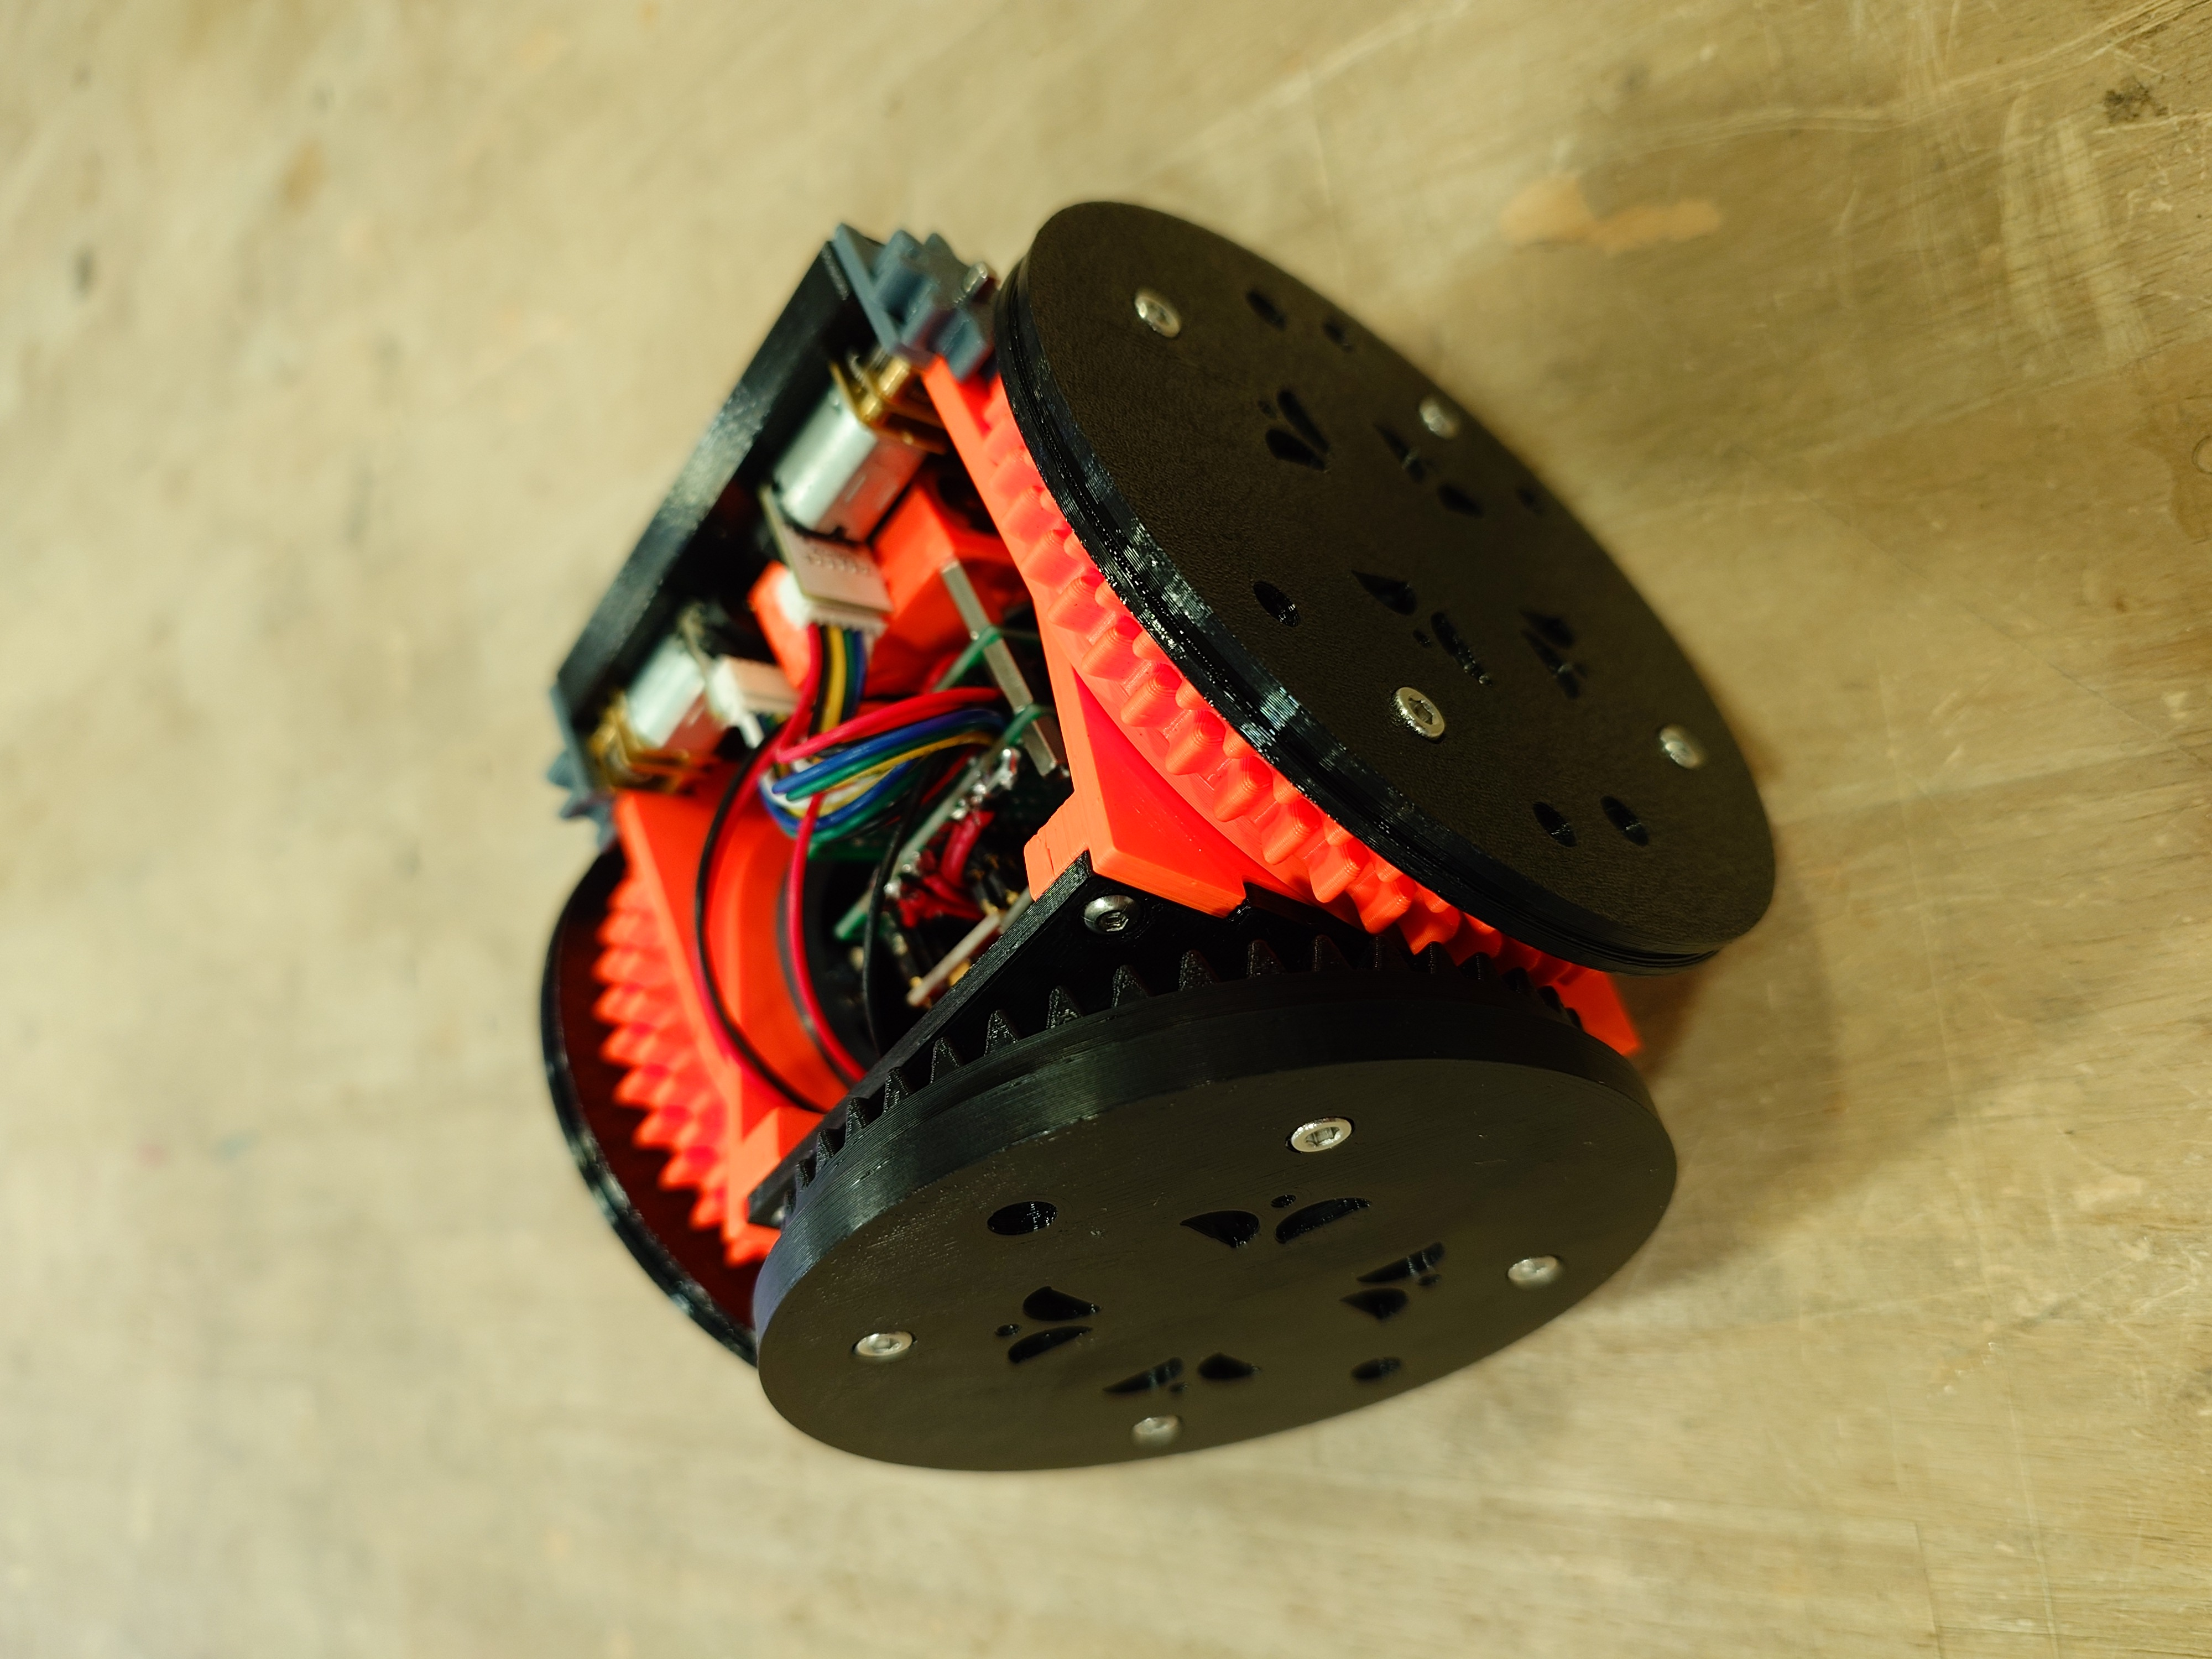
\includegraphics[width=\linewidth,height=3.4cm,keepaspectratio]{../image/assembled_iso_view.jpg}
		\caption{Oblique view of the pan face and crown gear.}
		\label{fig:real-iso}
	\end{subfigure}
	\hfill
	\begin{subfigure}[b]{0.31\textwidth}
		\centering
		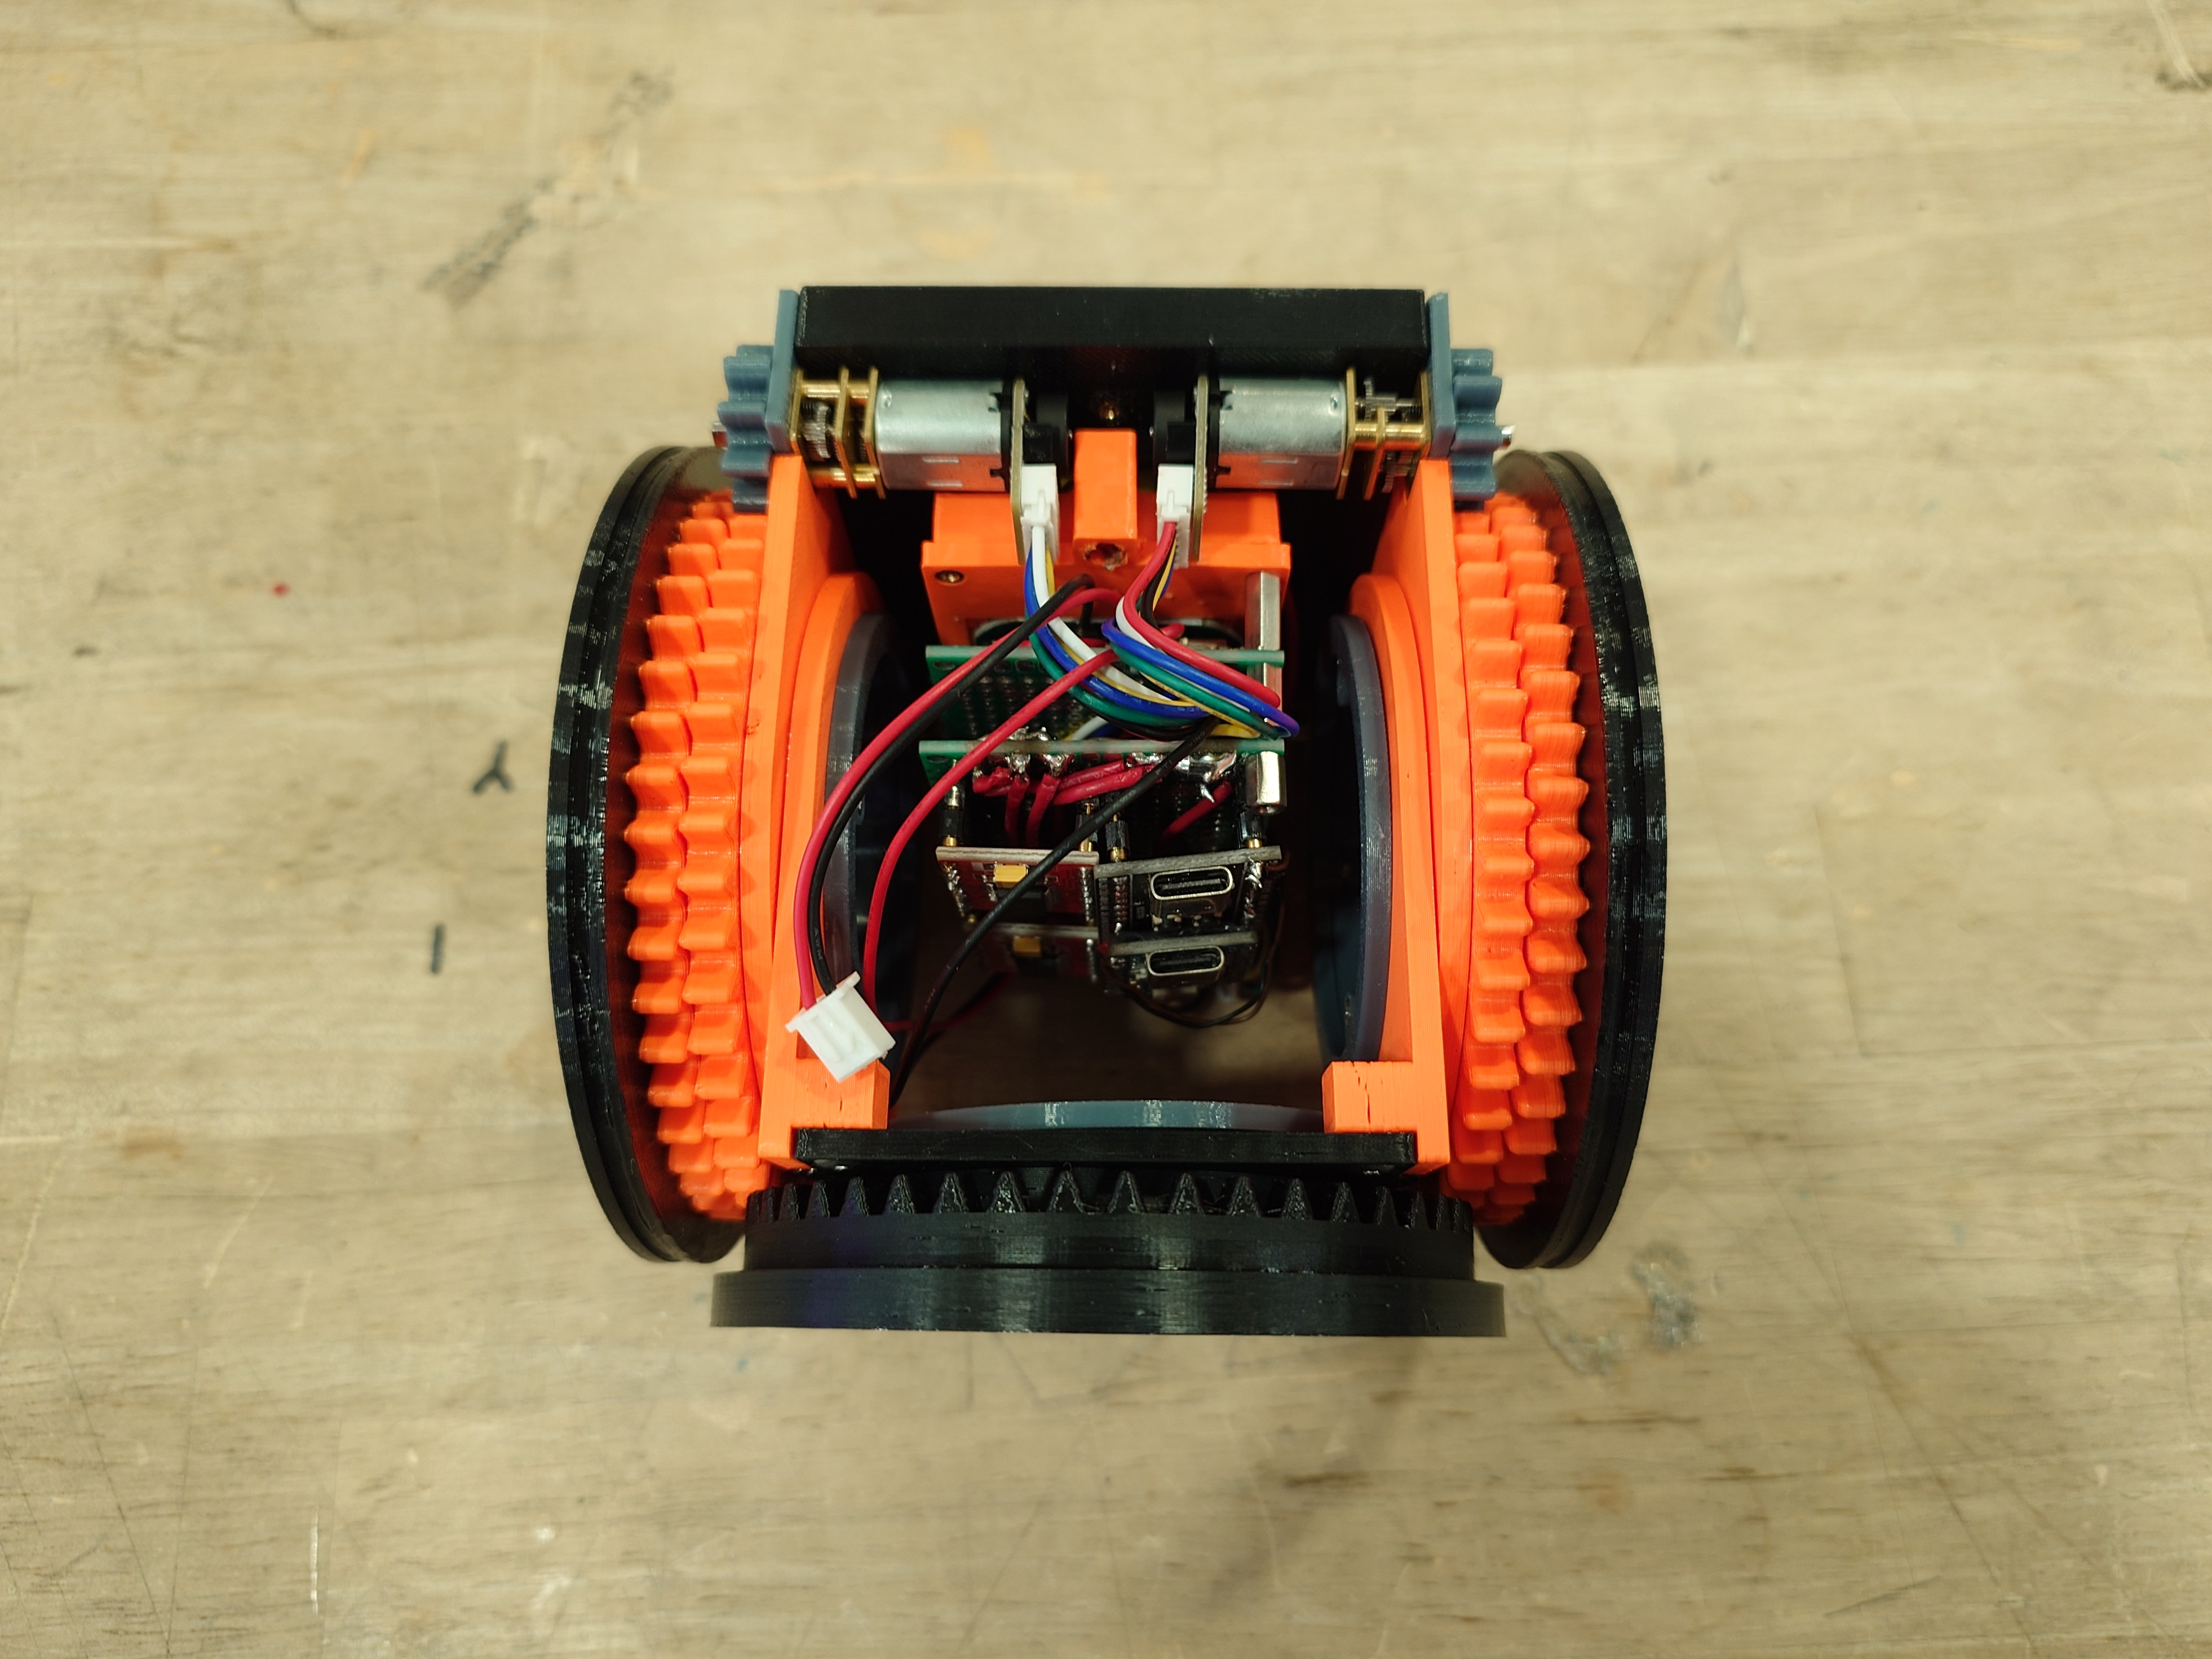
\includegraphics[width=\linewidth,height=3.4cm,keepaspectratio]{../image/assembled_top_view.jpg}
		\caption{Top view of wheels, spur gears, and frame.}
		\label{fig:real-top}
	\end{subfigure}
	\hfill
	\begin{subfigure}[b]{0.31\textwidth}
		\centering
		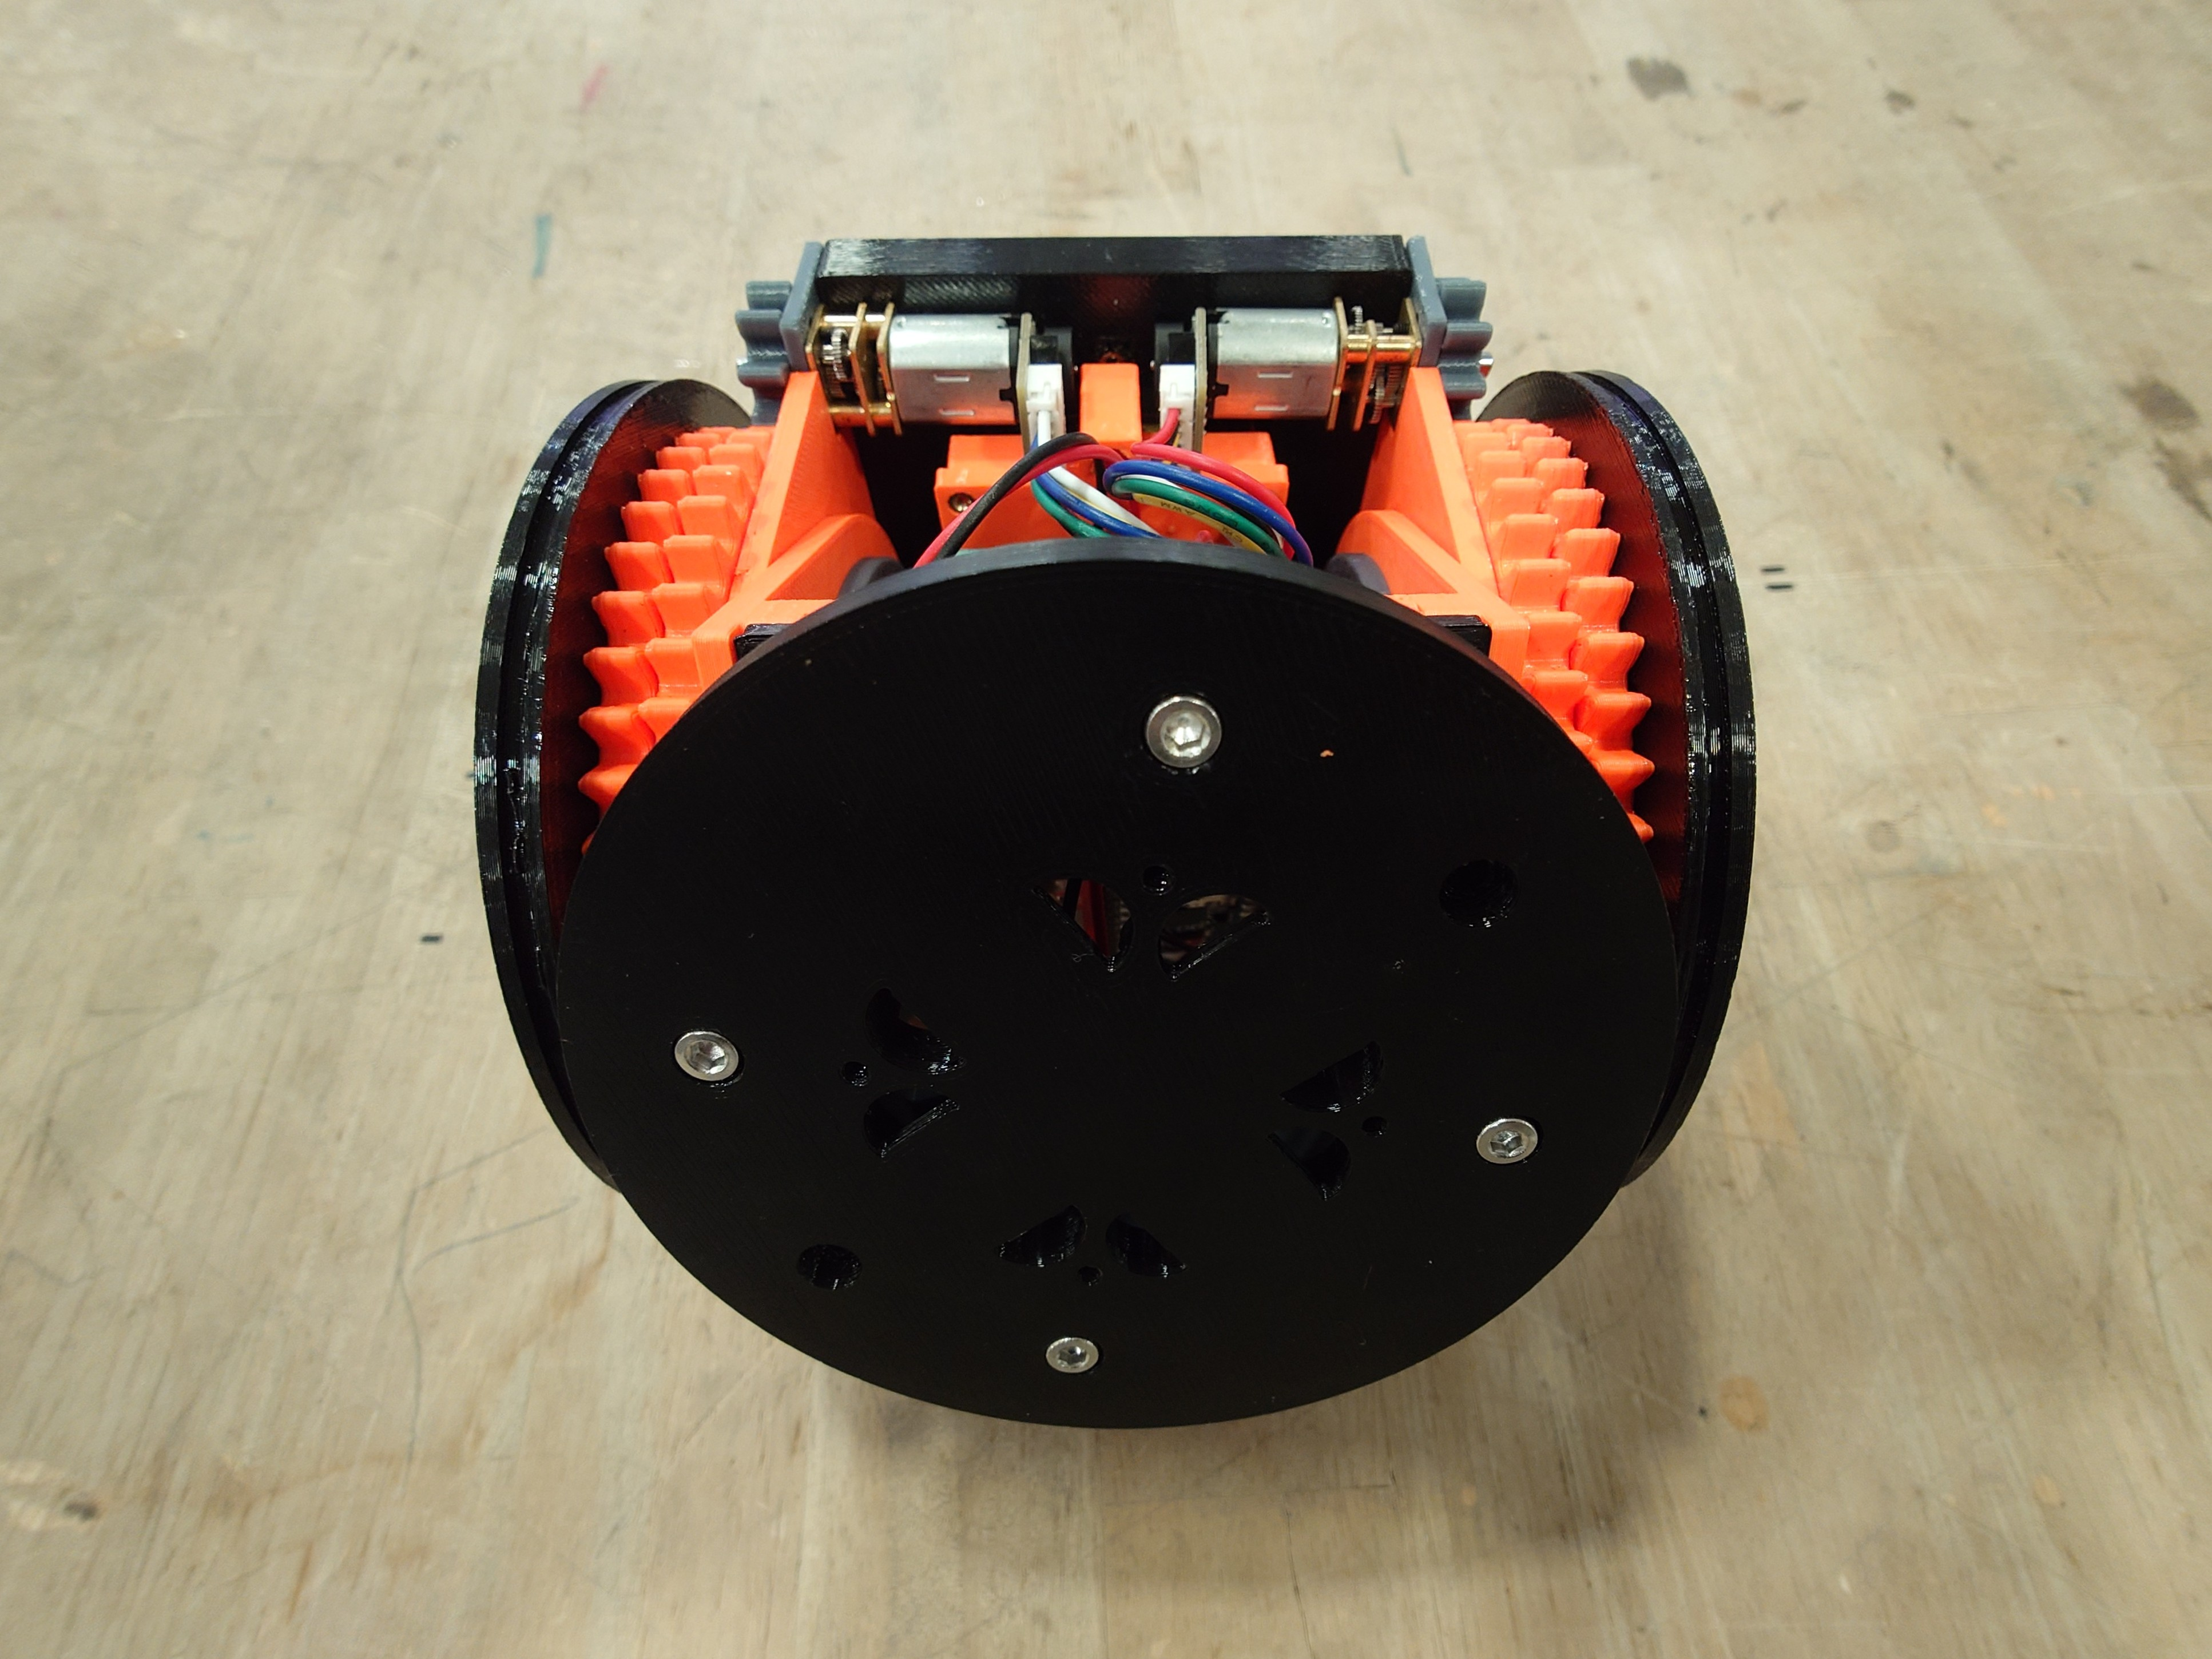
\includegraphics[width=\linewidth,height=3.4cm,keepaspectratio]{../image/assembled_tilt_face.jpg}
		\caption{Tilt face with EP-magnet openings.}
		\label{fig:real-tilt}
	\end{subfigure}
	\par\vspace{6pt}
	\begin{subfigure}[b]{0.31\textwidth}
		\centering
		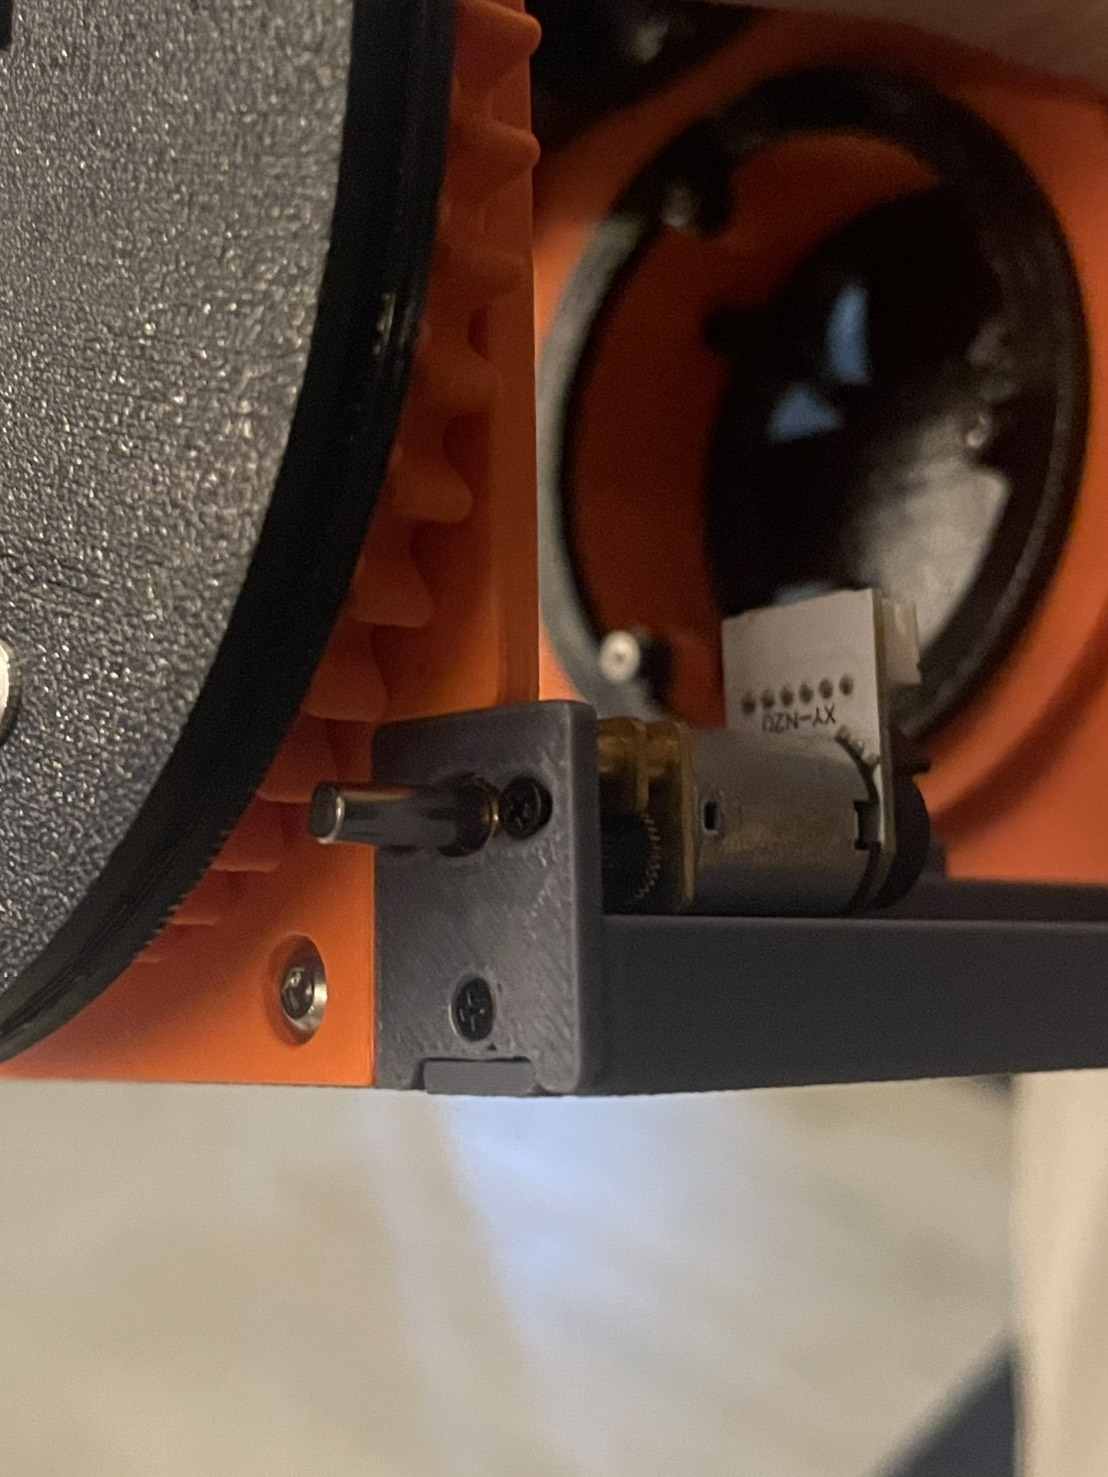
\includegraphics[width=\linewidth,height=3.4cm,keepaspectratio]{../image/assembled_motor_mount.jpg}
		\caption{N20 gearmotor in its printed mount.}
		\label{fig:real-motor}
	\end{subfigure}
	\hfill
	\begin{subfigure}[b]{0.31\textwidth}
		\centering
		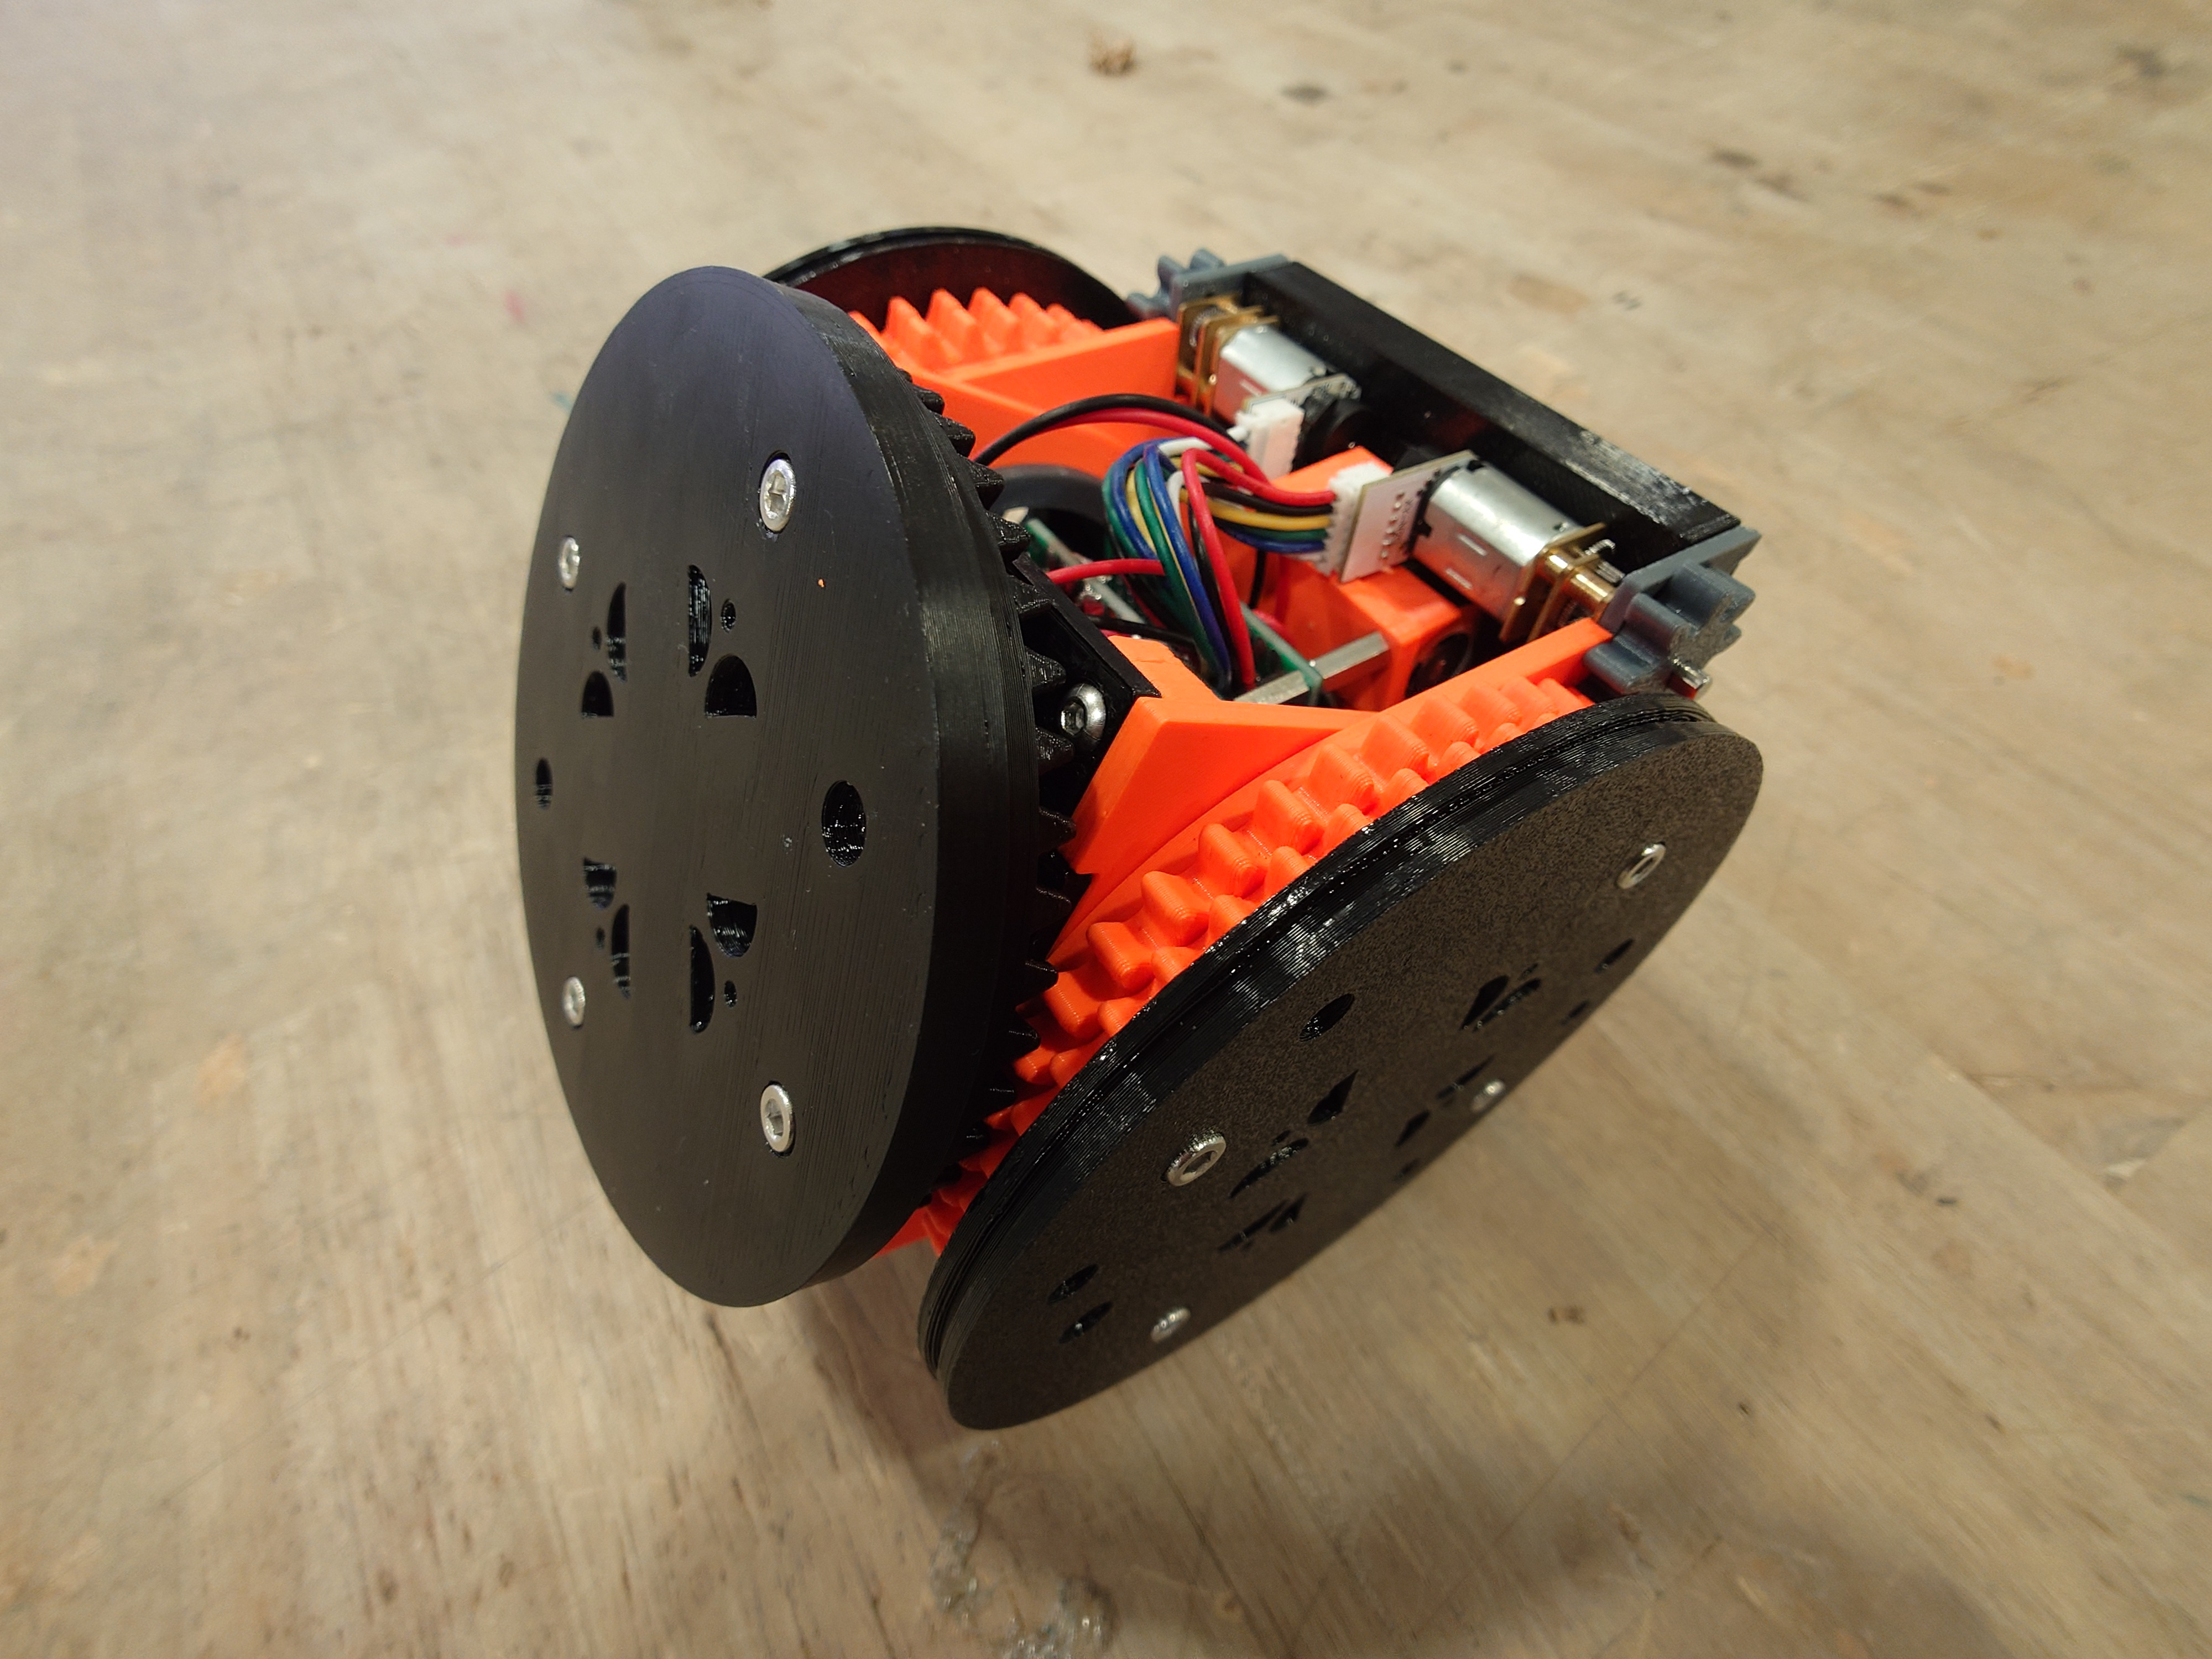
\includegraphics[width=\linewidth,height=3.4cm,keepaspectratio]{../image/assembled_workbench.jpg}
		\caption{Module on the workbench.}
		\label{fig:real-bench}
	\end{subfigure}
	\hfill
	\begin{subfigure}[b]{0.31\textwidth}
		\centering
		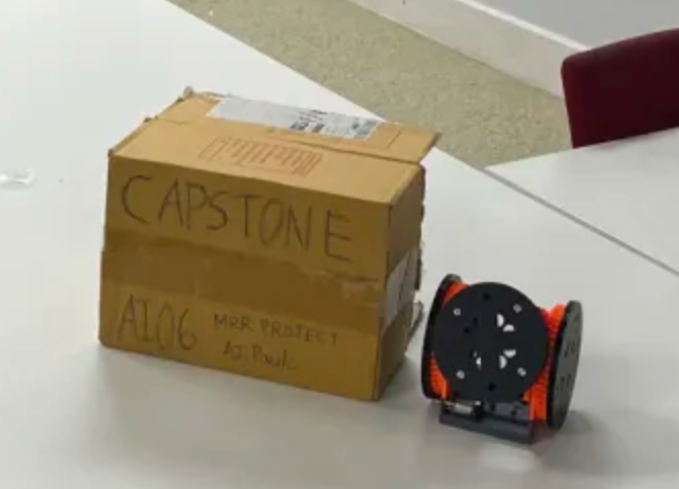
\includegraphics[width=\linewidth,height=3.4cm,keepaspectratio]{../image/assembled_size_reference.png}
		\caption{Module next to a cardboard box for scale.}
		\label{fig:real-size}
	\end{subfigure}
	\caption{Assembled prototype.}
	\label{fig:real-views}
\end{figure}

% ----------------------------------------------------------------
\subsection{Gear Train}
\label{sec:gear-design}

The gear train keeps the SMORES-EP tooth counts (48T spur, 9T pinion, stage ratio $48/9 \approx 5.33{:}1$) and scales the module from $m = 1.4$ to $m = 1.8$, so the spur gear fills the \SI{90}{mm} diameter available inside the envelope. The pan/tilt drive uses a true crown (face) gear instead of the reused spur gear of SMORES-EP. Four motors each drive a pinion: the outer two drive the wheels, and the inner two mesh with the crown gear as a differential (same direction gives tilt, opposite directions give pan). Table~\ref{tab:final-params} lists the final parameters.

\begin{table}[H]
	\centering\small
	\caption{Final gear train parameters.}
	\label{tab:final-params}
	\begin{tabular}{lllllp{4.2cm}}
		\toprule
		\textbf{Component} & \textbf{Teeth} & \textbf{Module} & \textbf{PD} & \textbf{OD} & \textbf{Notes} \\
		\midrule
		Spur gear ($\times$4) & 48 & \num{1.8} & \SI{86.4}{mm} & \SI{90}{mm} &
		\SI{5}{mm} face width \\
		\addlinespace
		Pinion ($\times$4) & 9 & \num{1.8} & \SI{16.2}{mm} & \SI{19.8}{mm} &
		D-bore on the N20 shaft \\
		\addlinespace
		Crown gear & 46 & \num{1.75} & \SI{80.5}{mm} & \SI{84}{mm} &
		True face gear \\
		\bottomrule
	\end{tabular}
\end{table}

\textbf{Status.} All gears have been printed in nylon and tested. Both the spur--pinion and spur--crown meshes turn smoothly. The remaining step is to print test the enlarged pinion D-bore on the motor shaft.

\textbf{Shaft fit.} The \SI{55}{mm} plain bearing acts as the shaft for the wheels, spur gears and tilt joints. A single CAD bore of $\varnothing$\SI{55.15}{mm} (bearing OD $+\SI{0.15}{mm}$) was tested on printed PETG parts and is used for all of them, replacing the separate ISO clearance and interference fits proposed in Progress Report~2.

% ----------------------------------------------------------------
\subsection{Simulation Model}
\label{sec:sim-model}

The module CAD is exported to URDF and simulated in Gazebo Fortress with \texttt{ros2\_control} on ROS~2 Humble. The model has five links (base, two wheels, tilt body, pan face) and four actuated joints: the wheels are velocity controlled by a differential-drive controller, and pan and tilt are position controlled. The link frames were re-aligned with the base following REP-103, and the inertial values were recomputed from the CAD meshes (solid nylon PA12) \cite{mirtich1996}, replacing the exporter's placeholder values.

$N$ identical modules are spawned, each in its own namespace (\texttt{module\_1}, \ldots) with its own controllers, so they can be commanded independently. Each module's exact pose is taken from the physics engine and published as \texttt{/module\_i/ground\_truth/odom}; the AprilTag estimate will later replace this topic without changing the algorithm code. The control package \texttt{msrr\_control} commands all modules from one node, limited to the real top speed of \SI{0.049}{m/s}. A go-to-goal test with three modules reached all goals within \SI{1}{cm}. Docking, gear backlash and the pan/tilt motor coupling are not modelled yet.

\clearpage
% ================================================================
\section{Electronics}
\label{sec:electronics}
% ================================================================

\subsection{Overview and Changes from Progress Report 1}
\label{sec:elec-overview}

The phased plan is unchanged: Phase A-1 uses off-the-shelf boards on a carrier PCB, Phase A moves to custom PCBs, Phase B adds the in-wheel EP-Face circuitry, Phase C adds the ToF camera and Phase D moves compute onboard (Raspberry Pi CM5). The electronics work is one week behind, which shifts the work that depends on it by the same amount.

Two changes were made since Progress Report~1:
\begin{itemize}
  \item \textbf{Phase A-1 parts.} An STM32F411 development board, two TB6612FNG dual H-bridge drivers and an ESP32-C6 replace the COTS 4-channel driver with a built-in MCU and the ESP32-C3. This gives direct control of the PWM, direction and encoder signals, so the wiring and firmware carry over to the Phase A main board.
  \item \textbf{Battery.} The 2S \SI{3000}{mAh} pack is replaced by a 3S pack of Vapcell M11 18350 cells (\SI{1100}{mAh}, \SI{10}{A} continuous). It can supply more current for the EP-Face in Phase B, at the cost of run time (Section~\ref{sec:power-new}).
\end{itemize}

% ----------------------------------------------------------------
\subsection{Phase A-1: Carrier Board (First Iteration)}
\label{sec:phase-a1-hw}

The A-1 module board is a carrier PCB with \SI{2.54}{mm} sockets and no SMT parts, which replaces the bench wiring (Figure~\ref{fig:a1-mod-pcb}). It carries a Black Pill STM32F411, two TB6612FNG driver modules, a \SI{5}{V} buck module, an ESP32-C6 Zero for Wi-Fi and a small UWB breakout (Ai-Thinker BU01, DW1000). The drivers run directly from the pack. The STM32F411 runs at \SI{96}{MHz}, with \SI{20}{kHz} motor PWM, one quadrature timer per encoder and a \SI{1}{kHz} control-loop tick; its pin map is given in the firmware section (Table~\ref{pr3:tab:pins}). With the PR1 load figures, the A-1 set-up draws \SI{3.3}{W} typical from the pack (about \SI{3}{h} run time) and \SI{2.7}{A} at worst case, well inside the cells' rating.

Inside the module, the boards stand upright, parallel to the tilt face, with the three cells in a column at the back so that the heaviest part sits close to the wheel axis (Figure~\ref{fig:a1-electronics-section}).

\begin{figure}[!htbp]
  \centering
  \begin{subfigure}[b]{0.38\textwidth}
    \centering
    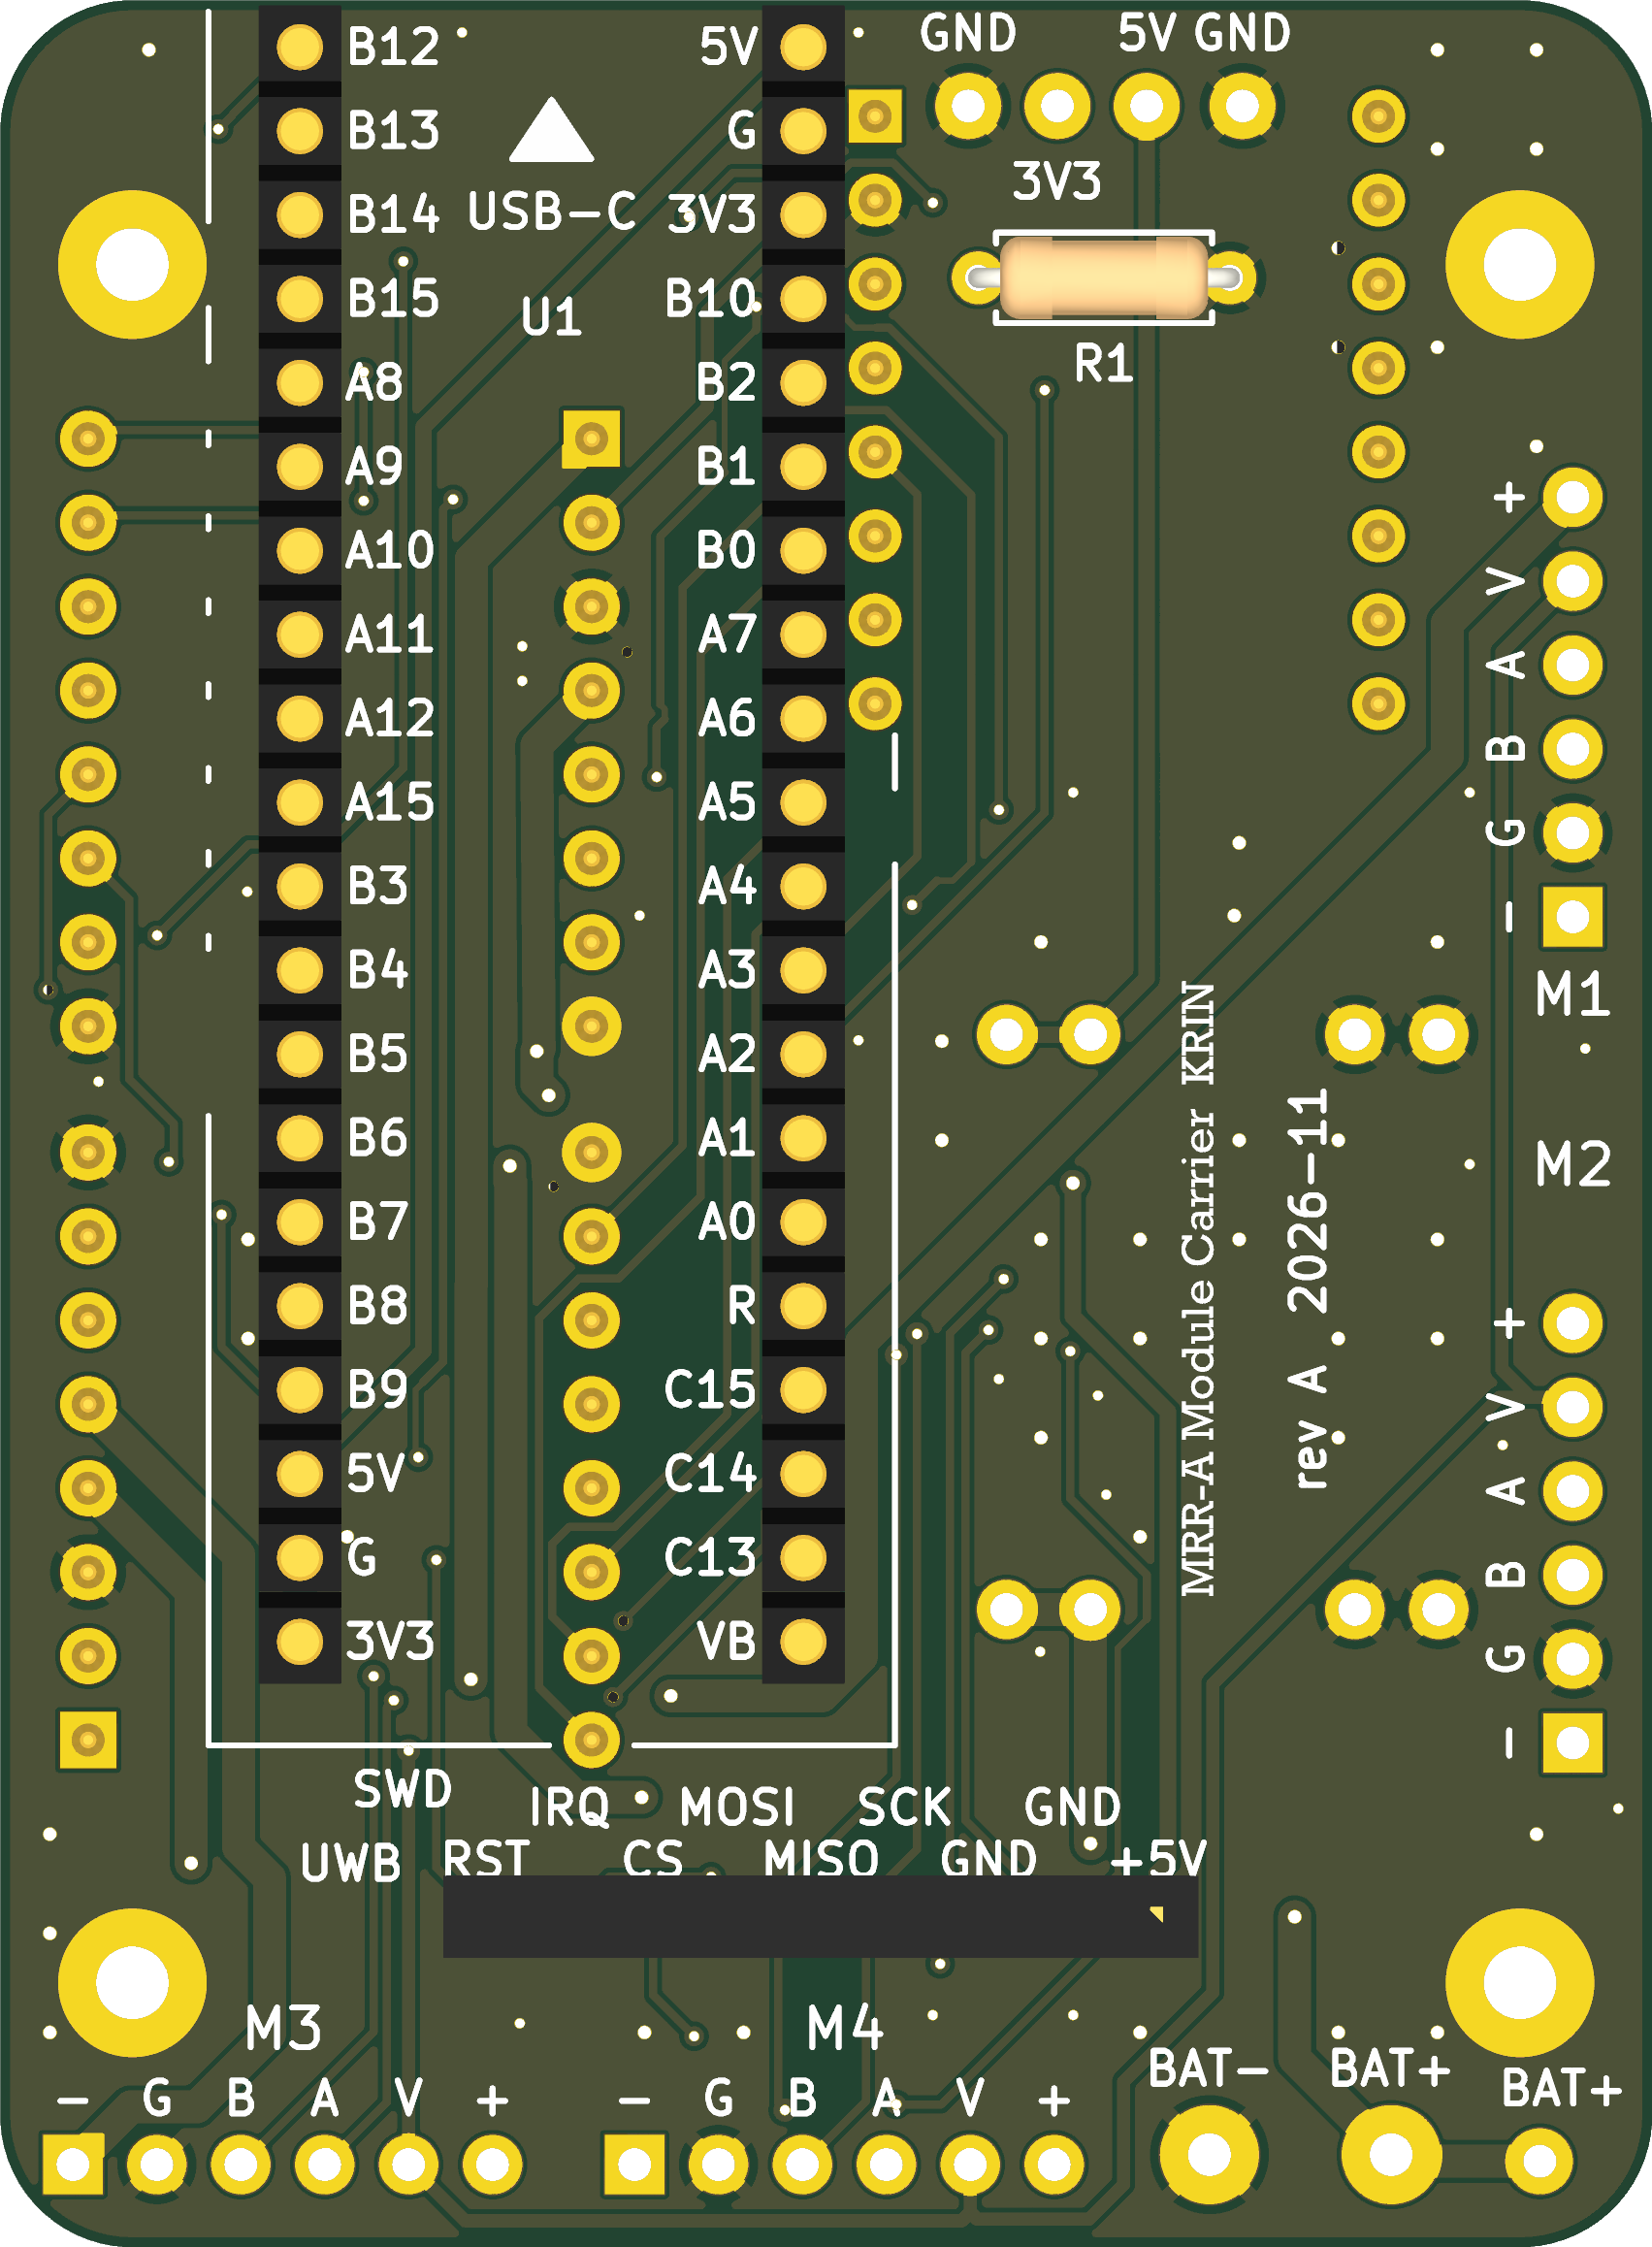
\includegraphics[width=\linewidth]{../image/PhaseA1_Board_Module_Top.png}
    \caption{Top.}
  \end{subfigure}
  \hfill
  \begin{subfigure}[b]{0.38\textwidth}
    \centering
    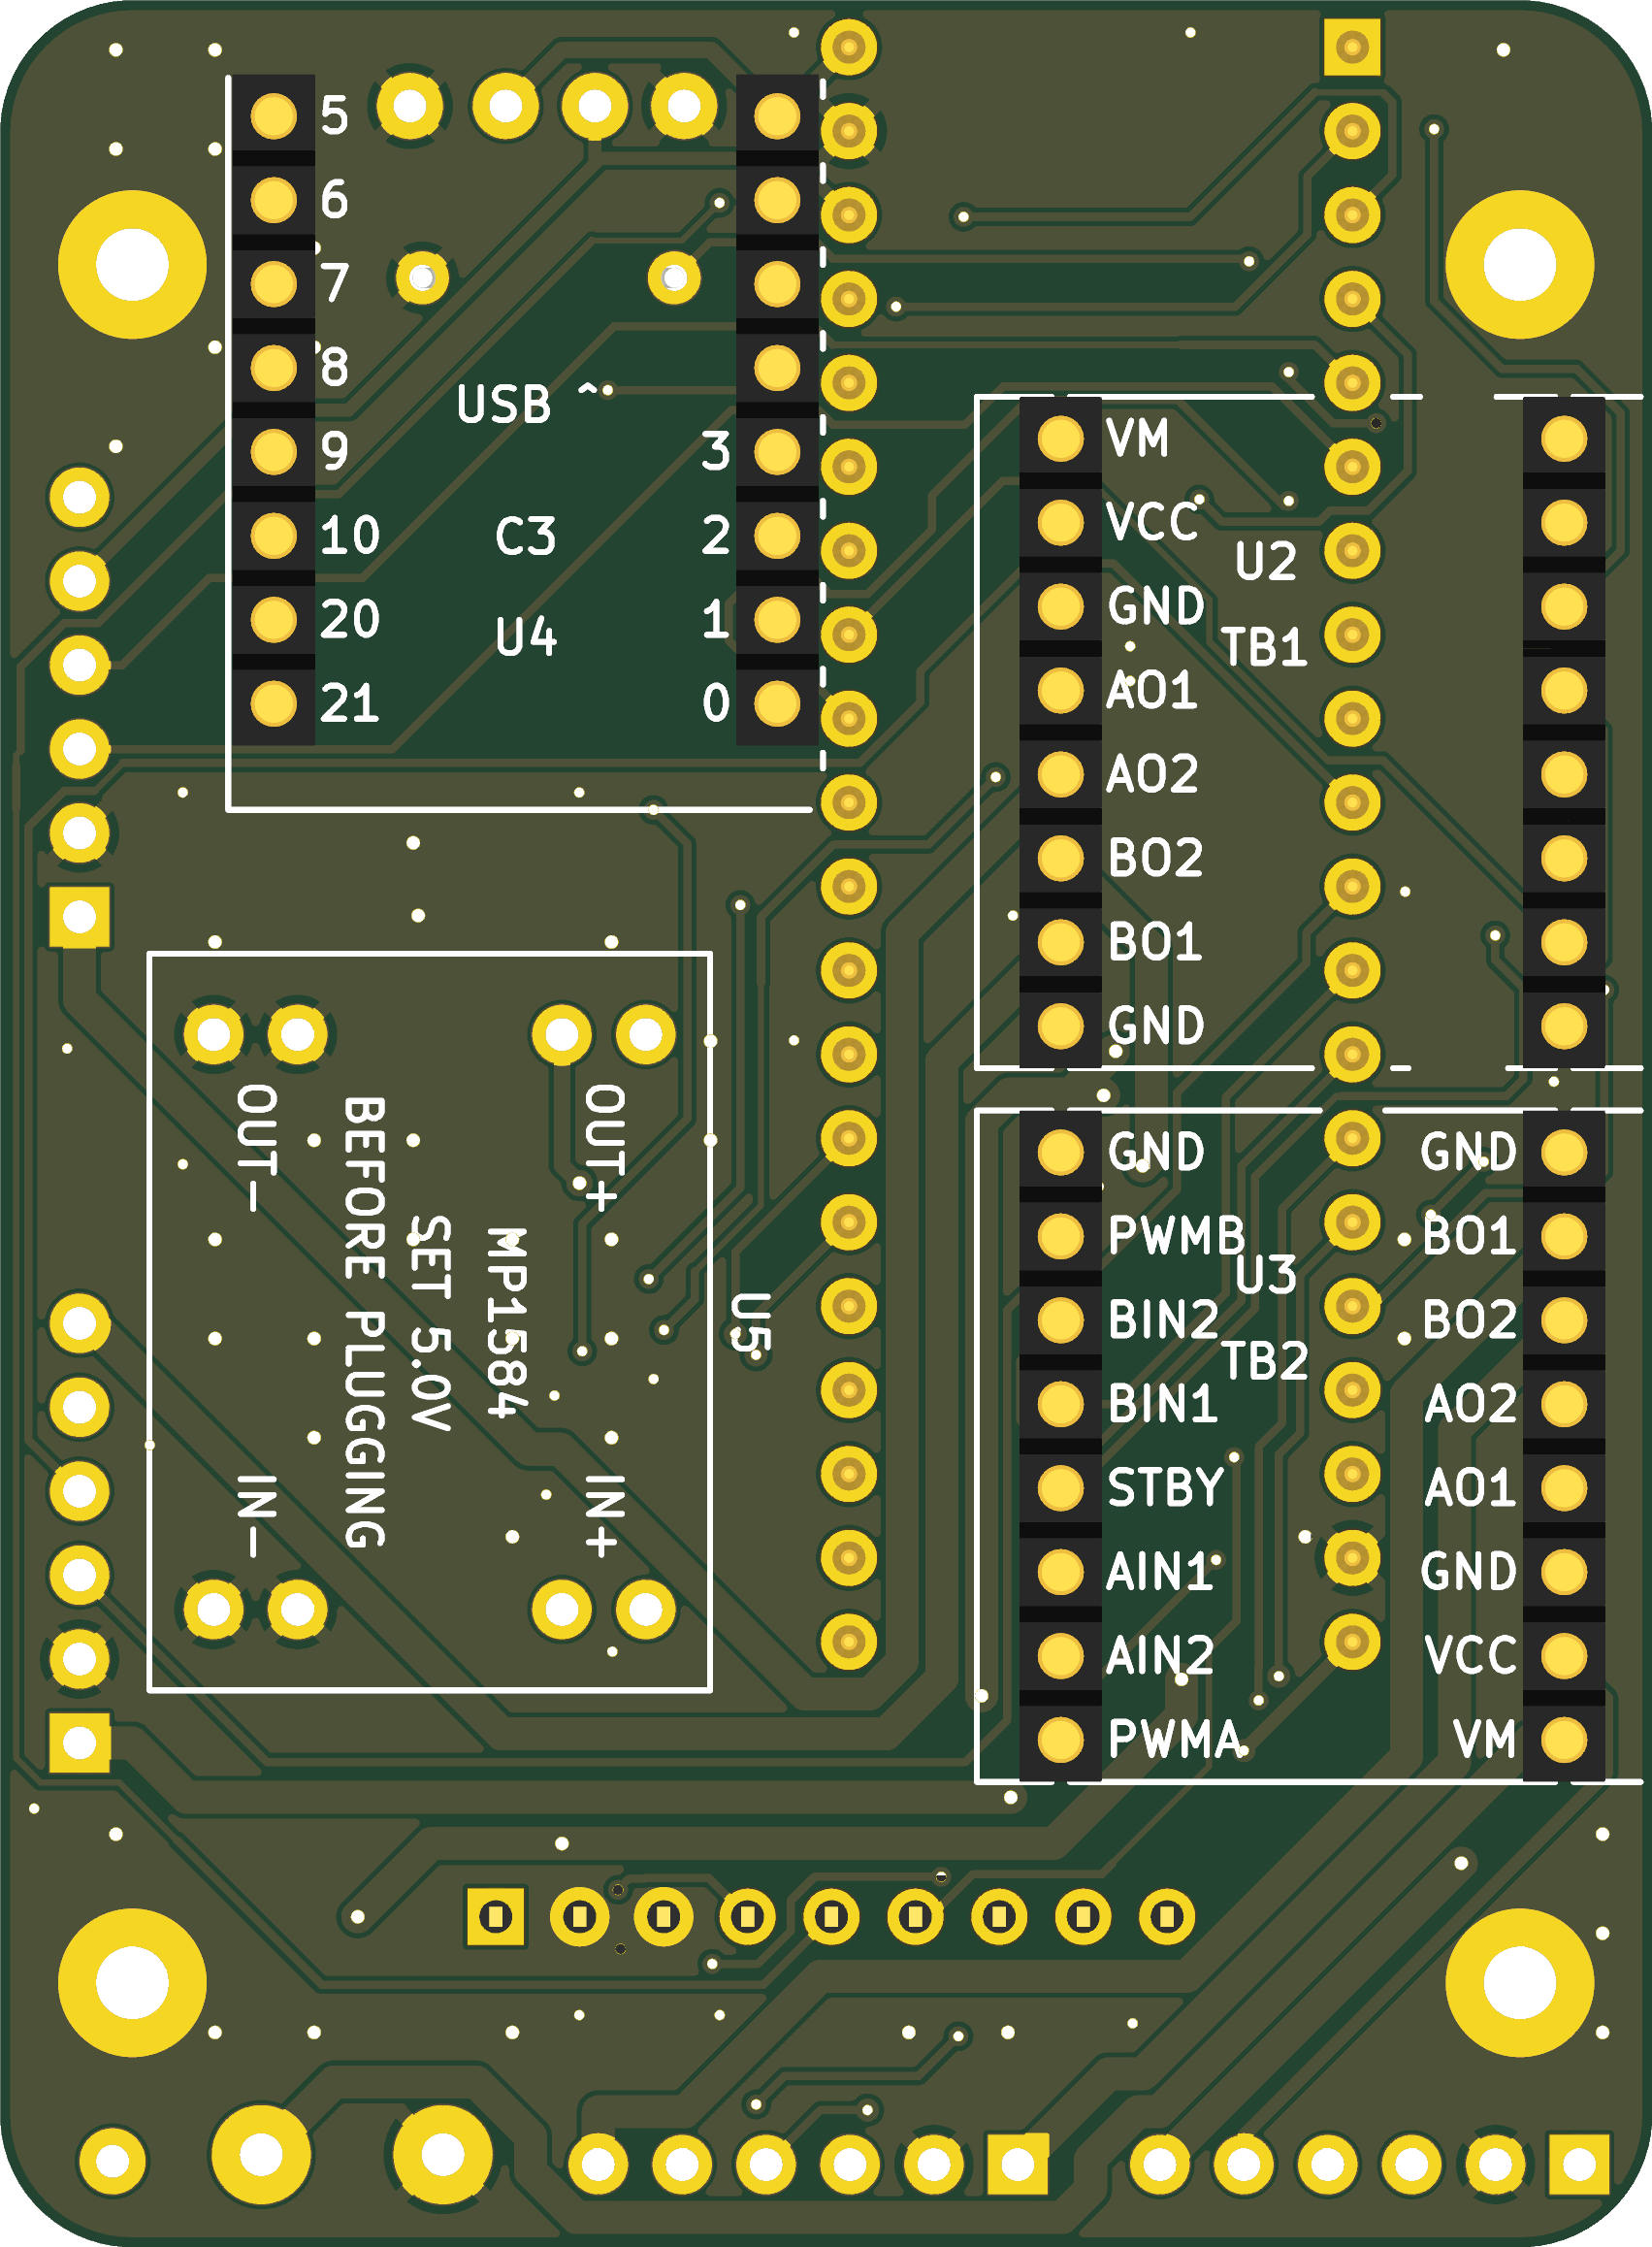
\includegraphics[width=\linewidth]{../image/PhaseA1_Board_Module_Bottom.png}
    \caption{Bottom.}
  \end{subfigure}
  \caption{A-1 module board PCB render.}
  \label{fig:a1-mod-pcb}
\end{figure}

\begin{figure}[!htbp]
  \centering
  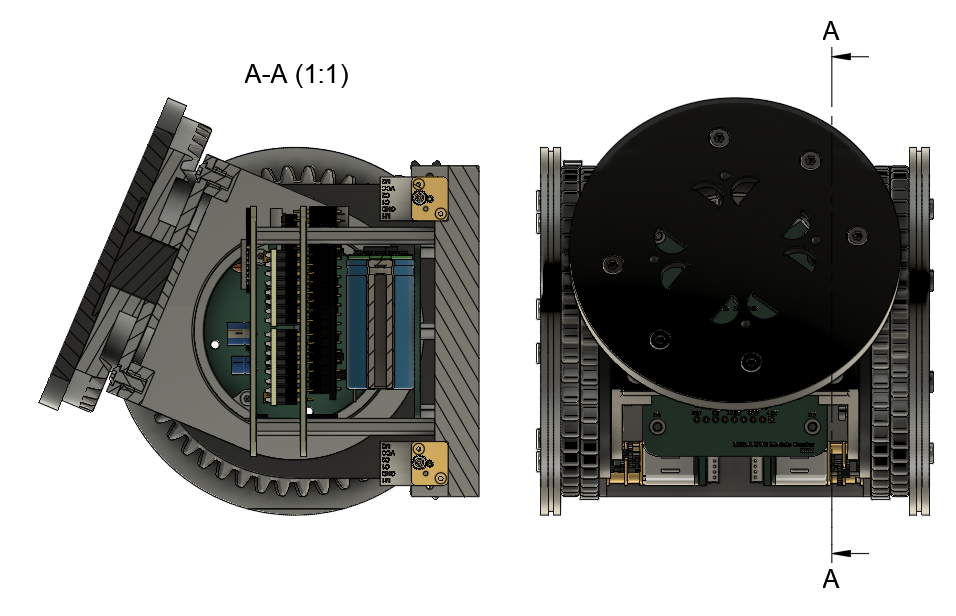
\includegraphics[width=0.75\textwidth]{../image/Electronics_in_the_assembly.png}
  \caption{Sectional view (A-A) of the electronics inside the MRR module: carrier board with plug-in modules, and the 18350 cell column at the back.}
  \label{fig:a1-electronics-section}
\end{figure}

% ----------------------------------------------------------------
\subsection{Phase A: Power Architecture (Second Iteration)}
\label{sec:power-new}

The Phase A power design keeps the PR1 architecture: the H-bridges run directly from the pack (PWM capped at about \SI{48}{\percent} for the \SI{6}{V} motors), a dedicated buck regulator feeds the EP-Face so its pulses do not reach the logic rail, and the logic uses a \SI{5}{V} buck and a \SI{3.3}{V} LDO (Figure~\ref{fig:power-diagram}). Table~\ref{tab:battery-change} compares the two packs. Run time roughly halves, which is acceptable for lab testing in Phases A--C. The higher pack voltage requires H-bridges rated above \SI{12.6}{V} and \SI{2.1}{A} per channel, and buck regulators with a \SIrange{9}{12.6}{V} input.

\begin{figure}[!htbp]
  \centering
  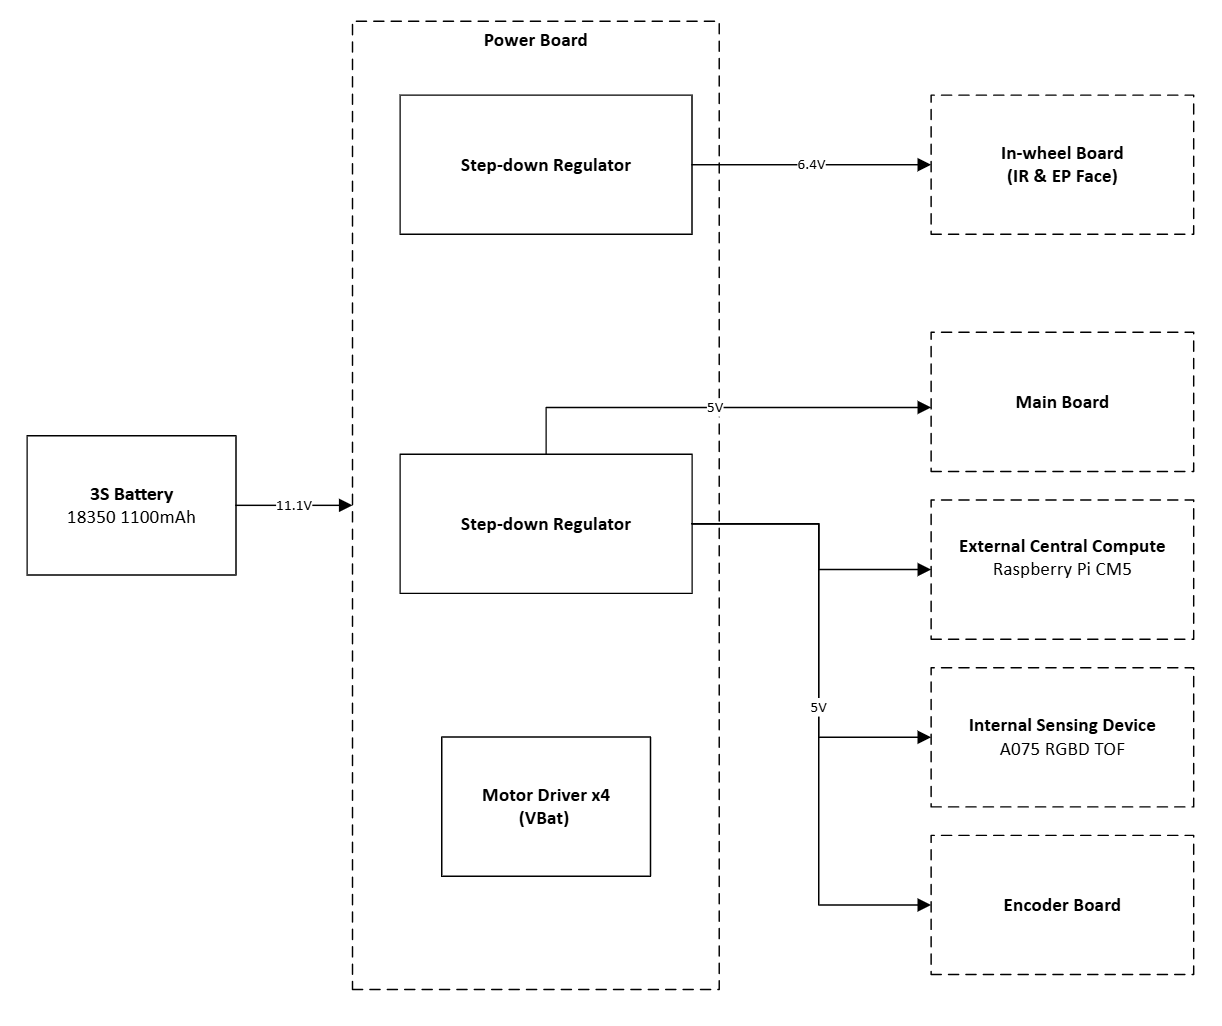
\includegraphics[width=0.55\textwidth]{../image/Power_Diagram.png}
  \caption{Power distribution block diagram.}
  \label{fig:power-diagram}
\end{figure}

\begin{table}[H]
\centering\small
\caption{Battery comparison, PR1 vs.\ PR2 (80\,\% of energy usable).}
\label{tab:battery-change}
\begin{tabular}{@{}lcc@{}}
\toprule
 & \textbf{PR1: 2S 505080} & \textbf{PR2: 3S Vapcell M11} \\
\midrule
Voltage (nominal / full / cutoff) & 7.4 / 8.4 / 6.6\,V & 11.1 / 12.6 / 9.0\,V \\
Capacity / energy (usable) & 3000\,mAh / 22.2\,Wh (17.8) & 1100\,mAh / 12.2\,Wh (9.8) \\
Run time, Phase A--B ($\sim$3.1\,W) & 5.8\,h & \textbf{3.2\,h} \\
Run time, Phase D ($\sim$11.5\,W) & 1.5\,h & \textbf{0.85\,h} \\
Peak current ($\sim$47\,W) & 7.1\,A (2.4\,C) & 5.2\,A (4.7\,C, cell rated 10\,A) \\
\bottomrule
\end{tabular}
\end{table}

% ----------------------------------------------------------------
\subsection{Phase A: Main and Communication Boards (Second Iteration)}
\label{sec:phase-a-board}

The Phase A electronics are two stacked boards that replace the A-1 carrier (Table~\ref{tab:a-board-summary}). The \emph{main board} (MRR\_A) carries the STM32G474 controller, four DRV8876 H-bridges with current sensing, the IMU, the battery charger and the power tree. The \emph{communication board} (MRR\_A\_RF) carries the ESP32-C6 Wi-Fi module and the DWM3000 UWB module. It sits on top of the stack so the antennas are clear of the metal, and all signals cross a 2$\times$8 header. The schematic is hierarchical (Figure~\ref{fig:a-sch-main-root}). The STM32G474 runs at \SI{170}{MHz}; the motor PWM timer triggers the ADC so the current samples line up with the PWM, and each encoder has its own quadrature timer. Figures~\ref{fig:a-pcb-main} and~\ref{fig:a-pcb-comm} show the PCB renders. The full schematic sheets, pin map and CubeMX configuration are in the full report.

\begin{table}[H]
\centering\small
\caption{Phase A board summary.}
\label{tab:a-board-summary}
\begin{tabular}{@{}L{0.22\textwidth} L{0.34\textwidth} L{0.34\textwidth}@{}}
\toprule
 & \textbf{Main board (MRR\_A)} & \textbf{Comm.\ board (MRR\_A\_RF)} \\
\midrule
Controller & STM32G474RET6 (Cortex-M4F, 170\,MHz) & ESP32-C6-MINI-1U \\
Motor drive & 4$\times$ DRV8876PWPR, PH/EN mode, IPROPI current output & -- \\
Sensors / radio & ICM-42605 IMU (SPI) & DWM3000 UWB (SPI) \\
Power & 3S input, e-fuse TPS259830L, buck TPS62933F (5\,V), LDO TPS7A9101 (3.3\,V), BQ25798 charger & 3.3\,V from the main board \\
Communication & USB-C, FDCAN (500\,kbit/s), UART to ESP32-C6 & USB-C, UART header \\
Size / layers & 68$\times$50\,mm, 4 layers & 68$\times$50\,mm, 4 layers \\
\bottomrule
\end{tabular}
\end{table}

\begin{figure}[!htbp]
  \centering
  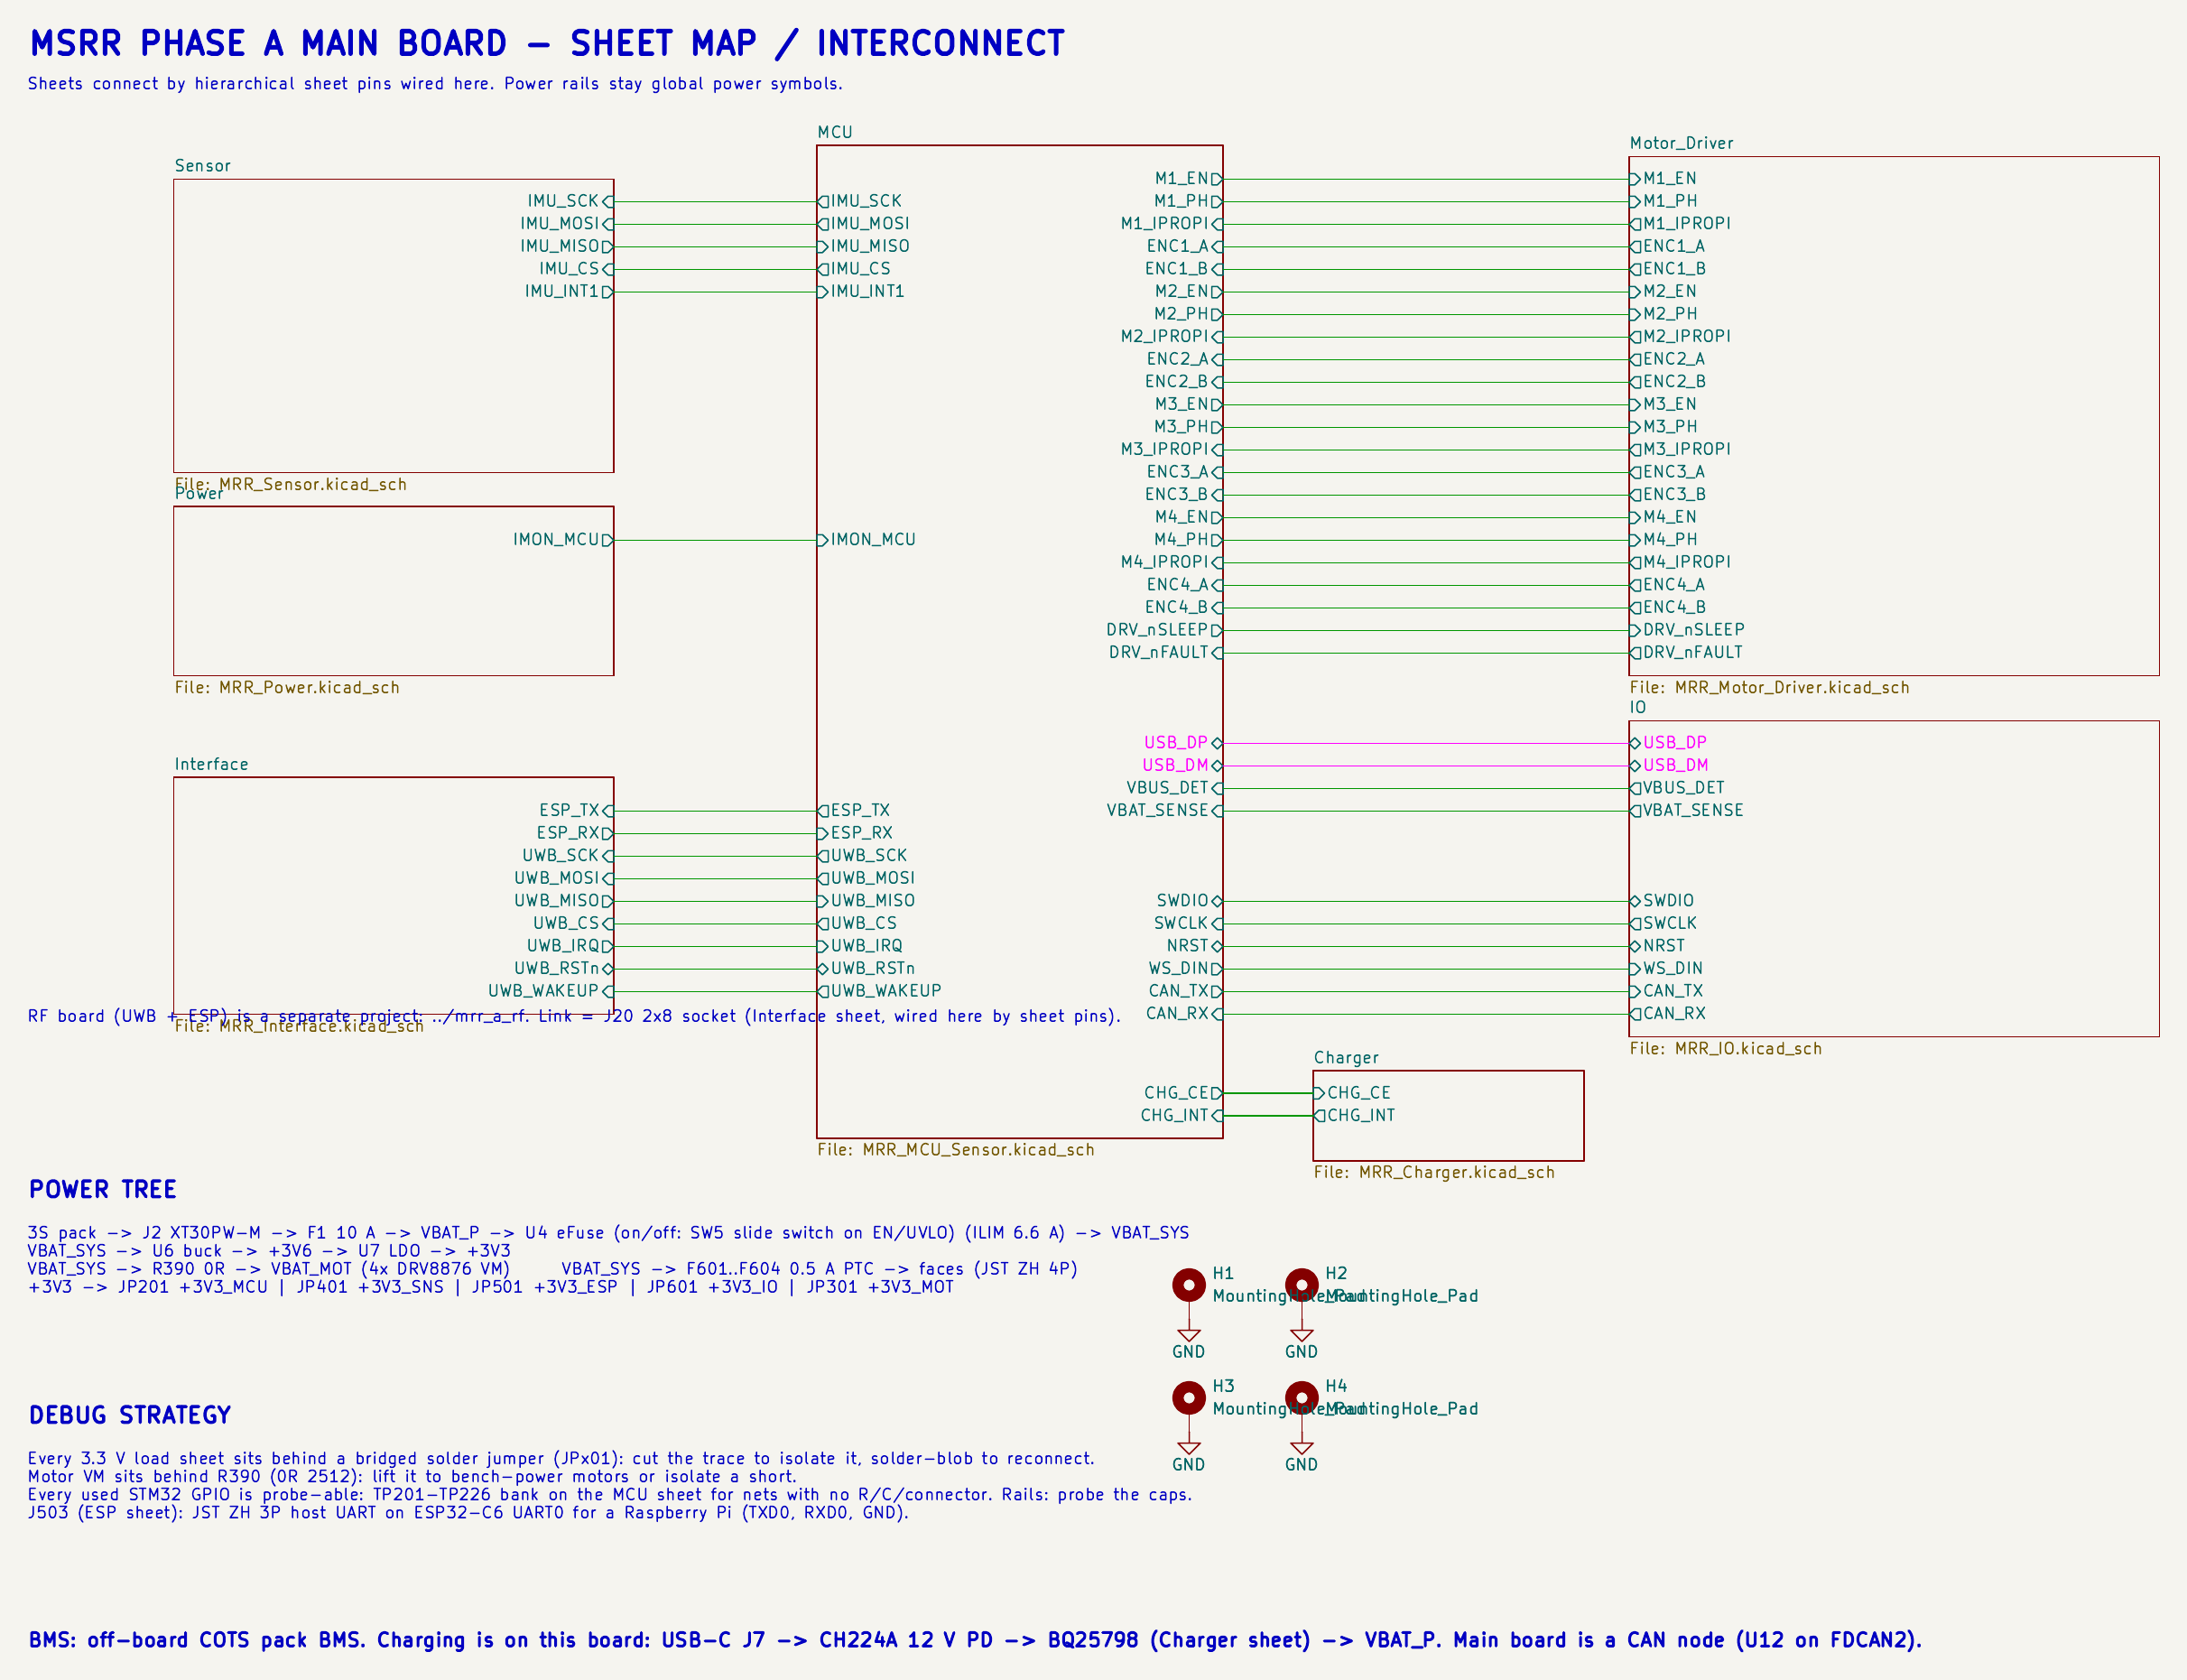
\includegraphics[width=0.75\textwidth]{../image/PhaseA_Sch_Main_Root.png}
  \caption{Main board schematic: sheet map.}
  \label{fig:a-sch-main-root}
\end{figure}

\begin{figure}[!htbp]
  \centering
  \begin{subfigure}[b]{0.38\textwidth}
    \centering
    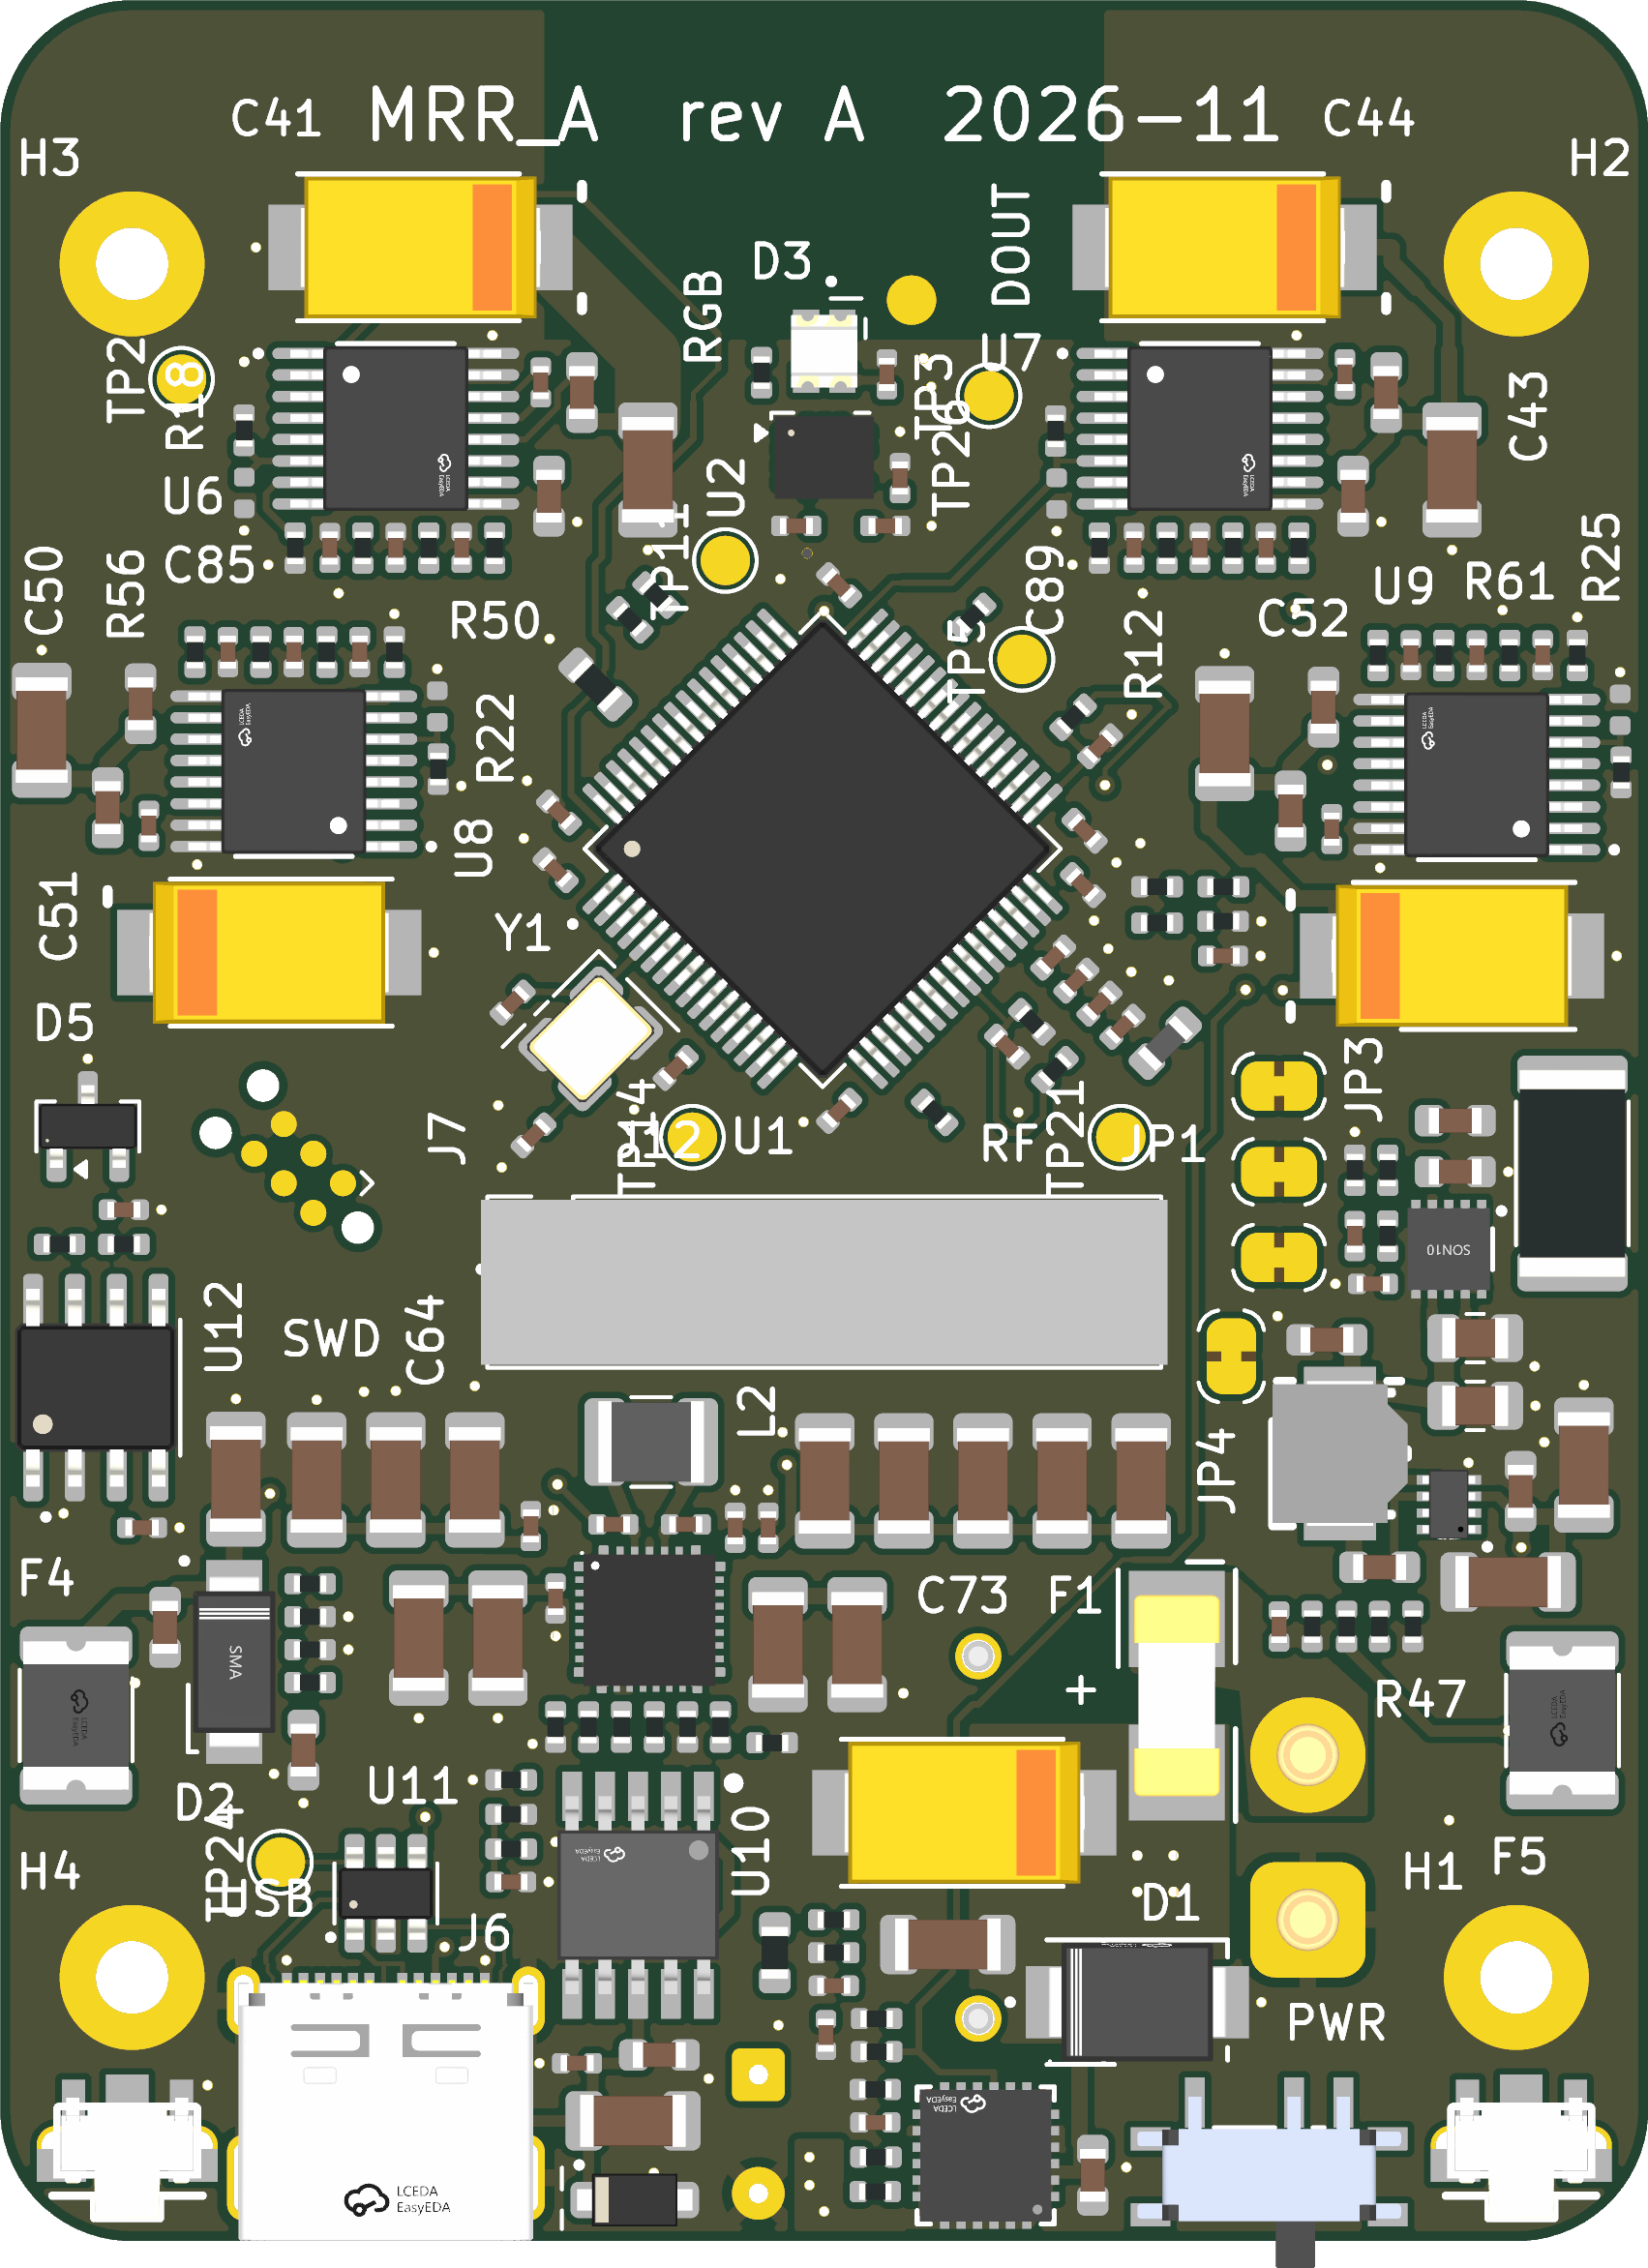
\includegraphics[width=\linewidth]{../image/PhaseA_Board_Main_Top.png}
    \caption{Top.}
  \end{subfigure}
  \hfill
  \begin{subfigure}[b]{0.38\textwidth}
    \centering
    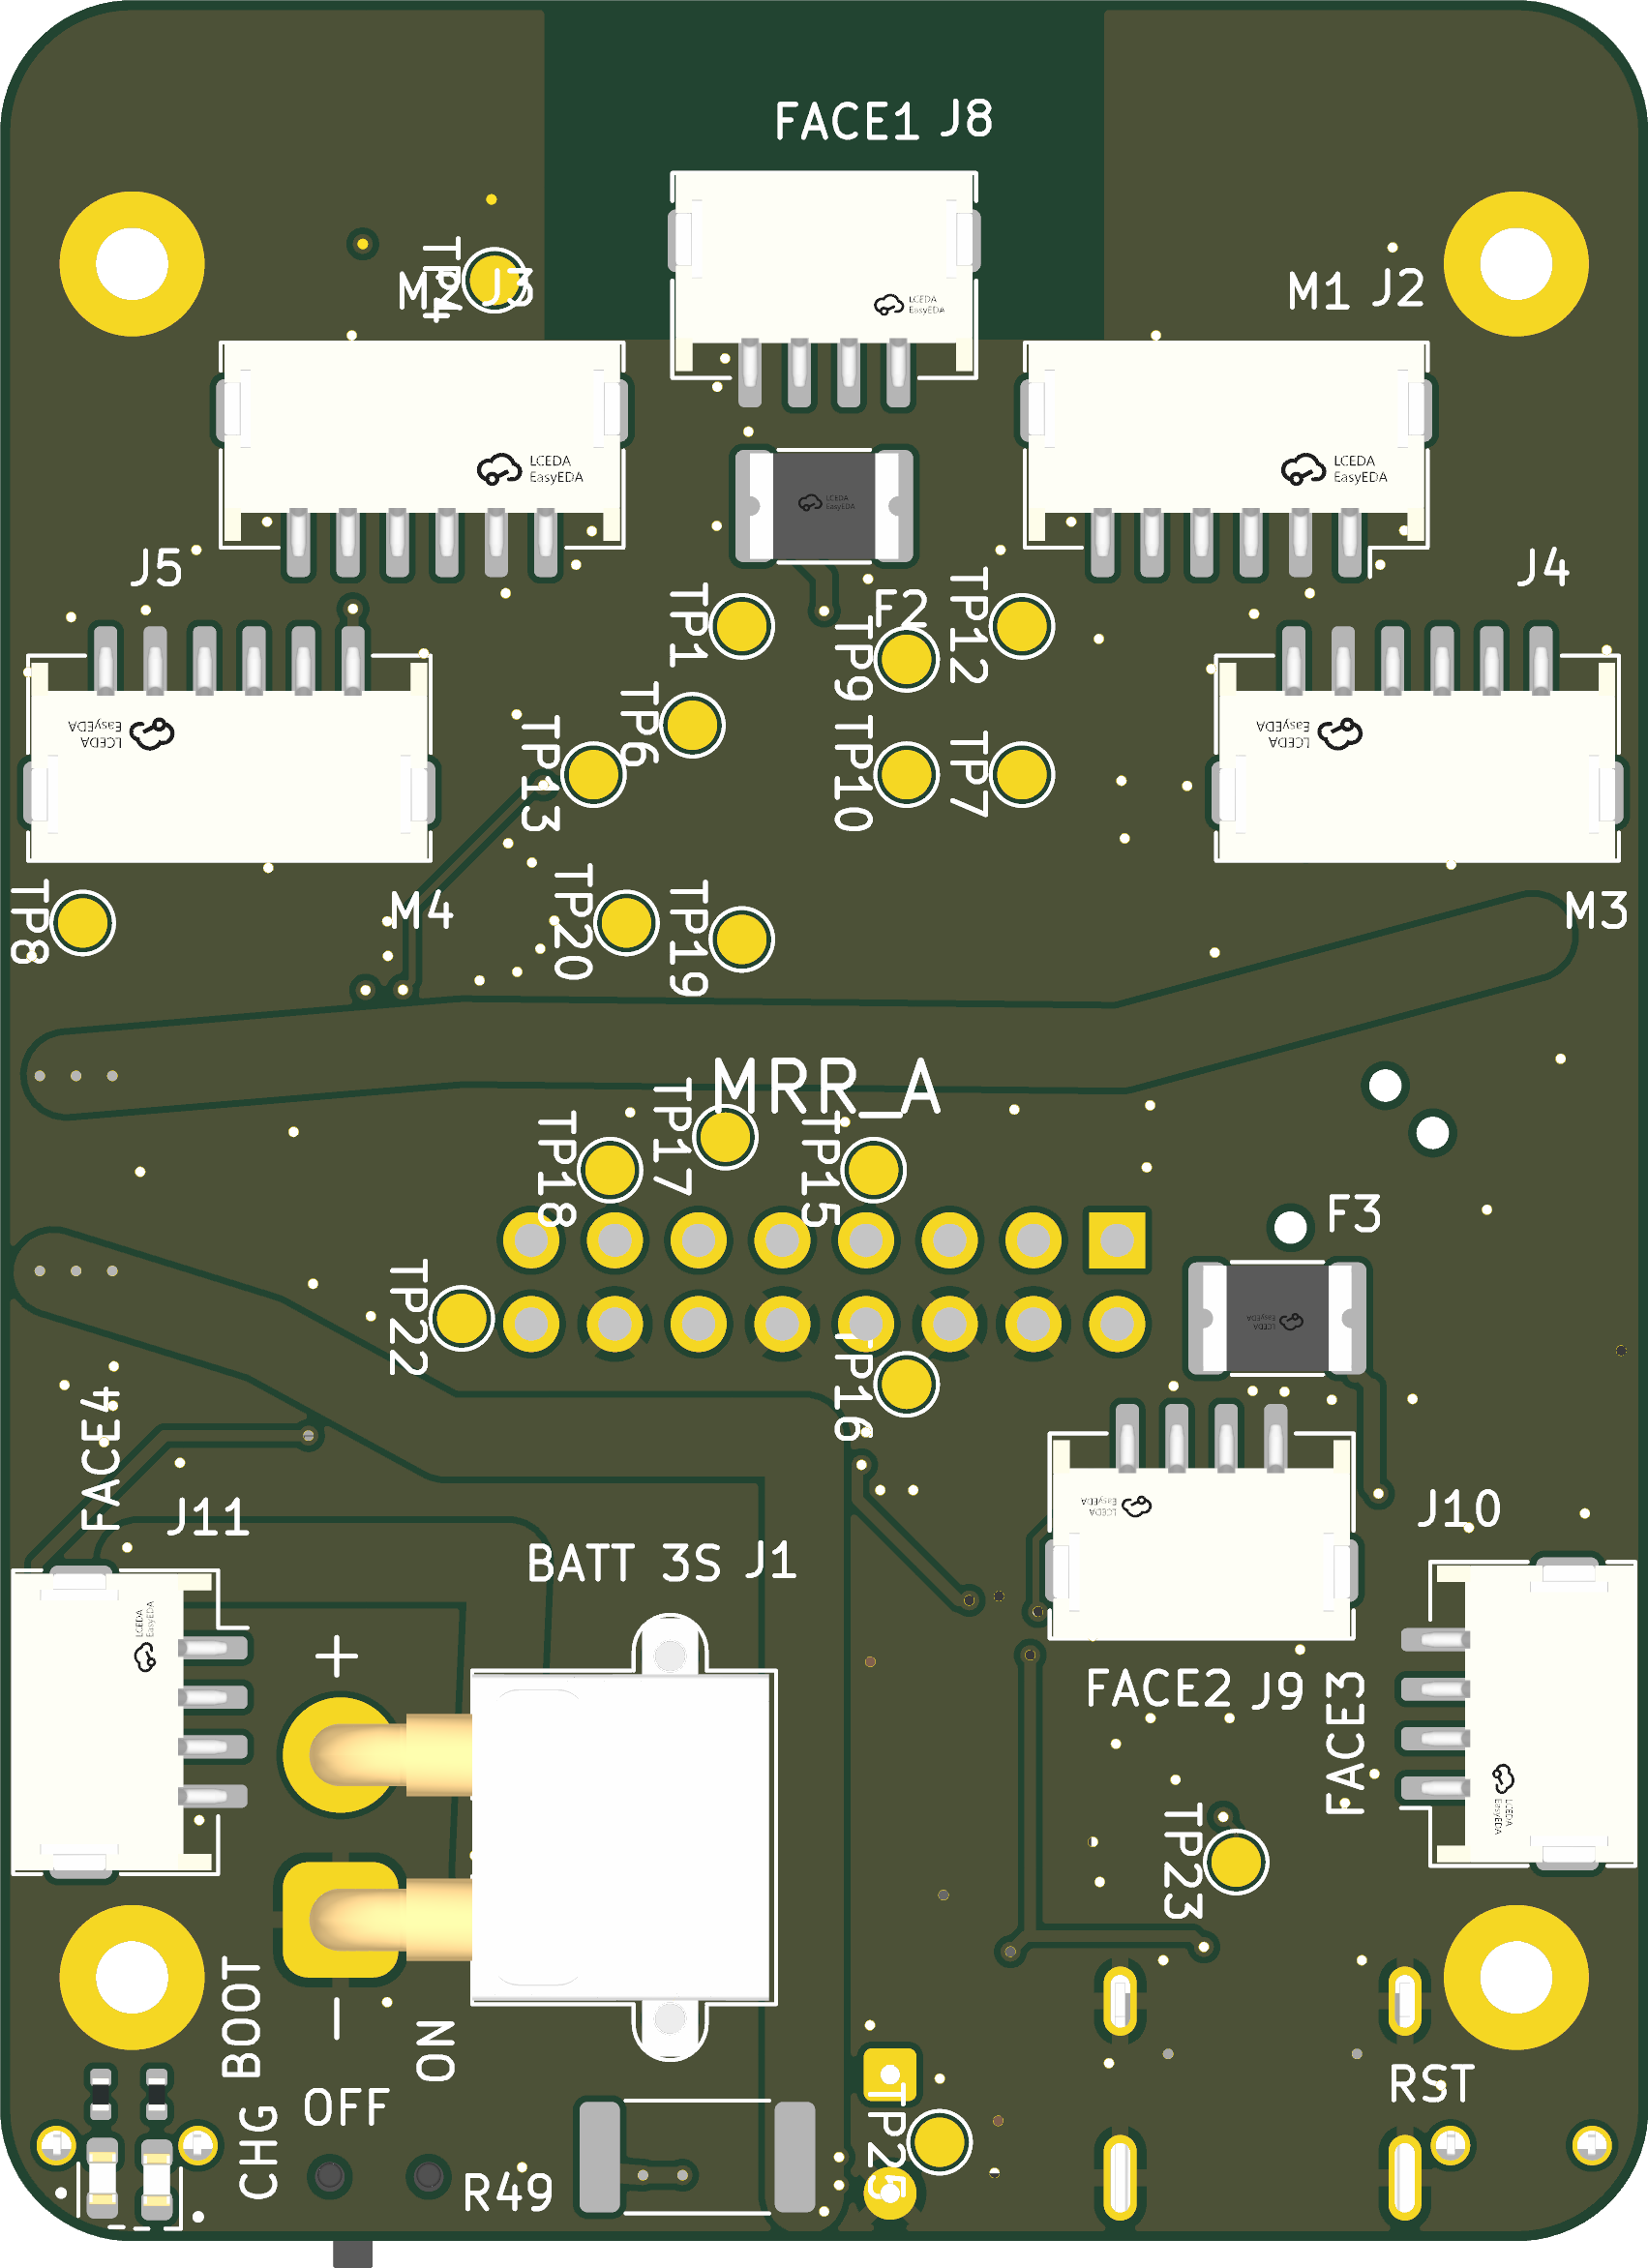
\includegraphics[width=\linewidth]{../image/PhaseA_Board_Main_Bottom.png}
    \caption{Bottom.}
  \end{subfigure}
  \caption{Main board (MRR\_A) PCB render.}
  \label{fig:a-pcb-main}
\end{figure}

\begin{figure}[!htbp]
  \centering
  \begin{subfigure}[b]{0.38\textwidth}
    \centering
    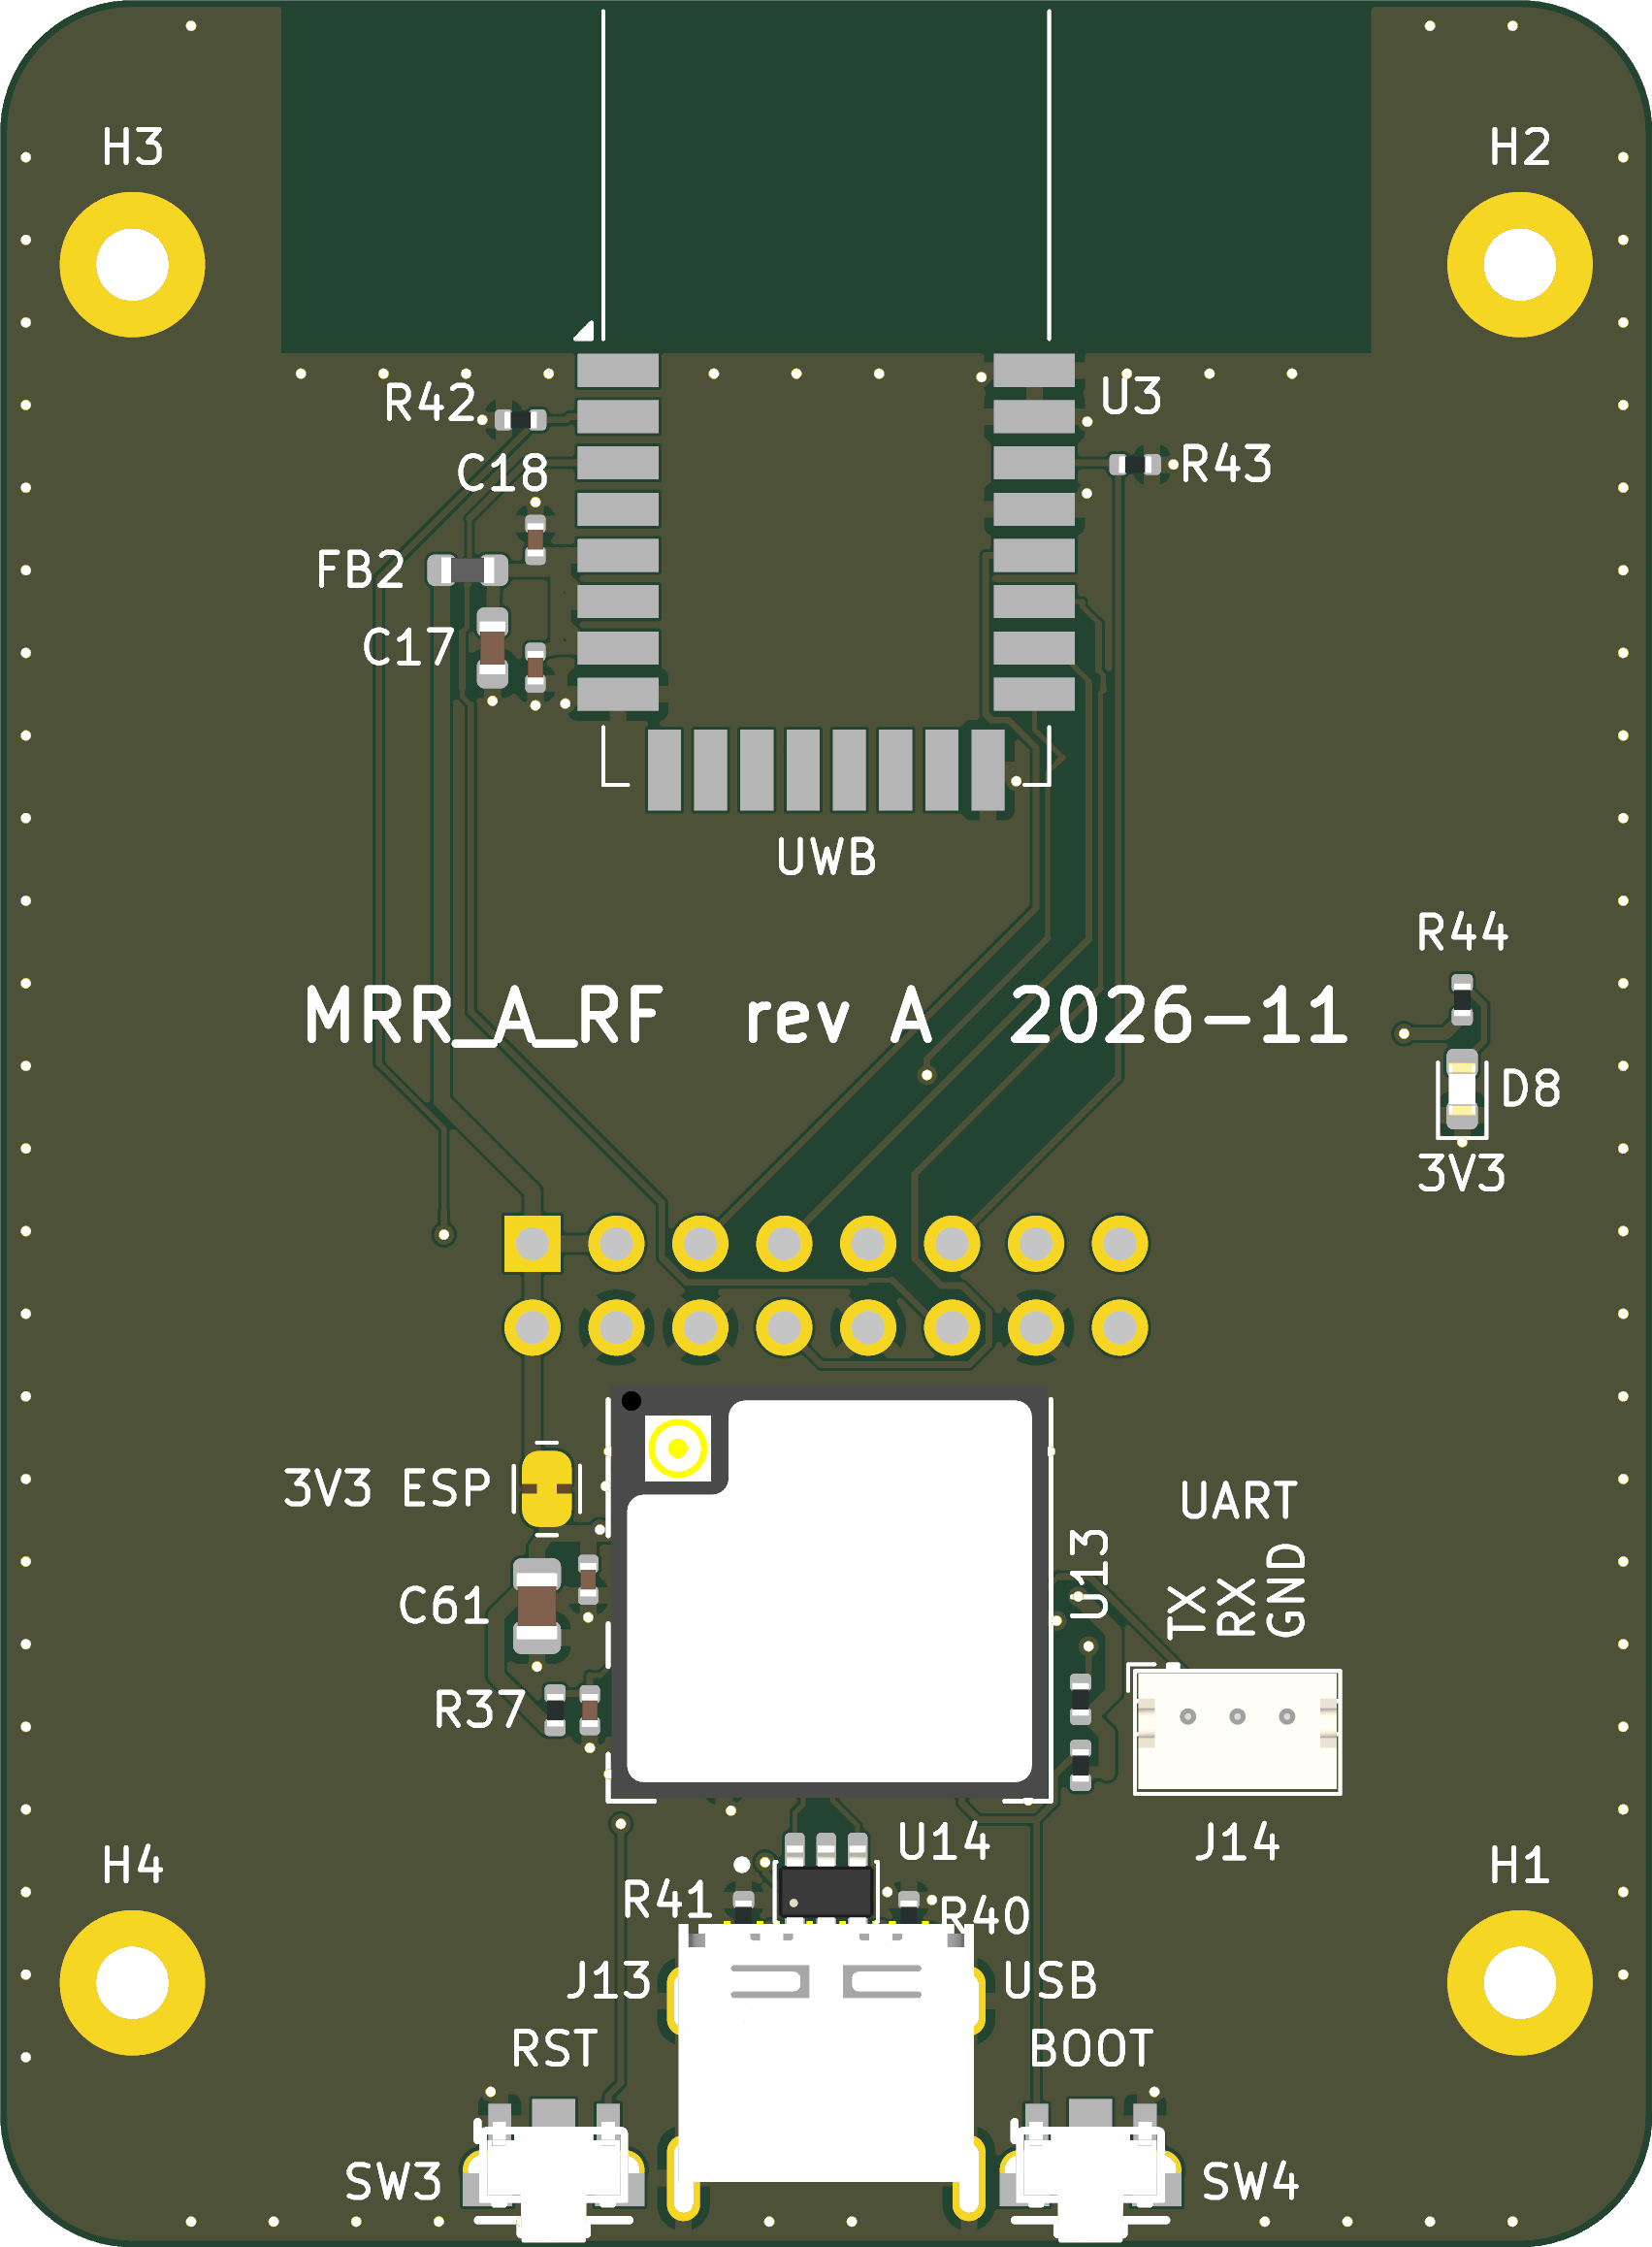
\includegraphics[width=\linewidth]{../image/PhaseA_Board_Comm_Top.png}
    \caption{Top.}
  \end{subfigure}
  \hfill
  \begin{subfigure}[b]{0.38\textwidth}
    \centering
    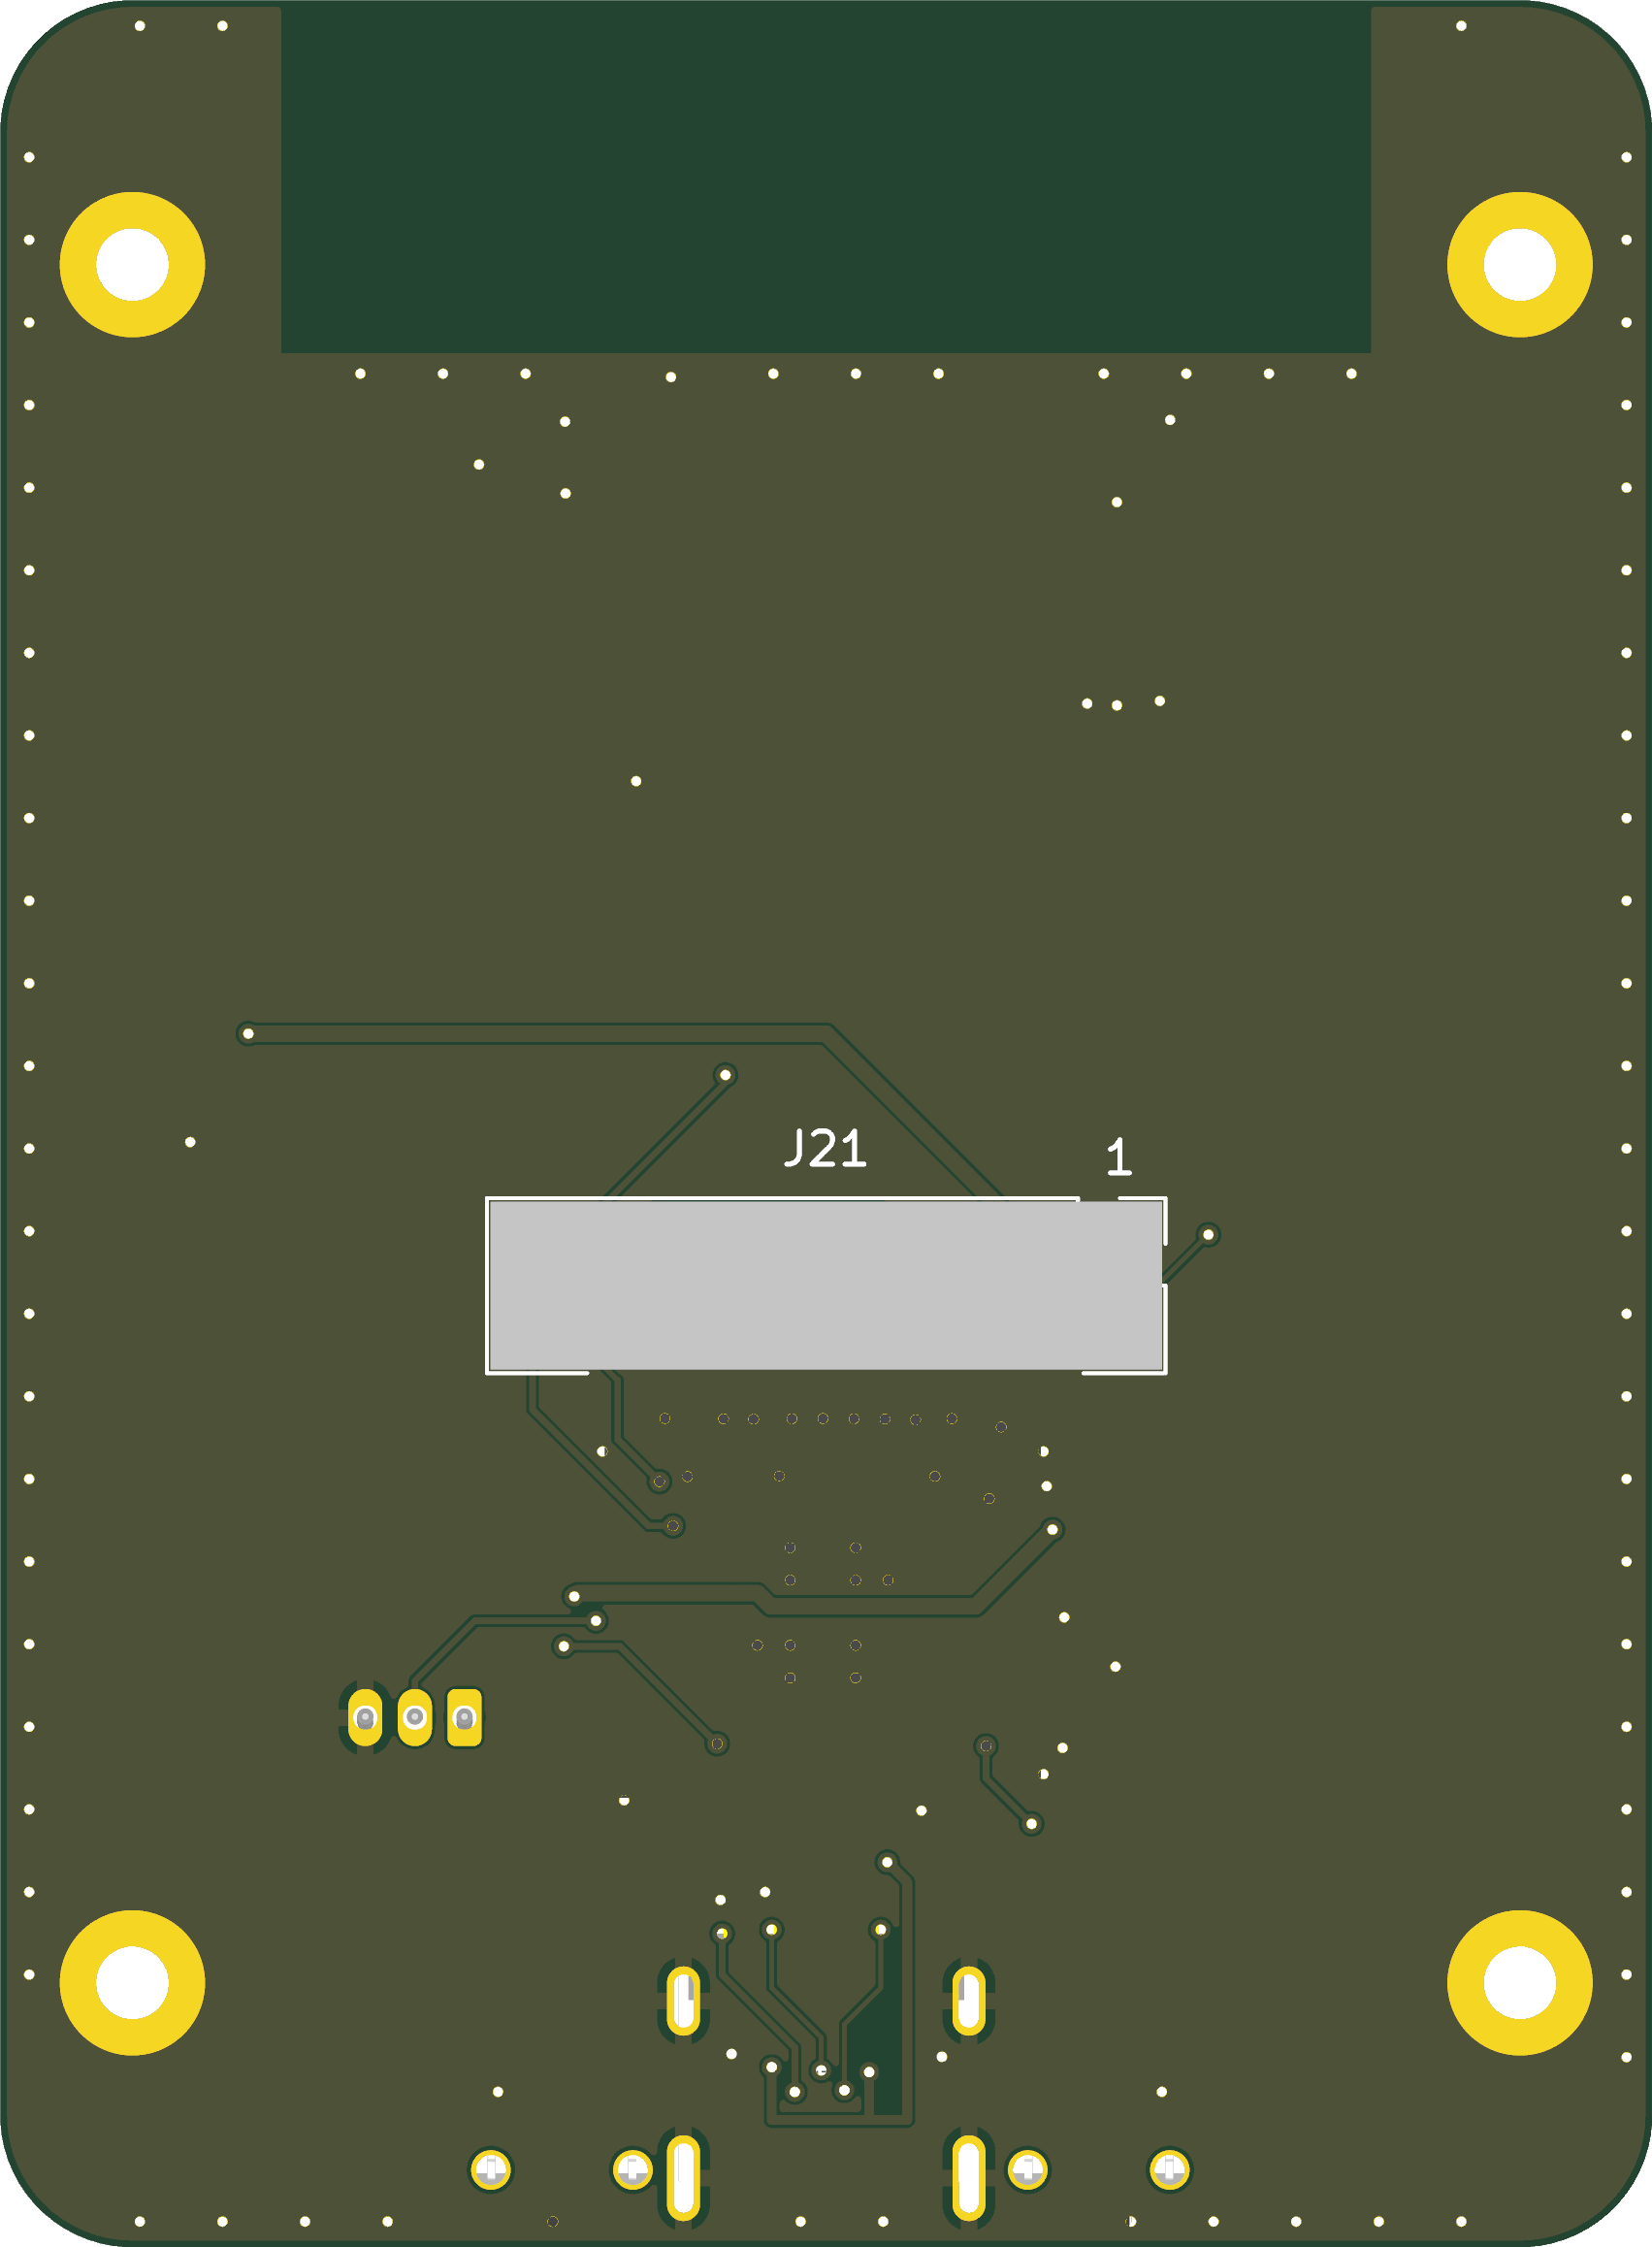
\includegraphics[width=\linewidth]{../image/PhaseA_Board_Comm_Bottom.png}
    \caption{Bottom.}
  \end{subfigure}
  \caption{Communication board (MRR\_A\_RF) PCB render.}
  \label{fig:a-pcb-comm}
\end{figure}

Phases B to D are planned and their hardware is not built yet.

\clearpage
% ================================================================
\section{Teleoperation Architecture}
\label{sec:teleop-architecture}
% ================================================================

Since Progress Report 2 the teleoperation stack has been brought up on the real module, and
the module now drives on its wheels from ROS~2 velocity commands. The PC--module link was
changed from the planned custom \texttt{ros2\_control} plugin with a UDP bridge to
micro-ROS \cite{microros}, the kinematics moved onto the module's ESP32-C6, and the STM32F411
firmware was completed for all four motors. Figure~\ref{fig:teleop-architecture} shows the
new architecture, which replaces the PR2 architecture figure. The subsections below describe
both firmwares and the test results.

\subsection{Changes from Progress Report 2}

Table~\ref{pr3:tab:changes} lists the changes made to the embedded design since PR2.
The hardware (STM32F411 board, two TB6612FNG drivers, ESP32-C6, four N20 gearmotors)
is unchanged. The changes are in the software architecture and in corrections found
during bring-up.

\begin{table}[H]
\centering
\caption{Embedded-system changes from PR2 to PR3.}
\label{pr3:tab:changes}
\small
\begin{tabularx}{\linewidth}{>{\raggedright\arraybackslash}p{3.0cm} >{\raggedright\arraybackslash}X >{\raggedright\arraybackslash}X}
\toprule
Item & PR2 & PR3 (current) \\
\midrule
PC--module link &
  Custom \texttt{ros2\_control} plugin (\texttt{mrr\_hardware}) packs wheel targets into UDP packets;
  the ESP32 is a transparent Wi-Fi$\leftrightarrow$UART bridge. &
  \textbf{micro-ROS}: the ESP32-C6 is a ROS~2 node that talks to a micro-ROS agent on the PC
  (Wi-Fi, UDP). \\
Where kinematics run &
  PC (\texttt{diff\_drive\_controller}). &
  ESP32-C6 on each module (wheel IK/FK and pan/tilt mixing). \\
Low-level control &
  Wheel speed PID only (M1, M2). &
  All four motors; cascaded position/velocity control; four modes. \\
Motor numbering &
  M1, M2 = wheels; M3, M4 = inner (pan/tilt). &
  M3\_L, M4\_R = wheels; M1\_iL, M2\_iR = inner spur gears (Table~\ref{pr3:tab:pins}). \\
Driver standby pin &
  PB10. &
  \textbf{PC15} (checked on the wired board). \\
Wheel separation &
  \SI{96.65}{mm} (measured from the CAD meshes). &
  \SI{99.9}{mm} (re-measured on the assembled module). \\
\bottomrule
\end{tabularx}
\end{table}

% ----------------------------------------------------------------------
\subsection{System Architecture}
% ----------------------------------------------------------------------

The architecture (Figure~\ref{fig:teleop-architecture}) has three processing levels,
each with one job:

\begin{enumerate}
  \item \textbf{PC (ROS~2 Humble)} decides \emph{what} the module should do. Commander
        nodes publish body-level commands: a teleoperation node in the current tests, and
        later \texttt{msrr\_control} from Section~\ref{sec:sim-model}. The micro-ROS agent forwards them to the module.
  \item \textbf{ESP32-C6 (micro-ROS node)} converts body commands into joint targets.
        It runs the inverse kinematics, enforces the command timeout and joint limits,
        and publishes feedback computed with forward kinematics.
  \item \textbf{STM32F411 (bare-metal, HAL)} makes each motor follow its target. It
        reads the four quadrature encoders, runs the PID loops at \SI{1}{kHz} and
        drives the TB6612FNG H-bridges with \SI{20}{kHz} PWM.
\end{enumerate}

\begin{figure}[p]
\centering
\resizebox{\linewidth}{!}{%
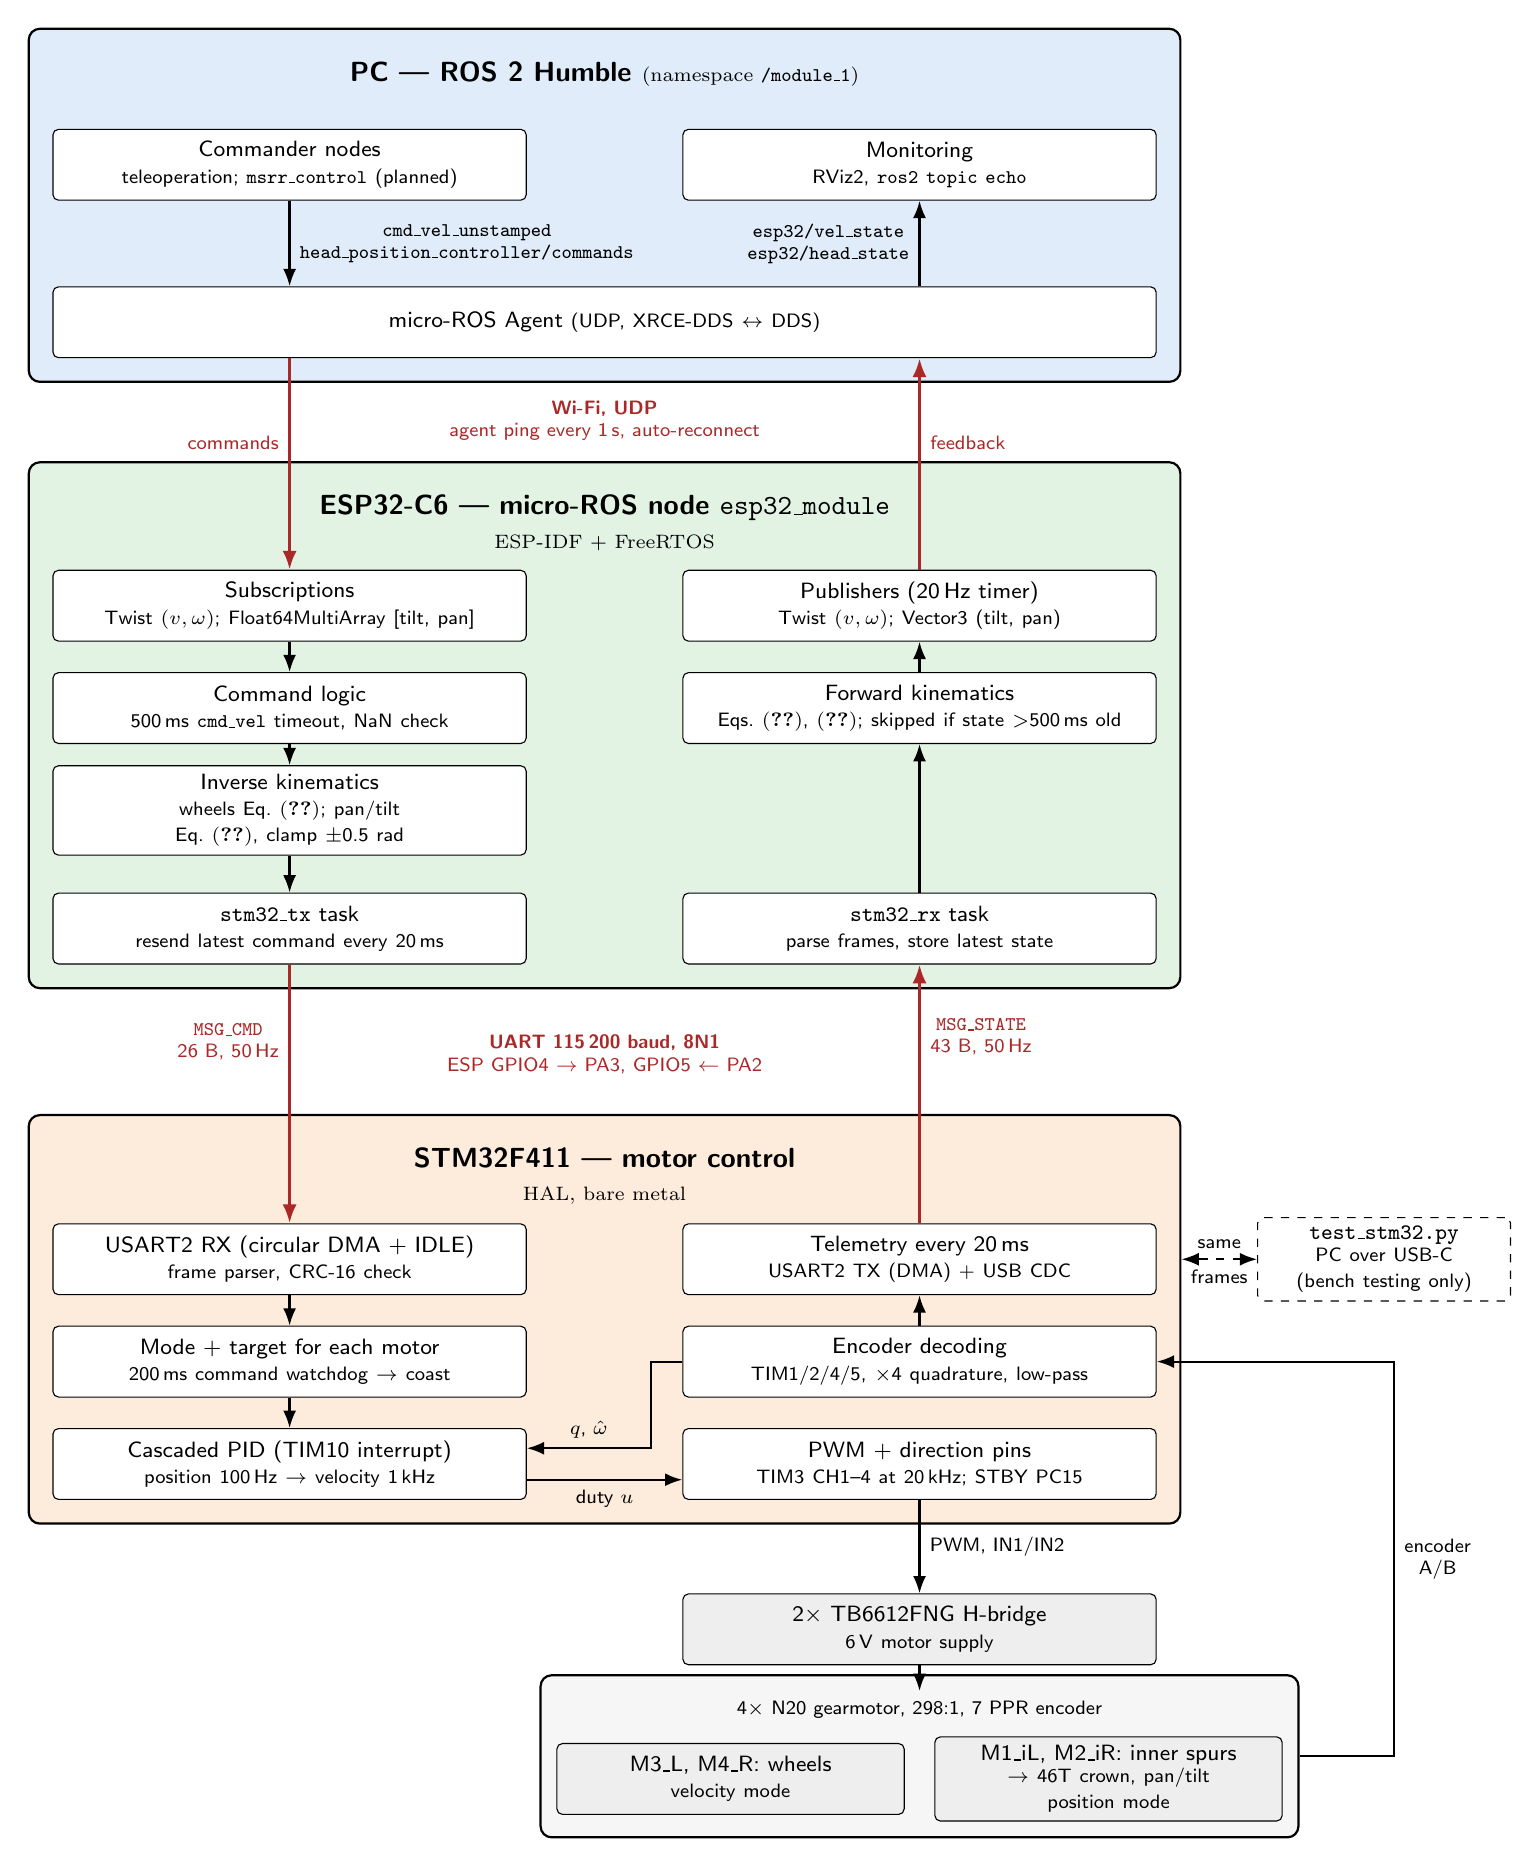
\begin{tikzpicture}[
  font=\sffamily\footnotesize,
  blk/.style={draw, rounded corners=2pt, fill=white, align=center, text width=58mm, minimum height=9mm, inner sep=3pt},
  grp/.style={draw, rounded corners=4pt, inner sep=3mm, thick},
  ttl/.style={font=\sffamily\bfseries, align=center},
  arr/.style={-{Latex[length=2.2mm]}, thick},
  red/.style={-{Latex[length=2.4mm]}, very thick, linkred},
  note/.style={font=\sffamily\scriptsize, align=center},
]
% ---------------- PC ----------------
\node[ttl] (pct) at (4,1.15) {PC --- ROS 2 Humble \normalfont\scriptsize(namespace \texttt{/module\_1})};
\node[blk] (cmdr) at (0,0) {Commander nodes\\ \scriptsize teleoperation; \texttt{msrr\_control} (planned)};
\node[blk] (mon)  at (8,0) {Monitoring\\ \scriptsize RViz2, \texttt{ros2 topic echo}};
\node[blk, text width=138mm] (agent) at (4,-2.0) {micro-ROS Agent \scriptsize(UDP, XRCE-DDS $\leftrightarrow$ DDS)};
\draw[arr] (cmdr.south) -- node[note, right] {\texttt{cmd\_vel\_unstamped}\\\texttt{head\_position\_controller/commands}} (cmdr.south |- agent.north);
\draw[arr] (mon.south |- agent.north) -- node[note, left] {\texttt{esp32/vel\_state}\\\texttt{esp32/head\_state}} (mon.south);
\begin{scope}[on background layer]
\node[grp, fill=pcblue, fit=(pct)(cmdr)(mon)(agent)] (pc) {};
\end{scope}

% ---------------- ESP32 ----------------
\node[ttl] (espt) at (4,-4.55) {ESP32-C6 --- micro-ROS node \texttt{esp32\_module}\\ \normalfont\scriptsize ESP-IDF + FreeRTOS};
\node[blk] (subs)  at (0,-5.6)  {Subscriptions\\ \scriptsize Twist $(v,\omega)$; Float64MultiArray [tilt, pan]};
\node[blk] (logic) at (0,-6.9)  {Command logic\\ \scriptsize 500\,ms \texttt{cmd\_vel} timeout, NaN check};
\node[blk] (ik)    at (0,-8.2)  {Inverse kinematics\\ \scriptsize wheels Eq.~\eqref{pr3:eq:ik}; pan/tilt Eq.~\eqref{pr3:eq:ptik}, clamp $\pm$0.5 rad};
\node[blk] (tx)    at (0,-9.7)  {\texttt{stm32\_tx} task\\ \scriptsize resend latest command every 20\,ms};
\node[blk] (pubs)  at (8,-5.6)  {Publishers (20\,Hz timer)\\ \scriptsize Twist $(v,\omega)$; Vector3 (tilt, pan)};
\node[blk] (fk)    at (8,-6.9)  {Forward kinematics\\ \scriptsize Eqs.~\eqref{pr3:eq:fk}, \eqref{pr3:eq:ptfk}; skipped if state $>$500\,ms old};
\node[blk] (rx)    at (8,-9.7)  {\texttt{stm32\_rx} task\\ \scriptsize parse frames, store latest state};
\draw[arr] (subs) -- (logic);
\draw[arr] (logic) -- (ik);
\draw[arr] (ik) -- (tx);
\draw[arr] (rx) -- (fk);
\draw[arr] (fk) -- (pubs);
\begin{scope}[on background layer]
\node[grp, fill=espgreen, fit=(espt)(subs)(tx)(pubs)(rx)] (esp) {};
\end{scope}

% PC <-> ESP link
\draw[red] (cmdr.south |- agent.south) -- node[note, left, text=linkred, pos=0.4] {commands} (subs.north);
\draw[red] (pubs.north) -- node[note, right, text=linkred, pos=0.6] {feedback} (mon.south |- agent.south);
\node[note, text=linkred] at (4,-3.25) {\textbf{Wi-Fi, UDP}\\ agent ping every 1\,s, auto-reconnect};

% ---------------- STM32 ----------------
\node[ttl] (stmt) at (4,-12.85) {STM32F411 --- motor control\\ \normalfont\scriptsize HAL, bare metal};
\node[blk] (parse) at (0,-13.90) {USART2 RX (circular DMA + IDLE)\\ \scriptsize frame parser, CRC-16 check};
\node[blk] (wd)    at (0,-15.20) {Mode + target for each motor\\ \scriptsize 200\,ms command watchdog $\rightarrow$ coast};
\node[blk] (pid)   at (0,-16.50) {Cascaded PID (TIM10 interrupt)\\ \scriptsize position 100\,Hz $\rightarrow$ velocity 1\,kHz};
\node[blk] (tele)  at (8,-13.90) {Telemetry every 20\,ms\\ \scriptsize USART2 TX (DMA) + USB CDC};
\node[blk] (enc)   at (8,-15.20) {Encoder decoding\\ \scriptsize TIM1/2/4/5, $\times$4 quadrature, low-pass};
\node[blk] (pwm)   at (8,-16.50) {PWM + direction pins\\ \scriptsize TIM3 CH1--4 at 20\,kHz; STBY PC15};
\draw[arr] (parse) -- (wd);
\draw[arr] (wd) -- (pid);
\draw[arr] ([yshift=-2mm]pid.east) -- node[note, below] {duty $u$} ([yshift=-2mm]pwm.west);
\draw[arr] (enc.west) -- ++(-0.4,0) |- node[note, pos=0.75, above] {$q$, $\hat\omega$} ([yshift=2mm]pid.east);
\draw[arr] (enc) -- (tele);
\begin{scope}[on background layer]
\node[grp, fill=stmorange, fit=(stmt)(parse)(pid)(tele)(pwm)] (stm) {};
\end{scope}

% ESP <-> STM link
\draw[red] (tx.south) -- node[note, left, text=linkred, pos=0.3] {\texttt{MSG\_CMD}\\26 B, 50\,Hz} (parse.north);
\draw[red] (tele.north) -- node[note, right, text=linkred, pos=0.72] {\texttt{MSG\_STATE}\\43 B, 50\,Hz} (rx.south);
\node[note, text=linkred] at (4,-11.3) {\textbf{UART 115\,200 baud, 8N1}\\ ESP GPIO4 $\rightarrow$ PA3, GPIO5 $\leftarrow$ PA2};

% USB bench tool
\node[blk, dashed, text width=30mm] (usb) at (13.9,-13.90) {\texttt{test\_stm32.py}\\ \scriptsize PC over USB-C\\(bench testing only)};
\draw[dashed, thick, {Latex[length=2.2mm]}-{Latex[length=2.2mm]}] (usb.west) -- node[note, above] {same} node[note, below] {frames} (stm.east |- usb.west);

% ---------------- Hardware ----------------
\node[blk, fill=hwgray] (tb) at (8,-18.60) {2$\times$ TB6612FNG H-bridge\\ \scriptsize 6\,V motor supply};
\node[blk, fill=hwgray, text width=42mm] (wheels) at (5.6,-20.50) {M3\_L, M4\_R: wheels\\ \scriptsize velocity mode};
\node[blk, fill=hwgray, text width=42mm] (inner)  at (10.4,-20.50) {M1\_iL, M2\_iR: inner spurs\\ \scriptsize $\rightarrow$ 46T crown, pan/tilt\\ \scriptsize position mode};
\node[font=\sffamily\scriptsize, anchor=south] (motl) at (8,-19.85) {4$\times$ N20 gearmotor, 298:1, 7 PPR encoder};
\begin{scope}[on background layer]
\node[grp, fill=hwgray!50, fit=(wheels)(inner)(motl), inner sep=2mm] (mot) {};
\end{scope}
\draw[arr] (pwm) -- node[note, right] {PWM, IN1/IN2} (tb);
\draw[arr] (tb) -- (motl.north);
\draw[arr] (mot.east) -- ++(1.2,0) |- node[note, pos=0.25, right] {encoder\\A/B} (enc.east);
\end{tikzpicture}}
\caption{Teleoperation and embedded system architecture (replaces the architecture figure of Progress Report~2). The PC sends
body-level commands through micro-ROS; each module's ESP32-C6 computes the joint targets and
the STM32F411 closes the motor loops. Red arrows are the two communication links. The dashed
USB path is used only for bench testing without the ESP32.}
\label{fig:teleop-architecture}
\end{figure}

\paragraph{Why micro-ROS.} PR2 planned a custom \texttt{ros2\_control} hardware plugin on the
PC that packed wheel targets into UDP packets, with the ESP32 only forwarding bytes to the
STM32. With micro-ROS the ESP32-C6 becomes a normal ROS~2 node instead:
\begin{itemize}
  \item No custom PC plugin or custom UDP packet format has to be written and maintained.
        The module's topics appear in the ROS graph and can be inspected with standard tools
        (\texttt{ros2 topic list}, \texttt{ros2 topic echo}), which makes debugging easier.
  \item The command topics have the \emph{same names and message types} as the controllers in
        the Gazebo simulation (Section~\ref{sec:sim-model}). A commander node can therefore drive the simulated or the real
        module without changes (tested so far with teleoperation only).
  \item Kinematics run on each module, and the PC sends only body-level commands. This fits
        the distributed SMORES-EP design and scales to $N$ modules, one namespace each
        (\texttt{/module\_1}, \texttt{/module\_2}, \dots). It is also a step towards the onboard
        computation of Phase~D.
  \item The micro-ROS session is checked with a ping every second and is re-created
        automatically when the connection returns (Section~\ref{pr3:sec:agent}).
\end{itemize}
Two trade-offs were accepted. The module namespace and the agent IP address are build-time
settings, so each module currently needs its own build. On hardware the module publishes its
measured velocity on \texttt{esp32/vel\_state} instead of \texttt{ros2\_control} producing
\texttt{/odom} and \texttt{/joint\_states}.

% ----------------------------------------------------------------------
\subsection{ROS 2 Interface}
% ----------------------------------------------------------------------

Table~\ref{pr3:tab:topics} lists the module's ROS~2 interface. All names are relative to the
module namespace (\texttt{/module\_1} for the first module).

\begin{table}[H]
\centering
\caption{ROS~2 topics of the micro-ROS node \texttt{esp32\_module}.}
\label{pr3:tab:topics}
\small
\begin{tabularx}{\linewidth}{l c >{\raggedright\arraybackslash}X}
\toprule
Topic and message type & Dir. & Content \\
\midrule
\texttt{diff\_drive\_controller/cmd\_vel\_unstamped} & sub & \texttt{linear.x} $=v$ [m/s], \texttt{angular.z} $=\omega$ [rad/s] \\
\quad\footnotesize\texttt{geometry\_msgs/Twist} & & \\[2pt]
\texttt{head\_position\_controller/commands} & sub & \texttt{data} $=[\theta_\text{tilt},\theta_\text{pan}]$ [rad] \\
\quad\footnotesize\texttt{std\_msgs/Float64MultiArray} & & \\[2pt]
\texttt{esp32/vel\_state} & pub & measured $v$, $\omega$ from the wheel encoders, 20\,Hz \\
\quad\footnotesize\texttt{geometry\_msgs/Twist} & & \\[2pt]
\texttt{esp32/head\_state} & pub & \texttt{x} $=\theta_\text{tilt}$, \texttt{y} $=\theta_\text{pan}$ [rad], 20\,Hz \\
\quad\footnotesize\texttt{geometry\_msgs/Vector3} & & \\
\bottomrule
\end{tabularx}
\end{table}

% ----------------------------------------------------------------------
\subsection{ESP32-C6 Firmware}
\label{pr3:sec:esp}
% ----------------------------------------------------------------------

The firmware (ESP-IDF project \texttt{smores\_esp32c6}) uses the micro-ROS component for
ESP-IDF on the Humble branch (\texttt{micro\_ros\_espidf\_component} \texttt{\^{}22}) with the
default XRCE-DDS middleware over Wi-Fi. The Wi-Fi network and the agent's IP address and
port are set in \texttt{menuconfig}. It is split into the files in Table~\ref{pr3:tab:espfiles}
and runs the FreeRTOS tasks in Table~\ref{pr3:tab:esptasks}.

\begin{table}[H]
\centering
\caption{ESP32-C6 source files.}
\label{pr3:tab:espfiles}
\small
\begin{tabularx}{\linewidth}{l >{\raggedright\arraybackslash}X}
\toprule
File & Purpose \\
\midrule
\texttt{robot\_config.h} & All per-module settings: namespace, topic names, UART pins, timing, wheel radius and separation, pan/tilt gains and limits \\
\texttt{main.c} & micro-ROS entities, subscription callbacks, 20\,Hz feedback timer, agent connection state machine \\
\texttt{robot\_logic.c} & Stores the latest commands and builds the 4-motor STM32 command (mode + target), including the \texttt{cmd\_vel} timeout \\
\texttt{kinematics.c} & Differential-drive and pan/tilt inverse and forward kinematics \\
\texttt{stm32\_link.c} & UART driver and the RX/TX tasks; shares the latest command and state under a spinlock \\
\texttt{protocol.c} & Frame builder and byte-by-byte parser with CRC-16 (same file as on the STM32) \\
\bottomrule
\end{tabularx}
\end{table}

\begin{table}[H]
\centering
\caption{FreeRTOS tasks on the ESP32-C6 (micro-ROS task values are the project defaults in \texttt{Kconfig.projbuild}).}
\label{pr3:tab:esptasks}
\small
\begin{tabularx}{\linewidth}{l c c >{\raggedright\arraybackslash}X}
\toprule
Task & Priority & Stack & Work \\
\midrule
\texttt{uros\_task}  & 5 & \SI{16000}{B} & micro-ROS executor (2 subscriptions + 1 timer), agent ping and reconnection \\
\texttt{stm32\_tx}   & 6 & \SI{3072}{B}  & Sends the latest \texttt{MSG\_CMD} every \SI{20}{ms} (\texttt{vTaskDelayUntil}) \\
\texttt{stm32\_rx}   & 6 & \SI{3072}{B}  & Reads the UART, parses frames, stores the latest \texttt{MSG\_STATE}; 1\,Hz debug log \\
\bottomrule
\end{tabularx}
\end{table}

The callbacks only store the new command and rebuild the STM32 command; the
\texttt{stm32\_tx} task sends it. Sending at a fixed \SI{50}{Hz}, independent of how often
ROS publishes, keeps the STM32 watchdog (\SI{200}{ms}) fed while the PC is connected.

\subsubsection{Wheel Kinematics}

With wheel radius $r=\SI{50}{mm}$ and wheel separation $L=\SI{99.9}{mm}$, the inverse
kinematics give the wheel angular velocities from the body command $(v,\omega)$:
\begin{equation}
  \omega_L = \frac{v-\omega L/2}{r}, \qquad \omega_R = \frac{v+\omega L/2}{r}.
  \label{pr3:eq:ik}
\end{equation}
The installed wheels turn opposite to the ROS convention, so both targets are multiplied
by a sign $s_\text{drive}=-1$ before they are sent; the encoder signs are not changed.
The measured wheel velocities are converted back with the forward kinematics:
\begin{equation}
  v = \frac{r}{2}\,(\omega_R+\omega_L), \qquad \omega = \frac{r}{L}\,(\omega_R-\omega_L).
  \label{pr3:eq:fk}
\end{equation}
As a check, the top speed in Section~\ref{sec:sim-model} ($v=\SI{0.049}{m/s}$) gives
$\omega_L=\omega_R=\SI{0.98}{rad/s}$ at the wheel. This equals the free speed of the
48T spur gear (\SI{50}{rpm} N20 output $\times\,9/48 = \SI{9.4}{rpm}$).

\subsubsection{Pan/Tilt Kinematics}

The pan/tilt mixing equation in Section~\ref{sec:sim-model} left the mixing to the firmware; it is now implemented on the ESP32.
Let $q_\text{iL}$ and $q_\text{iR}$ be the angles of the two inner 48T spur gears. Turning
both the same way tilts the face; turning them in opposite directions spins the 46T crown
gear (pan):
\begin{equation}
  q_\text{iL} = \frac{\theta_\text{tilt}}{K_t} + \frac{\theta_\text{pan}}{K_p}, \qquad
  q_\text{iR} = \frac{\theta_\text{tilt}}{K_t} - \frac{\theta_\text{pan}}{K_p},
  \label{pr3:eq:ptik}
\end{equation}
\begin{equation}
  \theta_\text{tilt} = K_t\,\frac{q_\text{iL}+q_\text{iR}}{2}, \qquad
  \theta_\text{pan}  = K_p\,\frac{q_\text{iL}-q_\text{iR}}{2},
  \label{pr3:eq:ptfk}
\end{equation}
with $K_t=1$ and $K_p=48/46$, the same relation as in the simulation's
\texttt{ros2\_control} xacro. In the notation of that equation this is $N_t=1$ and
$N_p=46/48$ at the spur-gear level; the remaining motor-to-spur reduction
($298\times48/9$) is handled by the encoder scaling on the STM32 (Eq.~\eqref{pr3:eq:cpr}).
Before Eq.~\eqref{pr3:eq:ptik} is applied, $\theta_\text{pan}$ and $\theta_\text{tilt}$ are
clamped to $\pm\SI{0.5}{rad}$, a conservative range for first tests.

\subsubsection{Agent Connection Handling}
\label{pr3:sec:agent}

The micro-ROS task follows the reconnection pattern of Figure~\ref{pr3:fig:agent}. ROS entities
(node, subscriptions, publishers, timer, executor) exist only while the agent answers.
When the agent is lost they are destroyed without waiting for the agent, and the task
goes back to waiting. While it waits, the task keeps applying the \texttt{cmd\_vel} timeout,
so the wheels are commanded to \SI{0}{rad/s} instead of repeating the last command.

\begin{figure}[H]
\centering
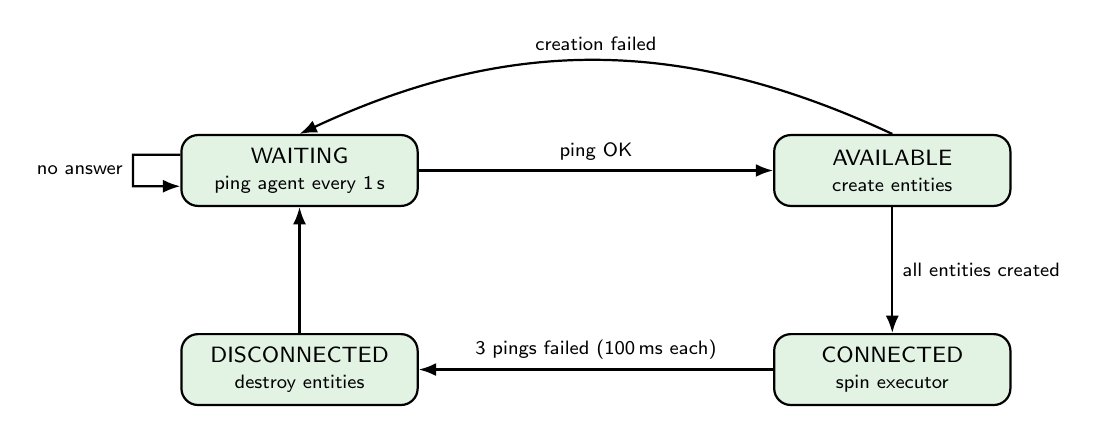
\begin{tikzpicture}[
  font=\sffamily\footnotesize, node distance=16mm and 45mm,
  st/.style={draw, rounded corners=6pt, thick, minimum width=30mm, minimum height=9mm, align=center, fill=espgreen},
  arr/.style={-{Latex[length=2.2mm]}, thick},
  tl/.style={font=\sffamily\scriptsize, align=center}
]
\node[st] (w) {WAITING\\ \scriptsize ping agent every 1\,s};
\node[st, right=of w] (a) {AVAILABLE\\ \scriptsize create entities};
\node[st, below=of a] (c) {CONNECTED\\ \scriptsize spin executor};
\node[st, below=of w] (d) {DISCONNECTED\\ \scriptsize destroy entities};
\draw[arr] (w) -- node[tl, above] {ping OK} (a);
\draw[arr] (a) -- node[tl, right] {all entities created} (c);
\draw[arr] (a.north) to[bend right=25] node[tl, above] {creation failed} (w.north);
\draw[arr] (c) -- node[tl, above] {3 pings failed (100\,ms each)} (d);
\draw[arr] (d) -- node[tl, left] {} (w);
\draw[arr] ([yshift=2mm]w.west) -- ++(-6mm,0) -- ++(0,-4mm) node[tl, left, pos=0.5] {no answer} -- ([yshift=-2mm]w.west);
\end{tikzpicture}
\caption{micro-ROS agent connection state machine on the ESP32-C6.}
\label{pr3:fig:agent}
\end{figure}

% ----------------------------------------------------------------------
\subsection{ESP32--STM32 Link Protocol}
% ----------------------------------------------------------------------

The ESP32-C6 (UART1, TX GPIO4, RX GPIO5) and the STM32 (USART2, PA3/PA2) exchange binary
frames at \SI{115200}{baud}, 8N1. The same frame format is used on the STM32's USB-C virtual
COM port, so the STM32 can also be driven from the PC without the ESP32. One source file,
\texttt{protocol.c}, is shared by both microcontrollers.

\begin{table}[H]
\centering
\caption{Frame format (multi-byte values little-endian, floats IEEE-754 single precision).}
\label{pr3:tab:frame}
\small
\begin{tabular}{ccccccc}
\toprule
\texttt{0xAA} & \texttt{0x55} & TYPE & LEN & PAYLOAD & CRC\_lo & CRC\_hi \\
\midrule
1 B & 1 B & 1 B & 1 B & 0--48 B & 1 B & 1 B \\
\bottomrule
\end{tabular}

\vspace{2mm}
\parbox{0.92\linewidth}{\footnotesize CRC-16/CCITT-FALSE (polynomial \texttt{0x1021}, initial value
\texttt{0xFFFF}) over TYPE, LEN and PAYLOAD. The parser is a byte-by-byte state machine: it
resynchronises on the two start bytes, rejects lengths above 48 bytes, and silently drops
frames with a wrong CRC.}
\end{table}

\begin{table}[H]
\centering
\caption{Message types. Motor index order everywhere: [0] M1\_iL, [1] M2\_iR, [2] M3\_L, [3] M4\_R.}
\label{pr3:tab:msgs}
\small
\begin{tabularx}{\linewidth}{l l c >{\raggedright\arraybackslash}X}
\toprule
Message & Direction & Payload & Content \\
\midrule
\texttt{MSG\_CMD} (\texttt{0x01})   & ESP32 $\rightarrow$ STM32 & 20 B & \texttt{uint8 mode[4]}, \texttt{float target[4]}. Modes: 0 = stop (coast), 1 = velocity [rad/s], 2 = position [rad], 3 = duty [$-1$..1, open loop] \\
\texttt{MSG\_ZERO} (\texttt{0x04})  & ESP32 $\rightarrow$ STM32 & 1 B  & Bit mask: set the position of the selected motors to zero \\
\texttt{MSG\_STATE} (\texttt{0x81}) & STM32 $\rightarrow$ ESP32 & 37 B & \texttt{uint32 stamp\_ms}, \texttt{float pos[4]} [rad], \texttt{float vel[4]} [rad/s], \texttt{uint8 flags} (bit 0 = watchdog tripped) \\
\bottomrule
\end{tabularx}
\end{table}

At \SI{115200}{baud} with 10 bits per byte the link carries \SI{11520}{B/s} in each direction.
A command frame is 26 bytes (\SI{2.3}{ms} on the wire) and a state frame is 43 bytes
(\SI{3.7}{ms}). At \SI{50}{Hz} they use about 11\,\% and 19\,\% of the two directions,
which leaves margin for more messages in Phase~B (for example EP-Face commands).

% ----------------------------------------------------------------------
\subsection{STM32F411 Firmware}
\label{pr3:sec:stm}
% ----------------------------------------------------------------------

The CubeMX configuration of Section~\ref{sec:phase-a1-hw} is kept: \SI{96}{MHz} system clock,
TIM3 PWM at \SI{20}{kHz}, four timers in $\times4$ encoder mode, TIM10 interrupt at
\SI{1}{kHz}, USART2 with DMA, and USB CDC. The project is built with CMake and
\texttt{arm-none-eabi-gcc} in VS Code. The application code is in five files:
\texttt{config.h} (all tunable numbers), \texttt{motor.c} (PWM, direction and encoder
access), \texttt{pid.c}, \texttt{protocol.c} and \texttt{app.c} (control loop, frame handling,
telemetry, watchdog). CubeMX-generated \texttt{main.c} only calls \texttt{App\_Init()} and
\texttt{App\_MainLoop()}.

\subsubsection{Motor Channel Assignment}

During bring-up the motors were renumbered by their physical role, and the direction and
encoder signs were calibrated so that a positive duty gives a positive encoder count on
every channel. The pin labels
in the CubeMX \texttt{.ioc} file still carry the old names. The direction pins of M2\_iR and M3\_L moved when the UWB socket was added on the A-1 carrier board (Section~\ref{sec:phase-a1-hw}).

\begin{table}[H]
\centering
\caption{Motor channel assignment and calibrated signs.}
\label{pr3:tab:pins}
\footnotesize
\begin{tabular}{c l l l l l c c}
\toprule
Idx & Name & Role & PWM & IN1 / IN2 & Encoder & Dir. & Enc. \\
\midrule
0 & M1\_iL & inner left  & CH3, PB0 & PA4 / PA5   & TIM4 (PB6, PB7), 16-bit  & $-1$ & $+1$ \\
1 & M2\_iR & inner right & CH2, PA7 & PB8 / PB9 & TIM2 (PA15, PB3), 32-bit & $+1$ & $-1$ \\
2 & M3\_L  & left wheel       & CH1, PA6 & PB12 / PA10 & TIM1 (PA8, PA9), 16-bit  & $-1$ & $+1$ \\
3 & M4\_R  & right wheel      & CH4, PB1 & PB4 / PB5   & TIM5 (PA0, PA1), 32-bit  & $+1$ & $-1$ \\
\midrule
\multicolumn{8}{l}{PWM from TIM3. Driver standby (both TB6612FNG): \textbf{PC15} (PR2 listed PB10). LED: PC13.} \\
\bottomrule
\end{tabular}
\end{table}

\subsubsection{Encoder Scaling and Velocity Estimate}

Every motor is reported as the angle of its 48T spur gear. With the 7~PPR encoder on the
motor shaft, $\times4$ decoding, the 298:1 N20 gearbox and the 9T/48T stage, one spur-gear
revolution is
\begin{equation}
  N_c = 4 \cdot 7 \cdot 298 \cdot \frac{48}{9} = \num{44501}\ \text{counts},
  \qquad \Delta\theta = \frac{2\pi}{N_c} = \SI{1.41e-4}{rad}\ (\ang{0.0081}).
  \label{pr3:eq:cpr}
\end{equation}
This resolution is much finer than the \SI{0.2}{mm} gear backlash allowance (about
\SI{0.27}{\degree} at the 48T spur gear, or about 33 counts), so the encoder measures motor
motion rather than the true output angle.

The velocity is computed every $T=\SI{1}{ms}$ from the count change $\Delta n_k$ and smoothed
with a first-order low-pass filter:
\begin{equation}
  \hat\omega_k = \hat\omega_{k-1} + \alpha\left(\frac{2\pi}{N_c}\frac{\Delta n_k}{T}-\hat\omega_{k-1}\right),
  \qquad \alpha = 0.1 .
\end{equation}
One count in one tick is $2\pi/(N_c T)=\SI{0.14}{rad/s}$, about 14\,\% of the top speed, so the
raw estimate is coarse. The filter ($\tau\approx\SI{9.5}{ms}$) smooths it. The 16-bit
timers are unwrapped through a signed 16-bit difference and the 32-bit timers through a
signed 32-bit difference, so counter overflow does not cause jumps.

\subsubsection{Control Loop}

The \SI{1}{kHz} TIM10 interrupt runs the controller in Figure~\ref{pr3:fig:pid} for each motor.
In velocity mode the target is the velocity reference $\omega^*$ directly. In position mode
an outer P loop, run every tenth tick (\SI{100}{Hz}), turns the position error into
$\omega^*$, limited to $\pm\SI{0.9}{rad/s}$ (just below the \SI{0.98}{rad/s} top speed).
The inner loop is a PI controller with velocity feed-forward:
\begin{equation}
  u = \operatorname{sat}_{\pm d_\text{max}}\!\Big(K_\text{ff}\,\omega^* + K_p e + K_i\!\int e\,dt + K_d\,\tfrac{d}{dt}(-\hat\omega)\Big),
  \qquad e = \omega^*-\hat\omega .
\end{equation}
The derivative acts on the measurement, so a step in the setpoint gives no derivative kick.
The integrator uses conditional integration (anti-windup): it is only updated when the output
is not saturated or when the error drives the output back out of saturation. The PID output
limit is set equal to the duty limit $d_\text{max}$ in \texttt{Motor\_SetDuty()}, so the
integrator cannot wind up against a limit it does not know about. When a motor's mode
changes, its PID states are reset. Duty mode bypasses the controller (used for testing),
and stop mode coasts the motor (IN1 = IN2 = low).

\begin{figure}[H]
\centering
\resizebox{\linewidth}{!}{%
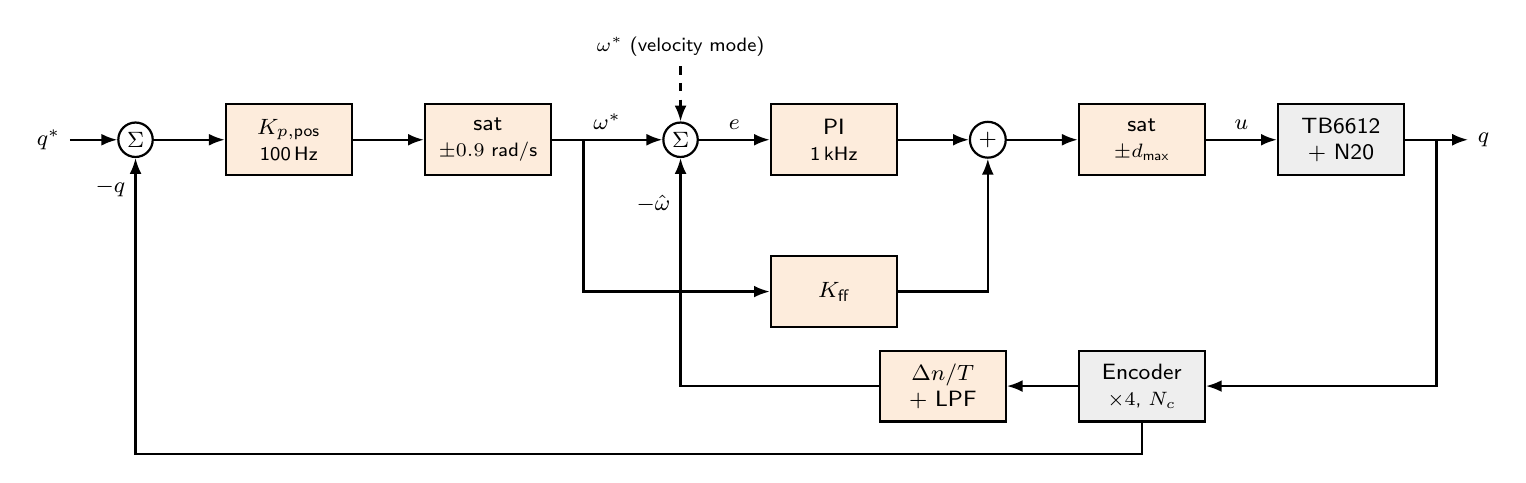
\begin{tikzpicture}[
  font=\sffamily\footnotesize, node distance=9mm,
  b/.style={draw, thick, minimum height=9mm, minimum width=16mm, align=center, fill=stmorange},
  s/.style={draw, thick, circle, inner sep=1.5pt},
  arr/.style={-{Latex[length=2mm]}, thick}
]
\node (in) {$q^*$};
\node[s, right=6mm of in] (s1) {$\Sigma$};
\node[b, right=of s1] (kp) {$K_{p,\text{pos}}$\\ \scriptsize 100\,Hz};
\node[b, right=of kp] (sat1) {sat\\ \scriptsize $\pm0.9$ rad/s};
\node[s, right=14mm of sat1] (s2) {$\Sigma$};
\node[b, right=of s2] (pi) {PI\\ \scriptsize 1\,kHz};
\node[s, right=of pi] (s3) {$+$};
\node[b, right=of s3] (sat2) {sat\\ \scriptsize $\pm d_\text{max}$};
\node[b, right=of sat2, fill=hwgray] (plant) {TB6612\\+ N20};
\node[right=8mm of plant] (out) {$q$};
\node[b, below=10mm of pi] (ff) {$K_\text{ff}$};
\node[b, below=22mm of sat2, fill=hwgray] (enc) {Encoder\\ \scriptsize $\times4$, $N_c$};
\node[b, left=of enc] (lpf) {$\Delta n/T$\\ + LPF};
\node[above=7mm of s2] (vin) {\scriptsize $\omega^*$ (velocity mode)};
\draw[arr] (in) -- (s1);
\draw[arr] (s1) -- (kp);
\draw[arr] (kp) -- (sat1);
\draw[arr] (sat1) -- node[above] {$\omega^*$} (s2);
\draw[arr, dashed] (vin) -- (s2);
\draw[arr] (s2) -- node[above] {$e$} (pi);
\draw[arr] (pi) -- (s3);
\draw[arr] (s3) -- (sat2);
\draw[arr] (sat2) -- node[above] {$u$} (plant);
\draw[arr] (plant) -- (out);
\draw[arr] ($(sat1.east)+(4mm,0)$) |- (ff);
\draw[arr] (ff) -| (s3);
\draw[arr] ($(plant.east)+(4mm,0)$) |- (enc);
\draw[arr] (enc) -- (lpf);
\draw[arr] (lpf) -| node[pos=0.9, left] {$-\hat\omega$} (s2);
\draw[arr] (enc.south) -- ++(0,-4mm) -| node[pos=0.95, left] {$-q$} (s1);
\end{tikzpicture}}
\caption{Cascaded controller run for each motor on the STM32. Wheels use velocity mode (the
dashed input); the inner pan/tilt gears use position mode.}
\label{pr3:fig:pid}
\end{figure}

\begin{table}[H]
\centering
\caption{Controller parameters (starting values, still to be tuned on the module).}
\label{pr3:tab:gains}
\small
\begin{tabular}{l c p{6.2cm}}
\toprule
Parameter & Value & Note \\
\midrule
$K_p$, $K_i$, $K_d$ (velocity) & 0.30, 1.50, 0 & duty per rad/s \\
$K_\text{ff}$ & 0.80 & slightly below $1/0.98$ so a stronger motor does not overshoot \\
$K_{p,\text{pos}}$, $K_{i,\text{pos}}$, $K_{d,\text{pos}}$ & 0.80, 0, 0 & kept low because the velocity signal is coarse \\
Position-loop velocity limit & \SI{0.9}{rad/s} & \\
Duty limit $d_\text{max}$ & 1.0 & full duty allowed \\
Velocity filter $\alpha$ & 0.10 & \\
\bottomrule
\end{tabular}
\end{table}

The starting gains were chosen by simulating the firmware's control code against a DC-motor
model built from the rated motor data (\SI{6}{V}, about \SI{0.98}{rad/s} at the spur gear at
full duty). They were checked on several variations of that model (faster, slower, weaker,
stronger, with a dead zone). They are a safe starting point, not final values.

\subsubsection{Interrupts and Data Flow}

The control tick (TIM10) has NVIC priority 1, and the USART2 and DMA interrupts have
priority 2, so the control loop always pre-empts frame parsing. USART2 receives into a
256-byte circular DMA buffer; the receive-to-idle callback passes only the new bytes to the
parser, including when the buffer wraps around. When a valid command arrives, the parser
copies all four modes and targets inside a short critical section, so the control loop never
uses a half-updated command. Targets that are NaN or infinite, and unknown modes, are replaced
by stop. Telemetry is sent from the main loop every \SI{20}{ms} with non-blocking DMA, on
USART2 and, when a PC is connected, on USB CDC. A UART error restarts reception from the main
loop. The LED shows the link state: a \SI{500}{ms} blink when commands arrive, \SI{250}{ms}
when the watchdog has tripped.

% ----------------------------------------------------------------------
\subsection{Safety and Fault Handling}
% ----------------------------------------------------------------------

\begin{table}[H]
\centering
\caption{Fault handling at each level.}
\label{pr3:tab:safety}
\small
\begin{tabularx}{\linewidth}{l l >{\raggedright\arraybackslash}X}
\toprule
Fault & Detected by & Reaction \\
\midrule
PC stops publishing \texttt{cmd\_vel}       & ESP32, 500\,ms timeout & Wheels commanded to \SI{0}{rad/s} (held, not coasting) \\
micro-ROS agent lost                      & ESP32, 3 failed pings  & Entities destroyed, reconnect loop; wheel timeout still applied \\
ESP32 stops sending (crash, cable)        & STM32, 200\,ms watchdog & All motors coast; flag in \texttt{MSG\_STATE}; fast LED blink \\
Corrupted or partial frame                & CRC-16, length check   & Frame dropped \\
NaN/Inf or unknown mode in a command      & ESP32 and STM32        & Command ignored (ESP32) or motor set to stop (STM32) \\
Pan/tilt command out of range             & ESP32 IK               & Clamped to $\pm\SI{0.5}{rad}$ \\
Stale feedback from the STM32 ($>$500\,ms)& ESP32                  & Feedback topics not published \\
Power-up, before any command              & both                   & All motors in stop; TB6612 kept in standby until the STM32 is set up \\
\bottomrule
\end{tabularx}
\end{table}

% ----------------------------------------------------------------------
\subsection{Bring-up and Test Results}
\label{pr3:sec:test}
% ----------------------------------------------------------------------

The system was brought up one level at a time, so each fault could be traced to one part:

\begin{enumerate}
  \item \textbf{STM32 alone, over USB-C.} The Python tool \texttt{test\_stm32.py} sends the same
        frames as the ESP32 over the USB virtual COM port. Its modes (\texttt{monitor},
        \texttt{duty}, \texttt{vel}, \texttt{pos}, \texttt{zero}) were used to run each motor, read all
        four encoders, and calibrate the direction and encoder signs in Table~\ref{pr3:tab:pins}.
        All four motors run under the STM32 firmware.
  \item \textbf{ESP32 $\rightarrow$ STM32 link.} A test build of the ESP32 firmware runs one
        motor at a time at 30\,\% duty for \SI{2}{s}, with a \SI{2}{s} stop in between. This
        confirmed the UART wiring and that index $i$ on the ESP32 moves the same physical motor
        as index $i$ on the STM32, which led to the renumbering in Table~\ref{pr3:tab:pins}.
  \item \textbf{Full chain through micro-ROS.} With the micro-ROS agent running on the PC,
        velocity commands (\texttt{Twist}) from a teleoperation node, sent on the module's
        wheel-command topic (Table~\ref{pr3:tab:topics}), drive the module. The wheel
        kinematics and the wheel direction sign work on the real module. Only the wheels were tested in this step; no
        pan/tilt commands were sent.
\end{enumerate}

\noindent\textbf{Result:} the wheel locomotion of the SMORES-EP style module works with the
architecture of Figure~\ref{fig:teleop-architecture}. The pan/tilt path (Eqs.~\eqref{pr3:eq:ptik}--\eqref{pr3:eq:ptfk},
position mode) is implemented in both firmwares but has \emph{not yet been tested} on the
module through ROS~2.

\subsubsection{Teleoperation Video}

A video of the module being teleoperated from the PC is available on Google Drive. Velocity
commands sent from ROS~2 drive the wheels through micro-ROS
(Figure~\ref{pr3:fig:video}).

\begin{figure}[H]
\centering
\begin{tabular}{c p{0.62\linewidth}}
\raisebox{-0.5\height}{\href{https://drive.google.com/file/d/1tHmvNSHuG8BPgNlsanB781ZCGBjsgjm0/view?usp=sharing}{\qrcode[nolink,height=2.8cm]{https://drive.google.com/file/d/1tHmvNSHuG8BPgNlsanB781ZCGBjsgjm0/view?usp=sharing}}} &
\raggedright Scan the QR code or open:\\[1mm]
\footnotesize\url{https://drive.google.com/file/d/1tHmvNSHuG8BPgNlsanB781ZCGBjsgjm0/view?usp=sharing}
\end{tabular}
\caption{Teleoperation video: the SMORES-EP style module driven by ROS~2 velocity commands through micro-ROS (wheel locomotion).}
\label{pr3:fig:video}
\end{figure}


% ----------------------------------------------------------------------
\subsection{Remaining Work}
% ----------------------------------------------------------------------

\begin{itemize}
  \item Tune the velocity and position gains on the module and record step responses
        (overshoot, settling time, steady-state error) for the Phase~A test plan (Section~\ref{sec:software-testing}).
  \item Test pan and tilt through ROS~2 (\texttt{head\_position\_controller/commands}); verify the direction signs ($K_t$, $K_p$) and widen the $\pm\SI{0.5}{rad}$
        limits after testing; add homing, since the encoders are incremental.
  \item Check the sign convention of the feedback topics against the commanded direction,
        and integrate \texttt{esp32/vel\_state} into an odometry estimate on the PC.
  \item Make the module namespace configurable (for example in \texttt{menuconfig}) so that
        several modules can run the same build.
  \item ESP32-C6 GPIO4 and GPIO5 are strapping pins. No problem has been seen so far, but if the
        ESP32 misbehaves at boot only while the STM32 is connected, the UART should move to
        other pins on the Phase~A main board.
  \item Carry the Table~\ref{pr3:tab:pins} pin map and the PC15 standby pin into the Phase~A
        main-board PCB.
\end{itemize}

\clearpage
% ================================================================
\section{Software Testing Plan (Phase A)}
\label{sec:software-testing}

\subsection{Objectives}

Verify the integrated software pipeline: AprilTag detection and robot ID via external camera $\rightarrow$ real-time pose estimation $\rightarrow$ PID motor control $\rightarrow$ path planning and execution for MSRR configurations.

\subsection{Setup}

MSRR robot in a controlled indoor environment with an external camera, AprilTags for ID and pose reference, and a computing system running perception, localisation, planning, and control.

\subsection{Goal Configurations}

Snake, Car, DoubleDriver, L-shape.

\subsection{Evaluation Metrics}

\begin{itemize}
\item \textbf{Detection rate} --- \% frames with correct AprilTag ID.
\item \textbf{Position / orientation error} --- estimated vs.\ reference pose.
\item \textbf{Tracking error} --- desired vs.\ actual position and heading during path following.
\item \textbf{Control response} --- PID overshoot and steady-state error.
\item \textbf{Processing rate} --- perception + control update frequency.
\end{itemize}

\subsection{Acceptance Criteria}

Reliable tag detection, acceptable localisation and tracking error for real-time control, stable PID behaviour without excessive oscillation, and continuous operation without critical failures. Specific numerical thresholds to be defined based on system requirements.

\subsection{Navigation and Avoidance Plan}
\label{sec:nav-plan}

This plan covers the \textbf{simulation stage} only.

Reconfiguration planning follows the parallel self-assembly method of Liu et al.\ \cite{liu2023}, which was developed for SMORES-EP, the platform on which our module is based. The method consists of three stages: assigning each physical module to a position in the target configuration, determining the order in which modules connect, and driving each module into place to dock. Coordinated motion of multiple modules without collisions is handled by the prioritised route planner of Binder et al.\ \cite{binder2019,binder2017}.

\textbf{Progress since PR2.} The three planning stages, grid navigation and T/B docking are now implemented in the \texttt{msrr\_control} package and were run in Gazebo with three modules assembling an L-shape. One node, \texttt{algo\_node}, reads every module's pose (ground truth from the simulator for now), computes the plan once all poses are known, and sends velocity commands to the modules round by round at \SI{10}{Hz}, on the same command topics as the real module. \textbf{Avoidance between moving modules is not implemented yet.} Table~\ref{tab:nav-status} summarises the status.

\begin{table}[H]
\centering\small
\caption{Status of the navigation and avoidance plan.}
\label{tab:nav-status}
\begin{tabularx}{\linewidth}{@{}>{\raggedright\arraybackslash}p{3.4cm} >{\raggedright\arraybackslash}X >{\raggedright\arraybackslash}p{2.5cm}@{}}
\toprule
\textbf{Part} & \textbf{Implementation} & \textbf{Status} \\
\midrule
Target shape & Tree of face-to-face connections; checked for connectivity, loops and overlapping modules & Done \\
Task assignment & Root at the tree centroid; Hungarian algorithm on module-to-slot distances & Done \\
Assembly sequence & Tree layers from the root; L/R parent faces first in the first layer & Done \\
Grid navigation & 4-connected A* to a pre-dock point; assembled slots blocked & Done \\
Avoidance between moving modules & Prioritised time-aware planning, conflict resolution, rescheduling & \textbf{Not implemented} \\
Alignment and approach (T/B) & Turn to the goal heading, back into place & Done (sim) \\
Alignment and approach (L/R) & Helper-free method (Section~\ref{sec:side-docking}) & Not yet in \texttt{algo\_node} \\
\bottomrule
\end{tabularx}
\end{table}

\subsubsection{Planning Stages}

A target configuration is represented as a tree in which each edge specifies the two connecting faces: T (top, the pan face), B (bottom), or L/R (the left and right wheel faces) \cite{liu2017}. The planar pose of each module is denoted $[x, y, \theta]$. In the implementation, a shape is given as a list of connections $(u, c_u, v, c_v)$ (face $c_u$ of slot $u$ docks to face $c_v$ of slot $v$). It must be connected, have exactly $n-1$ connections, and no two slots may fall on the same cell when it is laid out.

\begin{enumerate}[topsep=2pt,itemsep=2pt,parsep=0pt,leftmargin=1.5em]
\item \textbf{Task assignment.} A root module is selected at the centre of the target configuration, and the pose of every target position is expressed relative to it. As implemented, the root slot $\tau$ is the centroid of the tree: with $\mathrm{CN}^v_c$ the number of modules reached through face $c$ of slot $v$, $\tau$ satisfies $\max_c \mathrm{CN}^{\tau}_c \le n/2$ \cite{liu2023}. The other slot poses are laid out from the root; a child slot $v$ whose face $c_v$ docks to face $c_p$ of its parent $p$ is placed at
\begin{equation}
  \bar{p}_v = \bar{p}_p \oplus
  \big(w\cos\varphi_{c_p},\ w\sin\varphi_{c_p},\ \varphi_{c_p} + \pi - \varphi_{c_v}\big),
\end{equation}
where $\oplus$ is planar pose composition, $\varphi_T = 0$, $\varphi_L = \pi/2$, $\varphi_B = \pi$, $\varphi_R = -\pi/2$ are the face directions in the module frame, and $w = \SI{0.107}{m}$ is the centre-to-centre distance of two docked modules. The physical module closest to the centroid of the group is selected as the physical root; it stays still, and the shape is built around it, aligned with its heading. The cost of assigning a module to a target position is the distance between their relative positions, and the Hungarian algorithm \cite{kuhn1955,munkres1957} (SciPy \texttt{linear\_sum\_assignment}) finds the assignment with the minimum total distance. The output is a goal pose for every module.
\item \textbf{Assembly sequence.} The configuration is assembled outward from the root, one tree layer at a time. Each module in a layer connects to a module that is already in place, so all modules in the same layer can move in parallel. Each connection is written $(m, c, \tilde{m}, \tilde{c}')$, meaning module $m$ connects its face $c$ to face $\tilde{c}'$ of module $\tilde{m}$. When several modules connect directly to the root, L/R connections are performed before T/B connections. The next round starts when every module of the current round has docked.
\item \textbf{Docking.} Each module navigates to a \emph{pre-dock} point one grid cell further out from its parent than its goal, with the goal heading, then aligns with the target face and approaches it (Sections~\ref{sec:nav-avoid} and~\ref{sec:nav-dock}).
\end{enumerate}

\subsubsection{Navigation and Collision Avoidance}
\label{sec:nav-avoid}

The workspace is discretised into a grid \cite{liu2023}, and routes are planned over its cells. Each module is modelled as a differential-drive robot, with forward velocity $v$ and angular velocity $\omega$ produced by the two wheels:
\begin{equation}
\begin{bmatrix} \dot{x} \\ \dot{y} \\ \dot{\theta} \end{bmatrix} =
\begin{bmatrix} \cos\theta & 0 \\ \sin\theta & 0 \\ 0 & 1 \end{bmatrix}
\begin{bmatrix} v \\ \omega \end{bmatrix}.
\end{equation}

\textbf{Implemented: grid navigation.} The grid is centred on the physical root and aligned with its heading, and covers all start and pre-dock points plus two cells of margin. The cell size is \SI{0.107}{m}, equal to $w$, so that every slot lies on a grid node (PR2 planned \SI{10}{cm}). Each moving module's route runs from its start, through the nodes found by a 4-connected A* search (Manhattan heuristic), to its pre-dock point. The root and the slots filled in earlier rounds are blocked. The module follows the route with $\omega = 2e_\psi$ and $v = \min(v_\text{max}, 0.5d)$, driving forward only once the bearing error $|e_\psi| < \SI{0.3}{rad}$, where $d$ is the distance to the next waypoint. Speeds are limited to $v_\text{max} = \SI{0.049}{m/s}$ and $\omega_\text{max} = \SI{1}{rad/s}$. A waypoint counts as reached within \SI{2}{cm}, the pre-dock point within \SI{1}{cm}.

\textbf{Not yet implemented: avoidance between moving modules.} Modules that move in the same round currently plan independently and do not avoid each other. The following parts of the plan remain to be implemented:

\begin{itemize}
\item \textbf{Prioritised planning.} Modules are assigned a priority order and planned sequentially. Each route is found with a time-aware A* search, in which a cell occupied by a previously planned module at a given time is treated as blocked. Waiting in place is permitted, and cell reservations overlap slightly in time so that two modules exchanging cells are detected as a collision.
\item \textbf{Conflict resolution.} When a route is blocked, the planner applies five strategies in order: backtracking and waiting, yielding into a side branch at a crossing, yielding from the start cell, vacating the goal cell for a higher-priority module, and pushing the waiting position further along the route.
\item \textbf{Rescheduling.} If no route is found, the maximum speed of the module causing the most conflicts is reduced. If this is insufficient, the priorities of the two most conflicting modules are swapped and planning is repeated.
\item \textbf{Execution.} Each route segment carries a precondition of the form ``module $x$ has passed step $n$''. Each module tracks its route and publishes its current step, allowing the other modules to check their preconditions.
\end{itemize}

\subsubsection{Alignment and Approach}
\label{sec:nav-dock}

On reaching its pre-dock point, the module aligns with the target face. As implemented for T/B connections, it first turns in place ($\omega = 2e_\theta$) until its heading error to the goal is below \SI{0.05}{rad}. It then approaches with $v = -0.5e_x$ and $\omega = -2e_\theta$, where $(e_x, e_y, e_\theta)$ is its pose error in the goal's frame, until $|e_x| < \SI{1}{cm}$. The negative sign makes the module back into place, since it docks with its B face. The lateral error $e_y$ is not yet corrected or checked. As the simulation does not model the EP magnets, docked modules are not joined.

A connection in which the \emph{moving} module would use an L or R face is currently skipped by \texttt{algo\_node}, because a differential-drive module cannot move sideways into place. In the original method these connections need a helper module to lift the moving module \cite{liu2023}. The helper-free method of Section~\ref{sec:side-docking} was developed for this case and will be added to the node.

\subsubsection{Test Procedure}

\textbf{Setup.} Gazebo Fortress spawns $N$ modules in a row, each with its own differential-drive controller. Ground-truth poses from the simulator replace AprilTag localisation, and the linear speed is limited to \SI{0.049}{m/s} to match the physical motors.

\textbf{Tests.} Tests are performed in increasing order of complexity: the planner in isolation (verifying that the assignment is optimal against an exhaustive search and that the assembly sequence is correct); single-module navigation to a goal; two-module conflict scenarios (head-on, crossing paths, an occupied goal, and a narrow passage); alignment and approach; and finally assembly of the goal configurations listed above. The two-module conflict scenarios wait for the avoidance planner.

\textbf{Metrics.} Success rate, number of collisions (centre distance below one module width), planning time, total completion time, path-tracking error, and final alignment error.

\textbf{Unit tests.} Thirteen offline tests of the planner and the grid pass: root selection for 4- and 5-module chains and its independence from the search start, the slot layout of a T--T pair, the rounds of a five-module cross with a tail, loop rejection, L-shape acceptance, nearest-module assignment, the grid frame conversion, and A* on a straight line, around a blocked node and with no path.

\textbf{Initial test case.} The first planner test uses three modules connected side by side ($v_3$--$v_2$--$v_1$, joined L to R), starting from the default simulation spawn positions. The expected output is shown in Table~\ref{tab:nav-n1}: the middle module becomes the root, and both outer modules connect to it in parallel. As this configuration uses only L/R connections, it needs the L/R docking of Section~\ref{sec:side-docking}.

\begin{table}[!htbp]
\centering
\caption{Expected planner output for three modules side by side, starting at $y = -0.3, 0, 0.3$\,m.}
\label{tab:nav-n1}
\small
\begin{tabular}{@{}lll@{}}
\toprule
\textbf{Target position} & \textbf{Assigned module} & \textbf{Goal pose $(x, y, \theta)$} \\
\midrule
$v_2$ (root) & module\_2 (root) & $(0,\ 0,\ 0^\circ)$ \\
$v_1$ & module\_3 & $(0,\ +0.1,\ 0^\circ)$ \\
$v_3$ & module\_1 & $(0,\ -0.1,\ 0^\circ)$ \\
\midrule
\multicolumn{3}{@{}l}{Parallel connections: (module\_3, R, module\_2, L), (module\_1, L, module\_2, R)} \\
\bottomrule
\end{tabular}
\end{table}

\textbf{L-shape test (first simulation).} Because L/R docking is not yet in the node, the first test run in Gazebo was an L-shape, connections $(1, B, 0, T)$ and $(2, B, 0, L)$, in which both moving modules dock with their B face. The modules start from the same spawn positions. Slot~0, the corner, is the only slot that satisfies the root condition ($\mathrm{CN}^0 = \{T{:}1, L{:}1\}$, $\mathrm{CN}^1 = \mathrm{CN}^2 = \{B{:}2\}$). The planner output is given in Table~\ref{tab:nav-lshape} and Figure~\ref{fig:nav-lshape}: module\_2 is the physical root, the L-face connection comes first, and in round~2 module\_1 goes around the root to the pre-dock point in front of it and backs onto the root's T face. With one moving module per round, the missing avoidance does not affect this test.
% TODO: add the measured final pose errors (and a Gazebo screenshot) of the L-shape run.

\begin{table}[!htbp]
\centering\small
\caption{Planner output for the L-shape test (world frame).}
\label{tab:nav-lshape}
\begin{tabular}{@{}llll@{}}
\toprule
\textbf{Slot} & \textbf{Module} & \textbf{Pre-dock $(x, y)$ [m]} & \textbf{Goal $(x, y, \theta)$} \\
\midrule
0 (root) & module\_2 & -- & $(0,\ 0,\ 0^\circ)$, does not move \\
2 & module\_3 & $(0,\ 0.214)$ & $(0,\ 0.107,\ 90^\circ)$ \\
1 & module\_1 & $(0.214,\ 0)$ & $(0.107,\ 0,\ 0^\circ)$ \\
\midrule
\multicolumn{4}{@{}l}{Round 1: (module\_3, B, module\_2, L) \qquad Round 2: (module\_1, B, module\_2, T)} \\
\bottomrule
\end{tabular}
\end{table}

\begin{figure}[!htbp]
\centering
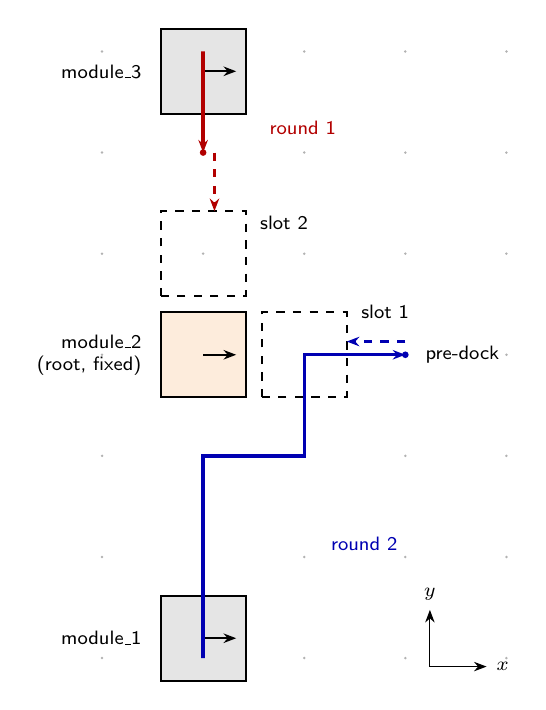
\begin{tikzpicture}[x=12cm, y=12cm, font=\sffamily\scriptsize, >={Stealth[length=1.6mm]}]
  % grid nodes
  \foreach \i in {-1,...,3} \foreach \j in {-3,...,3}
    \fill[black!30] (0.107*\i, 0.107*\j) circle (0.5pt);
  % goal slots
  \draw[thick, dashed] (0.107-0.045,-0.045) rectangle (0.107+0.045,0.045);
  \draw[thick, dashed] (-0.045,0.107-0.045) rectangle (0.045,0.107+0.045);
  \node[anchor=west] at (0.157,0.045) {slot 1};
  \node[anchor=west] at (0.050,0.140) {slot 2};
  % start poses
  \draw[thick, fill=black!10] (-0.045,-0.345) rectangle (0.045,-0.255);
  \draw[thick, fill=stmorange] (-0.045,-0.045) rectangle (0.045,0.045);
  \draw[thick, fill=black!10] (-0.045,0.255) rectangle (0.045,0.345);
  \node[anchor=east] at (-0.055,-0.300) {module\_1};
  \node[anchor=east, align=right] at (-0.055,0) {module\_2\\(root, fixed)};
  \node[anchor=east] at (-0.055,0.300) {module\_3};
  \foreach \y in {-0.3,0,0.3} \draw[->, thick] (0,\y) -- (0.035,\y);
  % round 1: module_3
  \draw[very thick, red!70!black, ->] (0,0.3) -- (0,0.321) -- (0,0.214);
  \draw[thick, red!70!black, dashed, ->] (0.012,0.214) -- (0.012,0.152);
  \fill[red!70!black] (0,0.214) circle (1.2pt);
  \node[anchor=west, text=red!70!black] at (0.06,0.24) {round 1};
  % round 2: module_1
  \draw[very thick, blue!70!black, ->] (0,-0.3) -- (0,-0.321) -- (0,-0.107)
       -- (0.107,-0.107) -- (0.107,0) -- (0.214,0);
  \draw[thick, blue!70!black, dashed, ->] (0.214,0.014) -- (0.152,0.014);
  \fill[blue!70!black] (0.214,0) circle (1.2pt);
  \node[anchor=west, text=blue!70!black] at (0.125,-0.2) {round 2};
  \node[anchor=west] at (0.225,0) {pre-dock};
  % axes
  \draw[->] (0.24,-0.33) -- (0.30,-0.33) node[right] {$x$};
  \draw[->] (0.24,-0.33) -- (0.24,-0.27) node[above] {$y$};
\end{tikzpicture}
\caption{L-shape test: planned grid routes from the spawn poses (grid nodes every \SI{0.107}{m}). Arrows in the squares show the module heading. Solid lines: routes to the pre-dock points (dots); dashed: back-in approach to the slot, drawn slightly offset from the route.}
\label{fig:nav-lshape}
\end{figure}

\textbf{Next steps.}
\begin{itemize}[topsep=2pt,itemsep=2pt,parsep=0pt,beginpenalty=10000]
\item Implement the avoidance between moving modules (prioritised planning, conflict resolution, rescheduling, execution preconditions) and run the two-module conflict scenarios.
\item Check and correct the lateral error $e_y$ during the approach.
\item Skip the first grid node of a route when it lies behind the module. In the L-shape test the nearest node is \SI{2.1}{cm} on the far side for both modules, so each first turns towards it and then turns back.
\item Add the helper-free L/R docking to \texttt{algo\_node} and run the side-by-side test of Table~\ref{tab:nav-n1}.
\item Join docked modules in the simulation with Gazebo detachable joints.
\item Replace the ground-truth poses with AprilTag localisation.
\end{itemize}

\clearpage
% ================================================================
\section{Helper-Free Side (L/R) Docking}
\label{sec:side-docking}

\subsection{Gap in the Original Method}

Our reconfiguration planner follows the parallel self-assembly method of Liu et al.\ \cite{liu2023} (Section~\ref{sec:nav-plan}). In that method, an L/R connection, where a module docks with its wheel face, needs a \textbf{helper module} to lift the moving module during docking. This adds time, adds extra tasks to the assembly sequence, and needs an extra module that is free and close by. For this reason, Section~\ref{sec:nav-dock} proposed that L/R connections might be excluded.

Docking through a wheel face is hard for two reasons:

\begin{enumerate}[topsep=2pt,itemsep=2pt,parsep=0pt,leftmargin=1.5em]
\item \textbf{The wheel face cannot move sideways.} The face points along the wheel axle, and a differential-drive module cannot move along its axle. It cannot simply drive its wheel face straight into the parent, as it does for T/B connections.
\item \textbf{The wheel face turns while the module drives.} The face is part of the wheel, so its angle changes as the module moves. The EP connector only mates when the pattern on the wheel face lines up with the pattern on the parent face, so the final wheel angle is also a docking condition.
\end{enumerate}

\subsection{Trajectory Planning by Wolfe et al.}

To remove the need for a helper, we use the trajectory planning method of Wolfe et al.\ \cite{wolfe2010}. Their modules also dock through their wheels, so, like ours, the final wheel angle must be controlled, not only the position and heading. Their method plans the whole final motion so that the docking wheel arrives at the correct position, with the correct heading, and at the correct wheel angle.

There is one difference. In Wolfe et al.\ the wheel face has two-fold symmetry, so a valid wheel angle repeats every $\pi$. Our EP face has four-fold symmetry, so a valid wheel angle repeats every $\pi/2$. This gives us twice as many valid final wheel angles to choose from.

\subsection{Turn, Straight, Turn, Straight}

Wolfe et al.\ show that the module can always reach the goal with four segments: \textbf{turn, straight, turn, straight}. Each turn is a pivot about the docking wheel: the docking wheel is held still and only the other wheel turns. This keeps the problem simple, because the docking wheel's angle then changes \emph{only} during the two straights. The rotation of the docking wheel is just the sum of the two straight lengths divided by the wheel radius.

Figure~\ref{fig:side-dock-steps} shows an example:

\begin{enumerate}[topsep=2pt,itemsep=2pt,parsep=0pt,leftmargin=1.5em]
\item \textbf{Turn.} At the start pose $\mathbf{p}_0$, the module pivots about its docking wheel to face the intermediate point $\mathbf{p}_1$.
\item \textbf{Straight.} The module drives straight from $\mathbf{p}_0$ to $\mathbf{p}_1$ (Figure~\ref{fig:side-dock-2}).
\item \textbf{Turn.} At $\mathbf{p}_1$, it pivots about the docking wheel again to the final heading $\theta_f$, so its wheel face is in line with the parent face (Figure~\ref{fig:side-dock-3}).
\item \textbf{Straight.} It drives straight from $\mathbf{p}_1$ to $\mathbf{p}_f$, sliding the wheel face along the line of the parent face until it docks (Figure~\ref{fig:side-dock-4}).
\end{enumerate}

\begin{figure}[!htbp]
	\centering
	\begin{subfigure}[b]{0.45\textwidth}
		\centering
		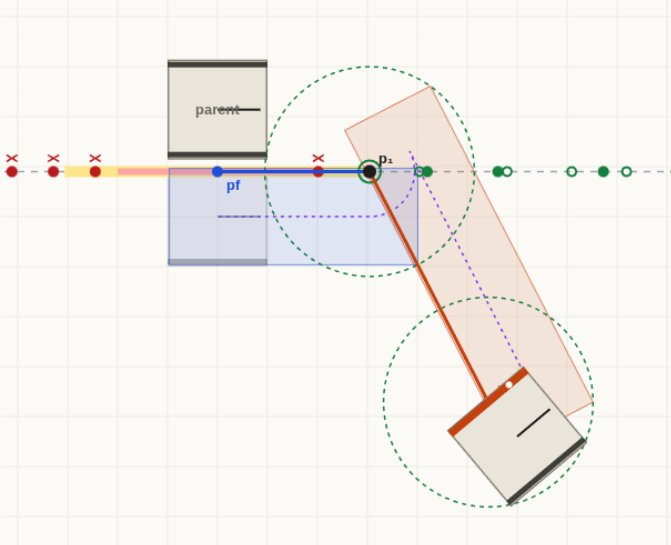
\includegraphics[width=\linewidth]{../image/side_dock_1_start.png}
		\caption{Start pose $\mathbf{p}_0$ and the planned path.}
		\label{fig:side-dock-1}
	\end{subfigure}
	\hfill
	\begin{subfigure}[b]{0.45\textwidth}
		\centering
		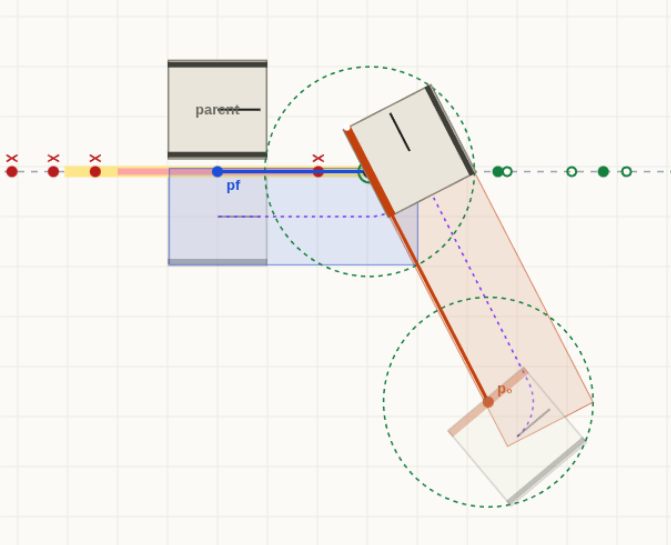
\includegraphics[width=\linewidth]{../image/side_dock_2_first_straight.png}
		\caption{After the first turn and straight, at $\mathbf{p}_1$.}
		\label{fig:side-dock-2}
	\end{subfigure}
	\par\vspace{6pt}
	\begin{subfigure}[b]{0.45\textwidth}
		\centering
		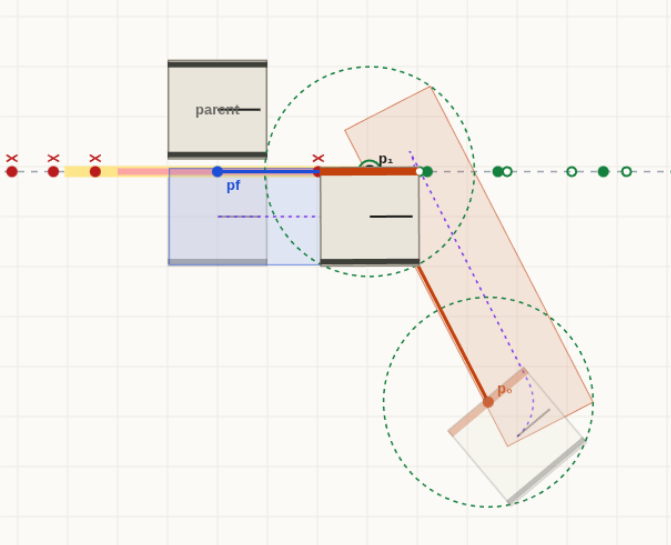
\includegraphics[width=\linewidth]{../image/side_dock_3_second_pivot.png}
		\caption{After the second turn, at heading $\theta_f$.}
		\label{fig:side-dock-3}
	\end{subfigure}
	\hfill
	\begin{subfigure}[b]{0.45\textwidth}
		\centering
		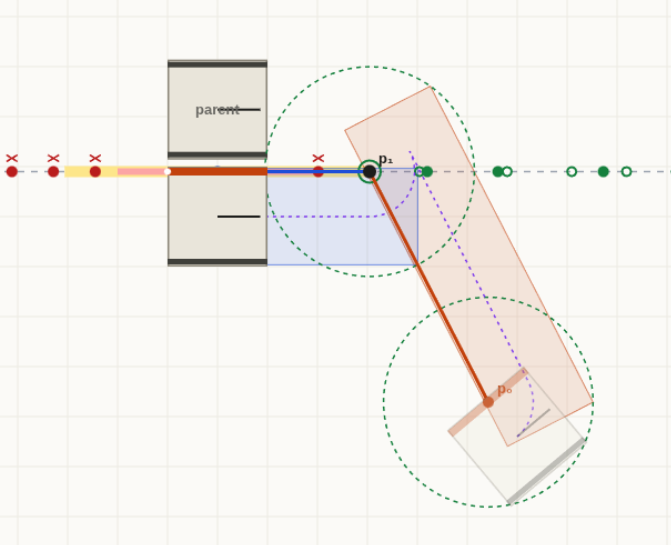
\includegraphics[width=\linewidth]{../image/side_dock_4_docked.png}
		\caption{After the final straight, docked at $\mathbf{p}_f$.}
		\label{fig:side-dock-4}
	\end{subfigure}
	\caption{Example of helper-free L/R docking with turn, straight, turn, straight. The orange line is the path of the docking wheel. The dots on the dashed line are candidate positions for $\mathbf{p}_1$.}
	\label{fig:side-dock-steps}
\end{figure}

\subsection{Wheel Angle Constraint}

Because the docking wheel only turns during the straights, the plan is two lines added together. The only thing left is to choose $\mathbf{p}_1$ so that the total length of the two lines turns the docking wheel to a valid angle.

Let $\phi_{d,0}$ be the starting angle of the docking wheel, $\phi_f$ the target wheel angle and $r$ the wheel radius. With four-fold symmetry, the final wheel angle may be $\phi_f + k\pi/2$ for any integer $k$, so the total distance driven must be
\begin{equation}
|\mathbf{p}_1 - \mathbf{p}_0| + |\mathbf{p}_f - \mathbf{p}_1| = c_k = r\left(\phi_f - \phi_{d,0} + k\frac{\pi}{2}\right), \qquad k \in \mathbb{Z},\ c_k > 0.
\end{equation}
The point $\mathbf{p}_1$ must also lie on the line through $\mathbf{p}_f$ along the final driving direction, so that the last straight runs along the parent face. Each $k$ therefore gives one candidate $\mathbf{p}_1$ on that line. Candidates whose final straight is too short, or that would cross the parent, are rejected (marked $\times$ in Figure~\ref{fig:side-dock-steps}), and the cheapest valid plan is chosen.

\subsection{Simulation Implementation}

The method is implemented in the \texttt{msrr\_control} ROS~2 package and tested in Gazebo. It has two parts: a planner (\texttt{wheel\_dock\_plan.py}, no ROS code) and an executor (\texttt{wheel\_dock.py}). The central controller (\texttt{algo\_node}) first drives the moving module along its grid route to a pre-dock point (Section~\ref{sec:nav-plan}). For an L/R connection, it then hands control to the executor. Both parts read the module pose from Gazebo ground truth and the wheel angles from \texttt{joint\_states}.

\textbf{Planner.} The planner computes one plan from the module's current pose and docking-wheel angle:
\begin{itemize}[topsep=2pt,itemsep=2pt,parsep=0pt]
\item The goal $\mathbf{p}_f$ is the docking-wheel centre at the target slot, moved \SI{3}{mm} away from the parent so that the EP magnets close the last gap.
\item $\mathbf{p}_1 = \mathbf{p}_f + s\,\mathbf{h}(\theta_f)$ is searched over $\SI{0.16}{m} \le |s| \le \SI{0.5}{m}$ on both sides of $\mathbf{p}_f$, with the first straight driven forwards or in reverse. The valid values of $s$ are the roots of $\sin\!\big(2(\phi_{d,\mathrm{end}}(s) - \phi_f)\big)$, which is zero exactly when the final wheel angle is a valid angle modulo $\pi/2$. They are found by sign change and bisection.
\item Each candidate is checked for collisions with the parent: the body swept by each pivot must clear the parent, and the body square is checked against the parent square (separating axis test) every \SI{1}{cm} along both straights.
\item The cost is $\sqrt{2}\,(\text{straight length}) + W\,(|\Delta\theta_1| + |\Delta\theta_2|)$. Candidates with at least \SI{1}{cm} clearance are preferred.
\end{itemize}

\textbf{Executor.} The executor runs the four segments in closed loop at \SI{10}{Hz}:
\begin{itemize}[topsep=2pt,itemsep=2pt,parsep=0pt]
\item \textbf{Pivot:} it commands $v = \pm\omega W/2$, so that the speed of the docking wheel is zero, and stops when the heading error is below \SI{0.03}{rad}.
\item \textbf{Straight:} it drives with a proportional speed command, corrects heading and sideways error, and stops when the docking wheel is within \SI{3}{mm} of the segment end.
\item If a segment ends more than \SI{1}{cm} away from the plan, the rest of the plan is computed again from the current pose.
\item At the end, the wheel-angle error modulo $\pi/2$ is reported, and the dock is accepted if it is below \SI{0.2}{rad}.
\end{itemize}

The model values are $r = \SI{0.05}{m}$, $W = \SI{0.09665}{m}$, body size \SI{0.107}{m} and top wheel speed \SI{0.049}{m/s}.

\subsection{Simulation Results}

\textbf{Test.} Two modules were spawned \SI{0.3}{m} apart along $y$, both facing $+x$, with target connection \texttt{1,L,0,R}. The planner chose \texttt{module\_1} as the root. \texttt{module\_2} must dock its left wheel face onto the root's right face, so it has to finish on the far side of the root. The run was repeated twice from the same start.

Figure~\ref{fig:sim-side-dock-shots} shows Gazebo screenshots of the successful run (top view), and Figure~\ref{fig:sim-side-dock-path} compares the planned and executed paths. Table~\ref{tab:sim-side-dock} lists the measured values.

\begin{figure}[!htbp]
	\centering
	\begin{subfigure}[b]{0.31\textwidth}
		\centering
		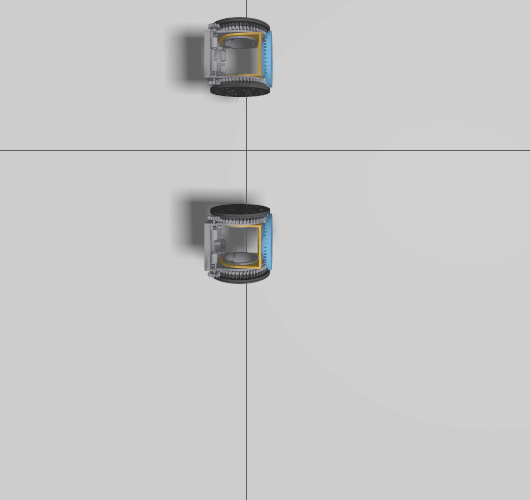
\includegraphics[width=\linewidth]{../image/sim_side_dock_start.png}
		\caption{Start. Root below, moving module above.}
		\label{fig:sim-shot-start}
	\end{subfigure}
	\hfill
	\begin{subfigure}[b]{0.31\textwidth}
		\centering
		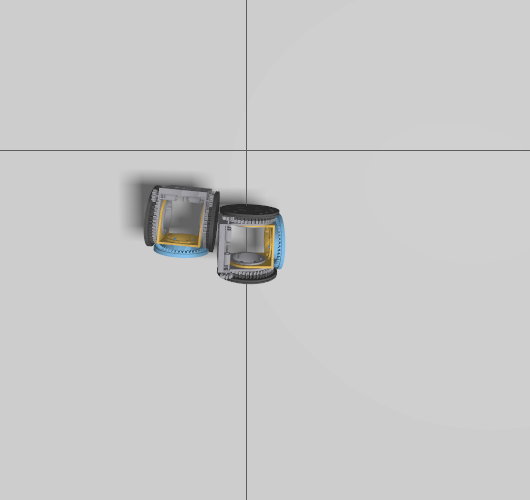
\includegraphics[width=\linewidth]{../image/sim_side_dock_nav_collision.png}
		\caption{Navigation: the module hits the corner of the root.}
		\label{fig:sim-shot-collision}
	\end{subfigure}
	\hfill
	\begin{subfigure}[b]{0.31\textwidth}
		\centering
		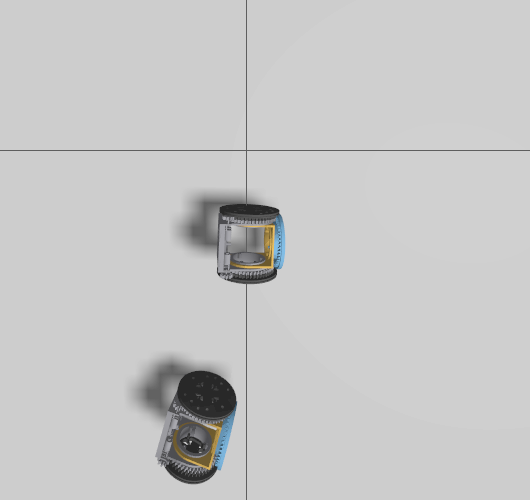
\includegraphics[width=\linewidth]{../image/sim_side_dock_dock_start.png}
		\caption{Pre-dock point reached; the wheel dock starts.}
		\label{fig:sim-shot-dockstart}
	\end{subfigure}
	\par\vspace{6pt}
	\begin{subfigure}[b]{0.31\textwidth}
		\centering
		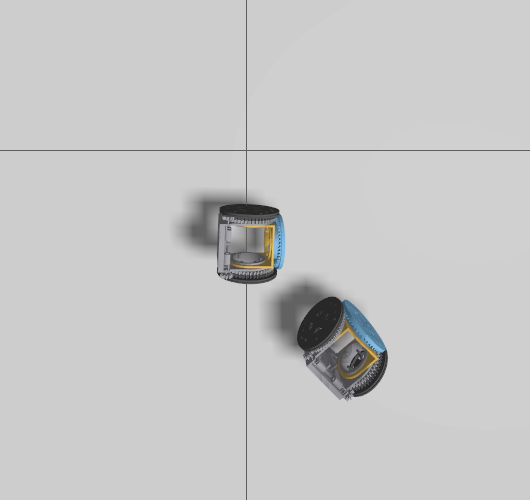
\includegraphics[width=\linewidth]{../image/sim_side_dock_straight1.png}
		\caption{First straight, towards $\mathbf{p}_1$.}
		\label{fig:sim-shot-straight1}
	\end{subfigure}
	\hfill
	\begin{subfigure}[b]{0.31\textwidth}
		\centering
		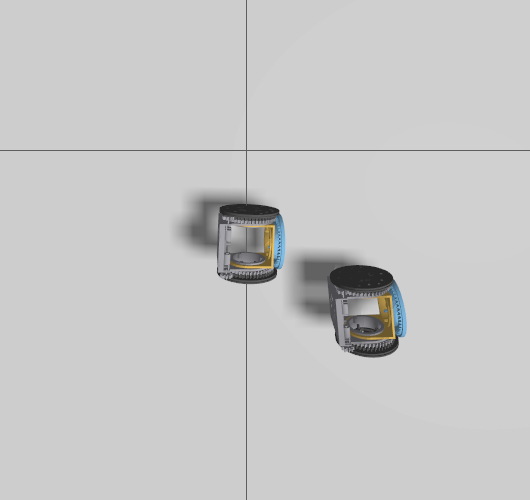
\includegraphics[width=\linewidth]{../image/sim_side_dock_pivot2.png}
		\caption{At $\mathbf{p}_1$ after the second pivot.}
		\label{fig:sim-shot-pivot2}
	\end{subfigure}
	\hfill
	\begin{subfigure}[b]{0.31\textwidth}
		\centering
		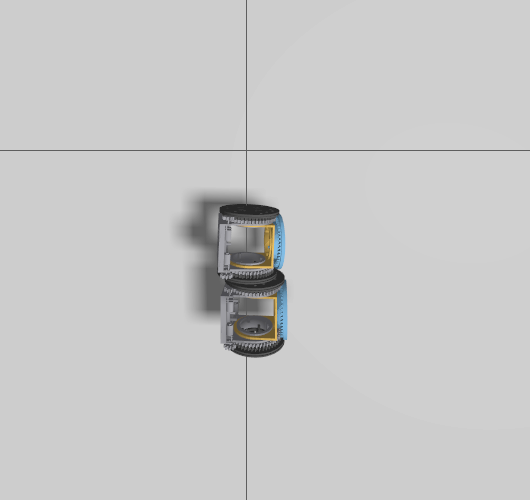
\includegraphics[width=\linewidth]{../image/sim_side_dock_docked.png}
		\caption{Docked after the final straight (in reverse).}
		\label{fig:sim-shot-docked}
	\end{subfigure}
	\caption{Gazebo top view of helper-free L/R docking (connection \texttt{1,L,0,R}).}
	\label{fig:sim-side-dock-shots}
\end{figure}

\begin{figure}[!htbp]
	\centering
	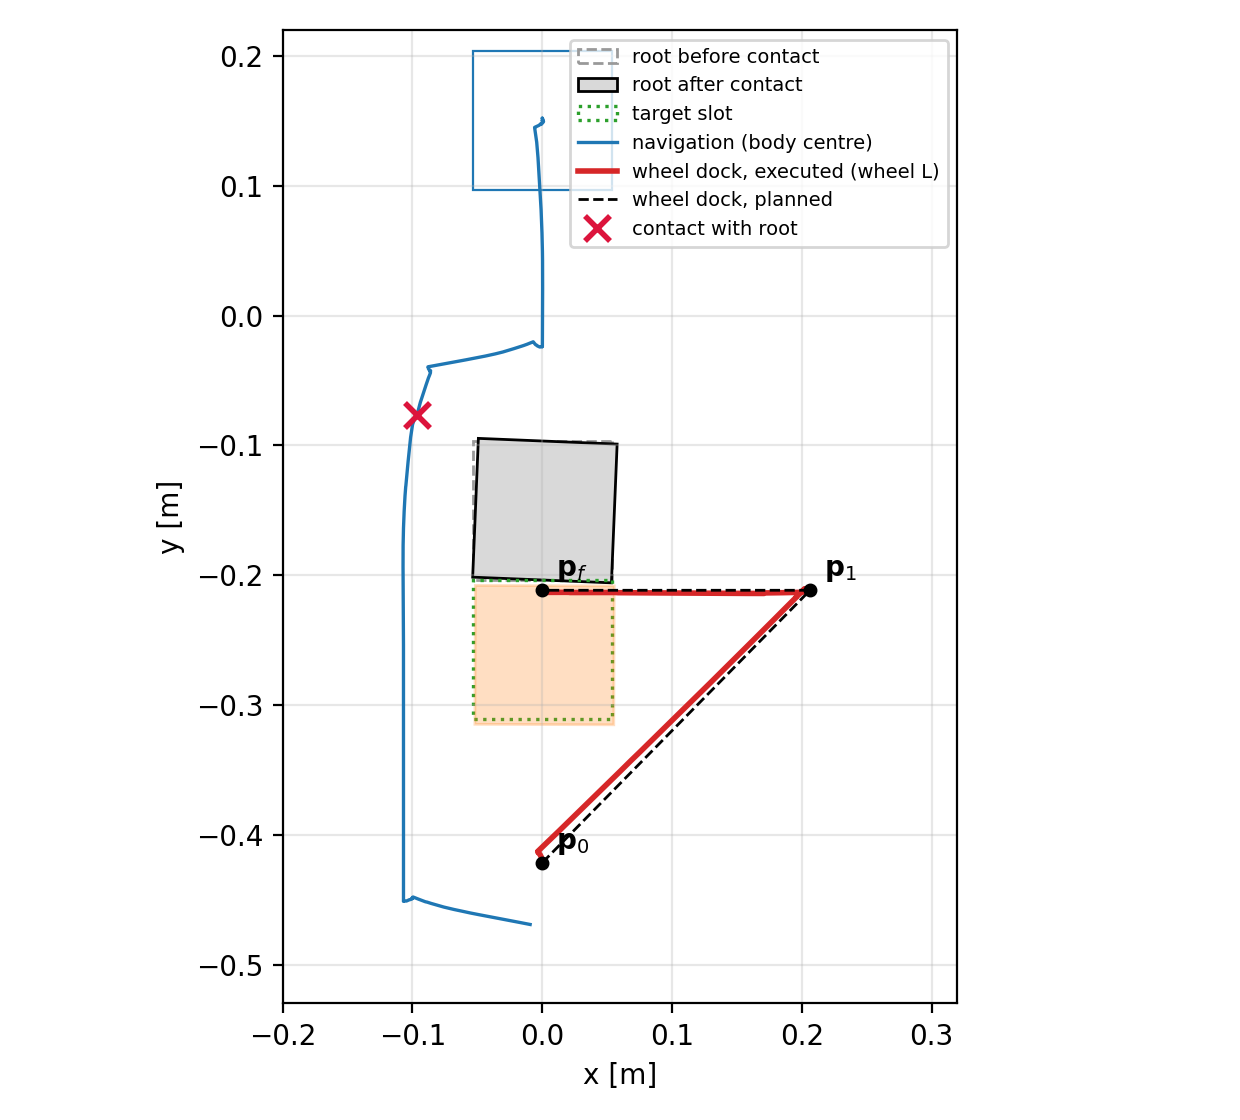
\includegraphics[width=0.62\textwidth]{../image/sim_side_dock_path.png}
	\caption{Planned and executed paths of the successful run. The blue line is the grid navigation to the pre-dock point. The red line is the executed path of the docking wheel and the dashed line is the plan. The root was pushed when the moving module hit it during navigation.}
	\label{fig:sim-side-dock-path}
\end{figure}

\begin{table}[!htbp]
\centering
\caption{Measured values of the successful run (ground truth from Gazebo).}
\label{tab:sim-side-dock}
\small
\begin{tabular}{@{}lll@{}}
\toprule
\textbf{Quantity} & \textbf{Plan} & \textbf{Executed} \\
\midrule
First straight (forward) & \SI{0.294}{m} & \SI{0.289}{m} \\
Second straight (reverse) & \SI{0.206}{m} & \SI{0.199}{m} \\
Movement of the held wheel in pivot 1 / pivot 2 & 0 / 0 & \SI{9.2}{mm} / \SI{3.1}{mm} \\
Final docking-wheel position error (along / normal to face) & -- & \SI{2.1}{mm} / \SI{1.6}{mm} \\
Final heading error (world / relative to parent) & -- & \ang{0.2} / \ang{2.2} \\
Final wheel-angle error (mod $\pi/2$) & 0 & \SI{0.046}{rad} (\ang{2.7}) \\
Effective rolling radius & \SI{0.0500}{m} & \SI{0.0496}{m} \\
Wheel-dock time / whole run (sim time) & -- & \SI{16.2}{s} / \SI{52.5}{s} \\
\bottomrule
\end{tabular}
\end{table}

The four-segment plan works as intended. During both pivots, the docking wheel's joint angle did not change, so the wheel only turned during the two straights. The module finished \SI{2}{mm} from $\mathbf{p}_f$, and the wheel angle was \SI{0.046}{rad} from a valid angle, which is about \SI{2.3}{mm} of rolling. However, the second run from the same start \textbf{failed} with ``no clear docking plan'', so the method is not yet reliable.

\subsection{Flaws Found}

\begin{enumerate}[topsep=2pt,itemsep=2pt,parsep=0pt,leftmargin=1.5em]
\item \textbf{Collision during navigation.} The grid cell (\SI{0.107}{m}) is equal to the body width, so the route around the root leaves no clearance, and the turn-then-drive controller cuts the corner (Figure~\ref{fig:sim-shot-collision}). The moving module hit the root, which moved it by \SI{2}{mm} and rotated it by \ang{2.4} in the first run and by \ang{3.4} in the second run. This happens before the wheel dock, but it breaks the dock.
\item \textbf{The goal does not follow the parent.} The goal $\mathbf{p}_f$ is taken from the fixed target slot in the world, not from the parent's actual pose. In the first run, the module therefore docked with a \ang{2.2} tilt relative to the parent face, and the gap was about \SI{4.3}{mm} at the face centre instead of \SI{3}{mm}. In the second run, the rotated root blocked every candidate path in the collision check, so no plan was found.
\item \textbf{The held wheel slips during pivots.} In Gazebo, the body does not rotate exactly about the held wheel. The docking wheel moved \SI{9.2}{mm} in the first pivot, so the executed straights were 5 to \SI{8}{mm} shorter than planned. The plan is only recomputed if the error exceeds \SI{1}{cm}, so this error is not corrected.
\item \textbf{Straights end on position, not on wheel angle.} A straight stops when the measured position reaches its end, so the final wheel angle depends on the rolling radius. The effective radius in Gazebo is \SI{0.0496}{m}, not \SI{0.05}{m}, and together with the pivot slip this gave the \SI{0.046}{rad} wheel-angle error. The acceptance tolerance (\SI{0.2}{rad}, about \SI{10}{mm} of rolling) is loose. It has not yet been checked against what the EP face pattern needs.
\item \textbf{Heading tolerance at the end of pivots.} A pivot stops within \SI{0.03}{rad} (\ang{1.7}). The remaining heading error is only corrected during the final straight, so the wheel face approaches the parent at a small angle.
\item \textbf{Target wheel angle not calibrated.} The target angle $\phi_f$ is taken from the parent face angle with a mirror offset that is still set to zero, so the absolute alignment of the face patterns has not been verified.
\item \textbf{Ideal sensing and a small test.} The test uses ground-truth pose without noise, only two modules and one start configuration. The three-module side-by-side test (Table~\ref{tab:nav-n1}) has not been run.
\end{enumerate}

\textbf{Next steps.} Add a clearance margin to navigation (a larger grid or an inflated root cell), compute $\mathbf{p}_f$ from the parent's measured pose at the start of the dock, end the straights on the docking-wheel encoder angle, recompute the plan after each pivot, and repeat the test over many start poses to measure the success rate.

\clearpage
% ================================================================
\section{Preparation for Phase B: EP Magnet}
\label{sec:phase-b-magnet}

The docking system uses an Electro-Permanent Magnet (EPM) connector based on SMORES-EP \cite{tosun2016}. Each EP unit pairs an AlNiCo~5 magnet (low coercivity, switchable) with an NdFeB magnet (high coercivity, fixed) between steel pole pieces, wound with a copper coil. 

\begin{figure}[!htbp]
    \centering
    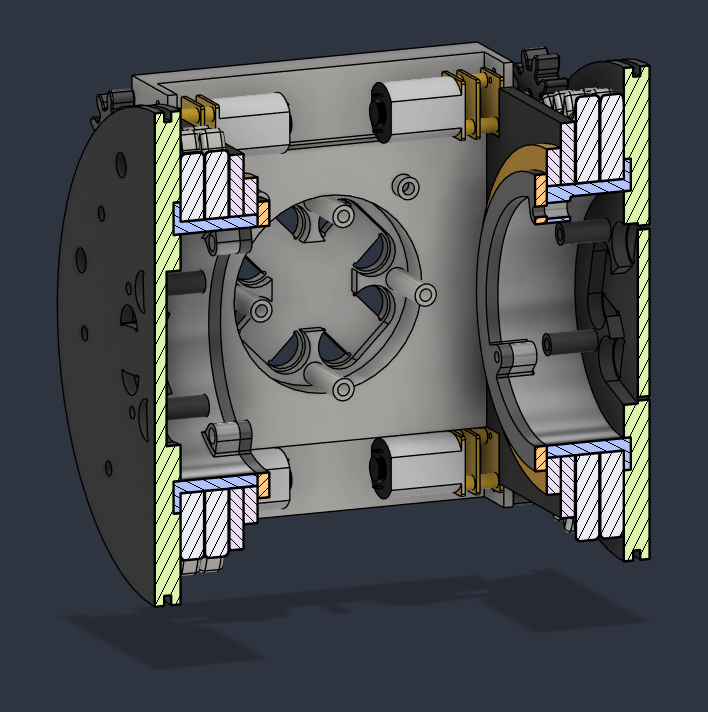
\includegraphics[width=0.6\textwidth]{../image/inside_rectangular_magnet_housing.png}
    \caption{Interior view of the rectangular magnet housing.}
    \label{fig:cad-magnet-housing}
\end{figure}

\textbf{Operating principle:} A current pulse through the coil reverses AlNiCo~5 magnetisation while NdFeB stays fixed. Fields aligned $\rightarrow$ \textbf{ON} (attract); fields opposed $\rightarrow$ \textbf{OFF} (release). No power needed to hold either state.

The original EP-Face connector was developed for a significantly smaller robotic framework. To accommodate our larger target module dimensions of $100\times100\times100$~mm, we had to redesign the baseline architecture. Furthermore, due to the strict standard sizes of magnets available in the Thai market, we altered the core magnet dimensions and completely recalculated the system's electrical and mechanical properties to ensure compatibility and structural integrity.

\subsection{System Architecture and Parametric Scaling}
To fulfill the increased load requirements of our larger module, we scaled several primary parameters from the original reference design:
\begin{itemize}
    \item \textbf{Magnet Dimensions:} The original design utilized $4.76 \times 9.53$~mm magnets. We increased this to $5 \times 15$~mm for both the high-coercivity NdFeB N52 and low-coercivity AlNiCo 5 cylinder magnets.
    \item \textbf{Module Integration:} The original magnets were arranged in a $\varnothing 42$~mm ring. To fit our larger module face, the 4 EP magnets are now arranged within a $\varnothing 50$~mm ring. 
    \item \textbf{Physical Footprint:} The overall length of our EP magnet assembly is $25.6$~mm. The pole piece body has a diameter of $10.6$~mm, while the protruding contact foot has a diameter of $9.6$~mm. The total height of the pole piece is $11.8$~mm, with the contact plane extending $0.5$~mm outward from the module face.
    \item \textbf{Weight:} The increased dimensions raise the weight from $10.6$~g to $19.4$~g per EP magnet.
\end{itemize}

\begin{figure}[H]
    \centering
    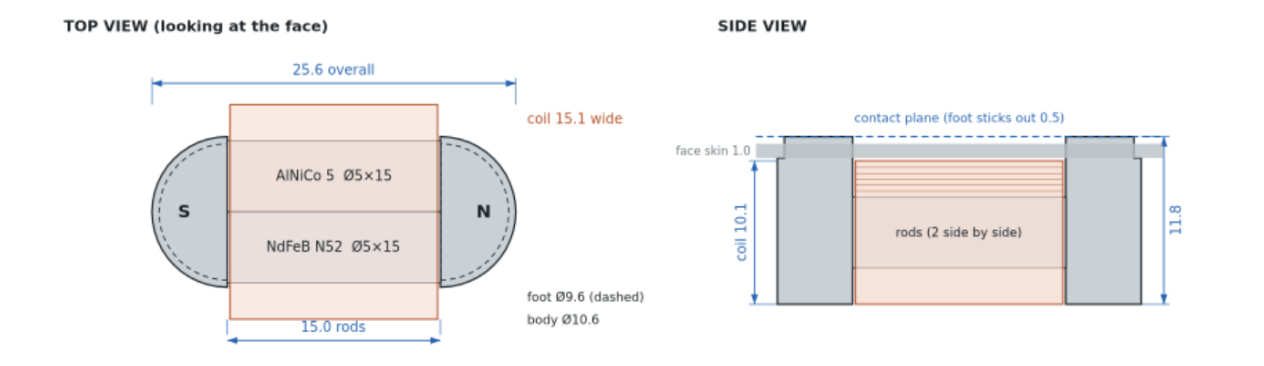
\includegraphics[width=0.9\textwidth]{../image/ep_magnet_diagram.png}
    \caption{Top and side view dimensions of the redesigned $5 \times 15$~mm EP Magnet.}
    \label{fig:ep_diagram}
\end{figure}

\begin{figure}[H]
    \centering
    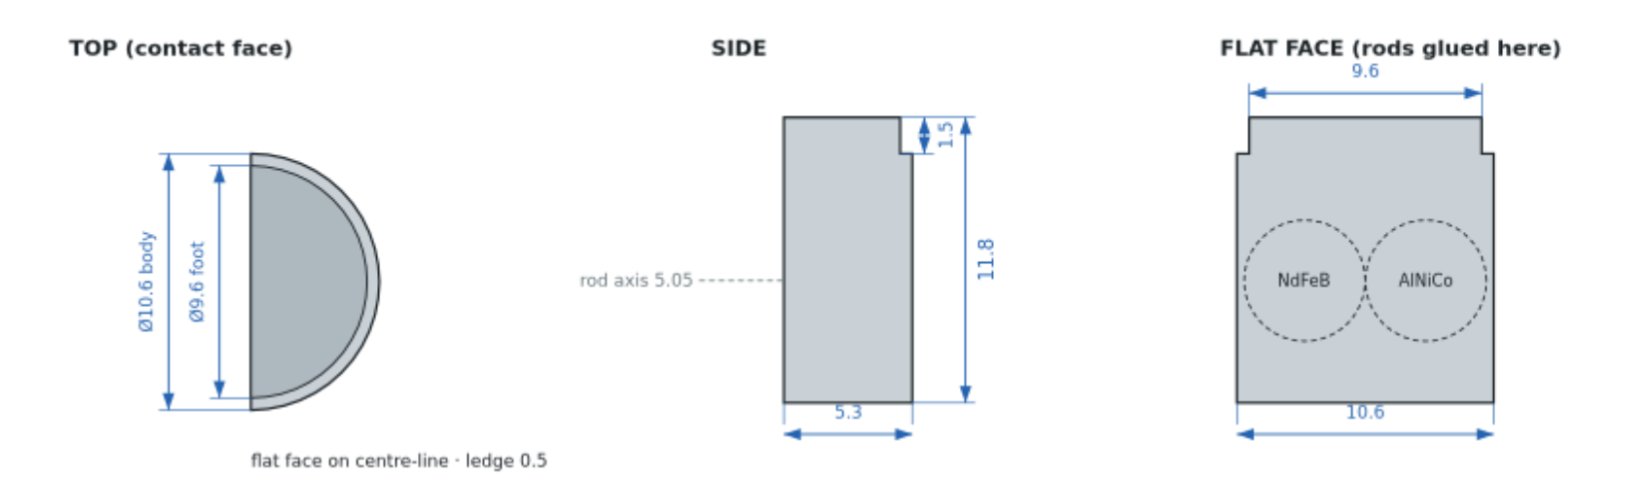
\includegraphics[width=0.9\textwidth]{../image/pole_piece_drawing.png}
    \caption{Detailed mechanical drawing of the low-carbon steel pole piece, illustrating the body and protruding contact foot.}
    \label{fig:pole_piece}
\end{figure}

\subsection{Coil Design and Electrical Specifications}
The coil winding was strictly recalculated to maximize the magnetic field without exceeding the physical constraints of the $11.8$~mm pole pieces. 
\begin{itemize}
    \item \textbf{Wire Selection:} We transitioned from the original AWG 30 wire to SWG 28 double-coated enameled copper wire.
    \item \textbf{Winding Configuration:} The coil consists of exactly 210 turns. This is distributed precisely into 6 complete layers, with each layer containing exactly 35 turns.
    \item \textbf{Wire Length:} Due to the capsule shape of the coil wrapped around the two magnet bars, the perimeter expands with each subsequent layer. The first layer has a perimeter of $27.3$~mm, expanding to $40.4$~mm by the sixth layer. The total length of copper wire required per EP magnet is $7115.3$~mm.
\end{itemize}

\begin{figure}[H]
    \centering
    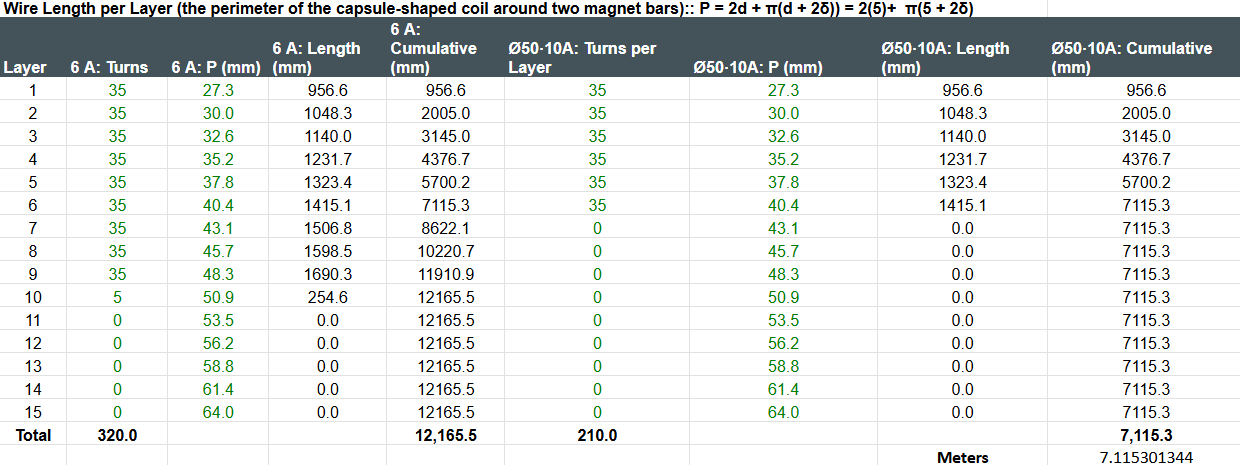
\includegraphics[width=\textwidth]{../image/image_701f62.png}
    \caption{Wire length calculations per layer demonstrating the 6-layer, 210-turn configuration.}
    \label{fig:wire_length}
\end{figure}

\subsubsection{Mathematical Modeling and Formula Derivations}
To ensure the larger system meets the required strength characteristics, the following mathematical formulas were applied to derive our final design parameters:
\begin{itemize}
    \item \textbf{Magnet Area and Total Flux:} The cross-sectional area of the cylindrical magnet rod ($A_{rod}$) is calculated first. $$A_{rod} = \frac{\pi d^2}{4} = \frac{\pi (5)^2}{4} = 19.63 \text{ mm}^2$$ The total magnetic flux ($\Phi$) combines the remnant magnetization of both the NdFeB and AlNiCo magnets. $$\Phi = A_{rod}(Br_{Nd} + Br_{Al}) = 19.63(1.455 + 1.265) = 53.4 \text{ T}\cdot\text{mm}^2$$
    \item \textbf{Minimum Foot Area:} To prevent magnetic saturation within the low-carbon steel, we assume a saturation point ($B_{sat}$) of $1.5$~T to find the minimum required area ($A_{min}$). $$A_{min} = \frac{\Phi}{B_{sat}} = \frac{53.4}{1.5} = 35.6 \text{ mm}^2$$ This minimum area dictates that the minimum foot diameter ($D_{min}$) must be $9.52$~mm. $$D_{min} = \sqrt{\frac{8A_{min}}{\pi}} = 9.52 \text{ mm}$$
    \item \textbf{Magnetic Flux Density in Foot:} By utilizing our selected foot diameter of $9.6$~mm, the actual surface area is $36.2~\text{mm}^2$. This yields an actual magnetic flux density ($B$) at the contact surface. $$B = \frac{\Phi}{A_{foot}} = \frac{53.4}{36.2} = 1.48 \text{ T}$$
    \item \textbf{Holding Force Calibration:} Magnetic holding force is proportional to $B^2 A / (2\mu_0)$. We scale the force directly from the reference paper's maximum baseline force of $90$~N ($F_{paper}$). The scaling multiplier $1.078$ represents the proportional increase in strength due to our larger contact area and stronger flux. The term $f(H)$ acts as a compensation factor for polarization reversal percentage. $$F = F_{paper} \times \frac{(B^2 A)}{(B^2 A)_{paper}} \times f(H) = 90 \text{ N} \times 1.078 \times f(H)$$
    \item \textbf{Mean Length of Turn (MLT):} Because the coil is wrapped around two parallel magnet bars, the winding forms a capsule shape. The length for each coil layer $j$ includes the two straight sides ($2d$) and the two curved ends ($\pi(d + 2\delta_j)$), where $\delta_j$ represents thickness increment per layer. $$MLT_j = 2d + \pi(d + 2\delta_j)$$
    \item \textbf{Coil Resistance:} The total resistance is computed using the resistivity of copper ($\rho$) and the sum of the wire lengths across all layers. $$R = \frac{\rho \sum (N_j \cdot MLT_j)}{A_{wire}} = \frac{1.724 \times 10^{-8} \times 7.12}{0.111 \times 10^{-6}} = 1.105~\Omega$$
    \item \textbf{Current and Magnetic Field (H):} Operating at $12$~V, we estimate an external resistance ($R_{ext}$) of $0.15~\Omega$ for the wiring and MOSFET components. $$I = \frac{V}{(R + R_{ext})} = \frac{12}{1.255} = 9.56 \text{ A}$$ This current generates an applied field capable of fully reversing the AlNiCo 5 polarity. $$H = \frac{NI}{L} = \frac{2008}{0.015} = 134 \text{ kA/m}$$
    \item \textbf{Switching Energy:} The total energy consumed to switch states is calculated by multiplying voltage, current, duration per pulse ($4$~ms), and number of pulses ($3$). $$E = V \cdot I \cdot t \cdot 3 = 12 \times 9.56 \times 0.004 \times 3 = 1.38 \text{ J}$$
\end{itemize}

\subsubsection{Performance Metrics}
The new coil and magnet configuration yields significant performance improvements over the original paper:
\begin{itemize}
    \item \textbf{Electrical Resistance:} Our configuration yields a coil resistance of $1.105~\Omega$, compared to the original $2.08~\Omega$.
    \item \textbf{Magnetic Field and Current:} Driven at $12$~V, the system draws $9.56$~A, generating an operating field of $134$~kA/m. At a peak battery voltage of $12.6$~V, the current reaches $10.04$~A, generating a field of $141$~kA/m. The original design achieved $\approx 6$~A and $121$~kA/m.
    \item \textbf{Holding Force:} The contact surface area is $36.2~\text{mm}^2$ with a magnetic flux density of $\approx 1.48$~T. This results in an expected holding force of $\approx 32$~N per EP pair, yielding a total face holding force of $\approx 97$~N. The original paper averaged $28.3$~N per pair and $88.4$~N per face.
    \item \textbf{Switching Energy:} The required switching energy per face is $\approx 5.5$~J, utilizing three $4$~ms pulses per EP. The original system required $2.5$~J using $3$~ms pulses.
\end{itemize}

\subsection{Current Progress and Procurement Challenges}
\label{sec:ep-progress}
% ======================================================================

The EP magnet follows the design above: an AlNiCo~5 and an NdFeB~N52 rod, both
$\varnothing5\times\SI{15}{mm}$, between two low-carbon steel pole pieces, wound with 210
turns of SWG~28 wire (6 layers $\times$ 35 turns). This period focused on the two
procurement and fabrication problems reported in Progress Report~2: sourcing the AlNiCo~5 magnets and making the pole pieces.

\subsubsection{Procurement}

The AlNiCo~5 magnets, which were the hardest part to source, have now been ordered from a
supplier in China. With this order, all the materials for the first EP magnets have been
purchased or ordered (Table~\ref{pr3:tab:epbom}). The coil driver (half-bridges rated for at
least \SI{10}{A}) has not been bought yet.

\begin{table}[H]
\centering
\caption{EP magnet material status.}
\label{pr3:tab:epbom}
\small
\begin{tabularx}{\linewidth}{l >{\raggedright\arraybackslash}X l}
\toprule
Part & Specification & Status \\
\midrule
AlNiCo 5 rod            & $\varnothing5\times\SI{15}{mm}$ & Ordered from China \\
NdFeB N52 rod           & $\varnothing5\times\SI{15}{mm}$, Ni-Cu-Ni coating & Purchased \\
Magnet wire             & SWG 28, double-coated enamel, \SI{220}{\celsius} class, \SI{98.4}{m} (\SI{0.1}{kg}) & Purchased \\
Pole-piece stock        & SS400 steel rod, $\varnothing\SI{12}{mm}$ & In hand; machine access arranged \\
Kapton tape, CA glue gel& \SI{15}{mm} tape; high-viscosity gel & Purchased \\
Coil driver             & Half-bridge, $\geq\SI{10}{A}$ per channel & Not yet ordered \\
\bottomrule
\end{tabularx}
\end{table}

The wire on hand is enough for the first prototype: at \SI{7.1}{m} per EP magnet
(coil design above), the 8-EP prototype needs about \SI{57}{m} of the \SI{98.4}{m} reel.

\subsubsection{Pole-Piece Fabrication}

External machine shops and wire-cut services would not take the pole pieces because they are
too small. The team will therefore make them in-house from a $\varnothing\SI{12}{mm}$ SS400
steel rod. Use of the milling and cutting machines at the Hans Building has been arranged,
and the team is ready to start milling and cutting the rod to the pole-piece geometry of
Figure~\ref{fig:pole_piece}: a
\SI{10.6}{mm} body, a \SI{9.6}{mm} semicircular contact foot, \SI{11.8}{mm} total height, with
the contact plane standing \SI{0.5}{mm} out from the module face.

SS400 is a general structural steel (JIS G3101). The standard specifies its strength rather
than its carbon content, but the grade is normally a low-carbon steel, so it is expected to
behave like the low-carbon steel assumed in the flux calculation above; this will be confirmed in the first
holding-force test. The \SI{12}{mm} rod leaves about \SI{0.7}{mm} of stock on each side of the
\SI{10.6}{mm} body for machining.

The foot is the dimension that needs the most care. From the flux calculation above, the minimum foot diameter that
keeps the steel below the assumed saturation of \SI{1.5}{T} is \SI{9.52}{mm}, against
the \SI{9.6}{mm} design. A foot machined more than about \SI{0.08}{mm} undersize would
therefore push the steel into saturation and reduce the holding force. The contact faces also
need to be flat and level with each other, since any air gap between two connected faces
reduces the holding force.

\subsubsection{Next Steps}

\begin{enumerate}
  \item Mill and cut the pole pieces from the SS400 rod and measure the foot diameters and heights.
  \item Wind the coils (210 turns, 6 $\times$ 35) and check each coil's resistance against the
        calculated \SI{1.105}{\ohm}.
  \item Assemble the first EP magnets when the AlNiCo~5 rods arrive.
  \item Select and order the $\geq\SI{10}{A}$ half-bridge driver, then run the first
        switching and holding-force tests (EP Face 1st Test in the schedule).
\end{enumerate}

% 

\renewcommand{\refname}{Additional References}
\begin{thebibliography}{9}

\bibitem{tosun2016}
Tosun, T., Davey, J., Liu, C., \& Yim, M. (2016). Design and characterization
of the EP-Face connector. In \textit{IEEE/RSJ International Conference on
Intelligent Robots and Systems (IROS)} (pp.\ 45--51).

\bibitem{liu2023}
Liu, C., Lin, Q., Kim, H., \& Yim, M. (2023). SMORES-EP, a modular robot with
parallel self-assembly. \textit{Autonomous Robots}, 47, 211--228.
doi:10.1007/s10514-022-10078-1.

\bibitem{liu2017}
Liu, C., \& Yim, M. (2019). Configuration recognition with distributed
information for modular robots. In \textit{Robotics Research (ISRR 2017)},
Springer Proceedings in Advanced Robotics, vol.\ 10 (pp.\ 967--983).

\bibitem{mirtich1996}
Mirtich, B. (1996). Fast and accurate computation of polyhedral mass properties.
\textit{Journal of Graphics Tools}, 1(2), 31--50.

\bibitem{wolfe2010}
Wolfe, K.\ C., Kutzer, M.\ D.\ M., Armand, M., \& Chirikjian, G.\ S. (2010).
Trajectory generation and steering optimization for self-assembly of a modular
robotic system. In \textit{IEEE International Conference on Robotics and
Automation (ICRA)}.

\bibitem{binder2019}
Binder, B., Beck, F., K\"onig, F., \& Bader, M. (2019). Multi robot route
planning (MRRP): Extended spatial-temporal prioritized planning. In
\textit{IEEE/RSJ International Conference on Intelligent Robots and Systems
(IROS)} (pp.\ 4133--4139).

\bibitem{binder2017}
Binder, B. (2017). \textit{Spatio-temporal prioritized planning}. Master's
thesis, TU Wien.

\bibitem{kuhn1955}
Kuhn, H.\ W. (1955). The Hungarian method for the assignment problem.
\textit{Naval Research Logistics Quarterly}, 2(1--2), 83--97.

\bibitem{munkres1957}
Munkres, J. (1957). Algorithms for the assignment and transportation problems.
\textit{Journal of the SIAM}, 5(1), 32--38.

\bibitem{microros}
micro-ROS project. \textit{micro-ROS: ROS~2 for microcontrollers}.
\url{https://micro.ros.org}

\end{thebibliography}

\end{document}